%*******10********20********30********40********50********60********70********80
%% ----------------------------------------------------------------
%% Thesis.tex -- MAIN FILE (the one that you compile with LaTeX)
%% ---------------------------------------------------------------- 

%% This template is based on Graduate Thesis written by Sunil Patel,
% (ho based it on the ecsthesis template) under the LaTeX Project Public License.
% which can be found here: http://latex-project.org/lppl/
% in the hope that it will be easier to use and to scale down to your needs
% by Simon Ternsjö in 2013-10



% INSTRUCTIONS:

% The meaning is not to edit this document much, but to fill in information 
% in the different files in the folders;
% Settings, Frontpages, Chapters, Appendices and possibly Files,
% as well as the file Bibliography.bib

% This template is easy to scale down to suite your need, 
% simply comment the input statements explained below


% Set up the document:
\documentclass[a4paper, 12pt, oneside]{Thesis}  % Use the "Thesis" style, based on the ECS Thesis style by Steve Gunn

% Add more package in Package.tex:
% Add your own packages here, 
% these existing packages can be removed if necessary
% not that more packages are imported in Thesis.cls, '
%  but those should not be changed if you don't know what you are doing...

\usepackage[utf8]{inputenc} % for writing other that basic characters
\usepackage{graphicx}
\usepackage{caption}
\usepackage{subcaption}
%\usepackage{biblatex}

%%% Load packages
%\usepackage{amsthm,amsmath}
%\RequirePackage{natbib}
%\RequirePackage[authoryear]{natbib}% uncomment this for author-year bibliography
%\RequirePackage{hyperref}
\usepackage[utf8]{inputenc} %unicode support
%\usepackage[applemac]{inputenc} %applemac support if unicode package fails
%\usepackage[latin1]{inputenc} %UNIX support if unicode package fails

%%Additional packages
%\usepackage[nospace]{cite}
% \usepackage[square, comma, sort&compress]{natbib}
% \usepackage{filecontents}
\usepackage{mathrsfs}
\usepackage{amsmath}
\usepackage{amssymb}
\usepackage{mathtools}
% \usepackage{multicol}
\usepackage{caption}% http://ctan.org/pkg/caption
\captionsetup[table]{format=plain,labelformat=simple,labelsep=period}%
\usepackage{stfloats}
\usepackage[T1]{fontenc}
\usepackage{longtable}
\usepackage{hyperref}
%\usepackage[acronym]{glossaries}
%\usepackage[colorlinks]{hyperref}
\usepackage{booktabs}
\usepackage{csquotes}
\usepackage{dirtytalk}
\usepackage{caption}
%\usepackage{bibunits}

% Include any extra LaTeX packages required
\usepackage[square, numbers, comma, sort&compress]{natbib}  % Use the "Natbib" style for the references in the Bibliography
\usepackage{verbatim}  % Needed for the "comment" environment to make LaTeX comments
\usepackage{booktabs}
\newcommand{\ra}[1]{\renewcommand{\arraystretch}{#1}}
%5%\usepackage{vector}  % Allows "\bvec{}" and "\buvec{}" for "blackboard" style bold vectors in maths
\DeclarePairedDelimiter\set\{\}




% Use if you want:
%5%\graphicspath{Figures/}  % Location of the graphics files (set up for graphics to be in PDF format)
%5%\hypersetup{urlcolor=blue, colorlinks=true}  % Colours hyperlinks in blue, but this can be distracting if there are many links.

% Set your name, the title of the report and more in Administraitve.tex:
% This is where author, university, title and more is defined

% Personal information:
\newcommand{\myAuthorName}  {Gbedegnon Roseric Azondekon}% Author Name
\newcommand{\myAuthorEmail} {roseric@uwm.edu} % Author email
\newcommand{\myTitle}       {\MakeUpperCase{Network Analysis of Scientific Collaboration and Co-authorship of the Trifecta of Malaria, Tuberculosis and HIV/AIDS in Benin.}} % Thesis title goes here
\newcommand{\mySubject}     {Doctor of Philosophy (PhD) in Biomedical and Health Informatics} % Subject goes here
\newcommand{\myKeywords}    {Research collaboration, Co-authorship, Network Analysis, Benin} % Keywords goes hear




% University information
\newcommand{\myUniversity}{The University of Wisconsin - Milwaukee} %The Iniversity name goes here
\newcommand{\myUniversityWeb}{http://www.uwm.edu/} %University Web Site URL Here (include http://
\newcommand{\myDepartment}{Engineering and Applied Sciences} % The Department goes here 
\newcommand{\myDepartmentWeb}{http://uwm.edu/engineering/} % Department Web Site URL Here (include http://)
\newcommand{\myGroup}{Research Group Name}
\newcommand{\myGroupWeb}{Research Group Web Site URL Here (include http://)}
\newcommand{\myFaculty}{College of }
\newcommand{\myFacultyWeb}{Faculty Web Site URL Here (include http://)}

%Degree, program or corse: ex: Master of Science, Engineering Physics
\newcommand{\myDegree}{Doctor of Philosophy\\in Biomedical and Health Informatics\\\\at} % The degree, program or course-name goes here


% can be left untouched, both:
\newcommand{\myDate}{\today}
\newcommand{\myPartyalFulfillment}{A Dissertation submitted in\\ Partial Fulfillment for the Degree of}

%% ----------------------------------------------------------------
\begin{document}
\frontmatter      % Begin Roman style (i, ii, iii, iv...) page numbering


% Here the first pages are imported, you can find them in the Frontpages folder
% Files in the subfolder Fixed does not need to be edited.
% If you don't need any of these sections, simply comment, or delete, the input-row


%% All the pages before the chapters ------------------------------
%Copyright
\clearpage
%\cfoot{\thepage}
\thispagestyle{empty}
\hbox{\ }
\setstretch{2}
%\vfill
\renewcommand{\baselinestretch}{1}
\small\normalsize

\vspace{-.65in}

\begin{center}
\LARGE \MakeUppercase{Network Analysis of Scientific Collaboration and Co-authorship of the Trifecta of Malaria, Tuberculosis and HIV/AIDS in Benin.}\\~\\~\\
\setstretch{1.5}
\large by\\~\\~\\
\LARGE Gbedegnon Roseric Azondekon\\~\\~\\ \large
A Dissertation Submitted in\\
Partial Fulfillment of the\\
Requirements for the Degree of\\~\\
Doctor of Philosophy\\
in Biomedical and Health Informatics\\~\\
at\\~\\
The University of Wisconsin $-$ Milwaukee\\
August 2018
%\large{\copyright \hbox{ }Copyright by Gbedegnon Roseric Azondekon, 2018\\
%All Rights Reserved
%Type your name as it appears in University records
%\\
%}
\end{center}

\vfill


% The Abstract Page
\clearpage
\pagestyle{plain}
\cfoot{\thepage}
%\lhead{}  % Set Left page header to nothing.

%\addtotoc{Abstract}  % Add the "Abstract" page entry to the Contents
\begin{center}
	\textbf{ABSTRACT}\\~\\
	\MakeUppercase{Network Analysis of Scientific Collaboration and Co-authorship of the Trifecta of Malaria, Tuberculosis and HIV/AIDS in Benin.}\\~\\
by\\~\\
Gbedegnon Roseric Azondekon\\~\\
The University of Wisconsin-Milwaukee, 2018\\
Under the Supervision of Professor Susan McRoy
\end{center}
\setstretch{2}
%\abstract{
    %\addtocontents{toc}{\vspace{0em}}  % Add a gap in the Contents, 
                                        %for aesthetics
    %The Thesis Abstract is written here (and usually kept to just this page). 
    %The page is kept centered vertically so can expand into the blank space above the title too \ldots
    Despite the international mobilization and increase in research funding, Malaria, Tuberculosis and HIV/AIDS are three infectious diseases that have claimed more lives in sub Saharan Africa than any other place in the World. Consortia, research network and research centers both in Africa and around the world team up in a multidisciplinary and transdisciplinary approach to boost efforts to curb these diseases. Despite the progress in research, very little is known about the dynamics of research collaboration in the fight of these Infectious Diseases in Africa resulting in a lack of information on the relationship between African research collaborators. This dissertation addresses the problem by documenting, describing and analyzing the scientific collaboration and co-authorship network of Malaria, Tuberculosis and HIV/AIDS in the Republic of Benin.\\
    We collected published scientific records from the Web Of Science over the last 20 years (From January 1996 to December 2016). We parsed the records and constructed the coauthorship networks for each disease. Authors in the networks were represented by vertices and an edge was created between any two authors whenever they coauthor a document together. We conducted a descriptive social network analysis of the networks, then used mathematical models to characterize them. We further modeled the complexity of the structure of each network, the interactions between researchers, and built predictive models for the establishment of future collaboration ties. Furthermore, we implemented the models in a shiny-based application for co-authorship network visualization and scientific collaboration link prediction tool which we named \textbf{AuthorVis}.\\
    %We further applied complex statistical network modeling methods to model the underlying phenomenon influencing collaboration tie establishments.\\
    Our findings suggest that each one of the collaborative research networks of Malaria, HIV/AIDS and TB has a complex structure and the mechanism underlying their formation is not random. All collaboration networks proved vulnerable to structural weaknesses. In the Malaria coauthorship network, we found an overwhelming dominance of regional and international contributors who tend to collaborate among themselves. We also observed a tendency of transnational collaboration to occur via long tenure authors. We also find that TB research in Benin is a low research productivity area. We modeled the structure of each network with an overall performance accuracy of $79.9\%$, $89.9\%$, and $93.7\%$ for respectively the malaria, HIV/AIDS, and TB coauthorship network. \\ 
    Our research is relevant for the funding agencies operating and the national control programs of those three diseases in Benin (the National Malaria Control Program, the National AIDS Control Program and the National Tuberculosis Control Program). %Our tool prototype can help improve grant and research prioritization and resource allocation to funding and help policy makers ensure in the country.
    %Because multidisciplinary and transdisciplinary research approaches have been proven successful in achieving sound and robust findings, we believe that our research is crucial for the future of research funding in Benin and in Africa.
%Other studies have already reported a universal rise in terms of scientific collaborations.  Understanding the structure of these complex networks is capital since it can help improve research prioritization, identification of prolific researchers, better design, strategic planning and implementation of research program, and promote cooperation and translational research initiatives. In this doctoral thesis proposal, we propose to document, describe and analyze the scientific collaboration, and co-authorship of the research conducted in the Republic of Benin on Malaria, Tuberculosis and HIV/AIDS.% Our strategy consists in mining the literature and tracking the scientific papers published in the available scientific database over the last 20 years (From January 1996 to December 2016). Our research is relevant for the funding agencies operating in Benin and the different national control programs of those three diseases in Benin (the National Malaria Control Program, the National AIDS Control Program and the National Tuberculosis Control Program). Our findings will help improve grant and research prioritization and resource allocation to funding and help research organizations as well as national control programs to promote and encourage transdisciplinary and interdisciplinary research in the country. In addition, our results will recommend new approaches and important tools to support the Beninese national control programs via better strategic planning and implementation of public health policies, research and development.  Because multidisciplinary and transdisciplinary research approaches have been proven successful in achieving sound and robust findings, we believe that our research is crucial for the future of research funding in Benin and in Africa. This is why, the last focus of our proposal is the prototyping and evaluation of an online, real-time research collaboration tool to help researchers, governmental agencies and funding organizations promote cooperation and translational research initiative in the republic of Benin.
%}


%\pagebreak
%% The "Funny Quote Page"
\clearpage
\pagestyle{empty}  % No headers or footers for the following pages

%use 1 or vfill to position the quote where it looks good:
\null\vfill\vfill


% Now comes the "Funny Quote", written in italics:

\textit{
    % Write a funny quote here:
    ''We did it, we bashed them, wee Potter’s the one, \\
    and Voldy’s gone moldy, so now let’s have fun!''
}
\begin{flushright}
    % If the quote is taken from someone, their name goes here:
    - Peeves
\end{flushright}


 
\vfill\vfill\vfill\vfill\vfill\null


%%% ----------------------------------------------------------------
% Declaration Page required for the Thesis, your institution may give you a different text to place here
\pagestyle{fancy}  % Finally, implement the FancyHdr headers
\clearpage
\Declaration{

\addtocontents{toc}{\vspace{1em}}  % Add a gap in the Contents, for aesthetics

I, \myAuthorName, declare that this thesis titled, `\myTitle' and the work presented in it are my own. I confirm that:

\begin{itemize} 
\item[\tiny{$\blacksquare$}] This work was done wholly or mainly while in candidature for a research degree at the University of Wisconsin Milwaukee.
 
\item[\tiny{$\blacksquare$}] Where any part of this thesis has previously been submitted for a degree or any other qualification at this University or any other institution, this has been clearly stated.
 
\item[\tiny{$\blacksquare$}] Where I have consulted the published work of others, this is always clearly attributed.
 
\item[\tiny{$\blacksquare$}] Where I have quoted from the work of others, the source is always given. With the exception of such quotations, this thesis is entirely my own work.
 
\item[\tiny{$\blacksquare$}] I have acknowledged all main sources of help.
 
\item[\tiny{$\blacksquare$}] Where the thesis is based on work done by myself jointly with others, I have made clear exactly what was done by others and what I have contributed myself.

\end{itemize}
 
\vspace{10 mm}
 
Signed:\\
\rule[1em]{25em}{0.5pt}  % This prints a line for the signature

Date:\\
\rule[1em]{25em}{0.5pt}  % This prints a line to write the date
}



% The Acknowledgements page, for thanking everyone
\clearpage
\setstretch{1.3} % Reset the line-spacing to 1.3 for body text (if changed)
\acknowledgements{
    \addtocontents{toc}{\vspace{1em}} %Add a gap in the Contents, for aesthetic
    
    % The acknowledgements and the people to thank go here, don't forget to include your project advisor...
    
    % The following are examples of how to word your thanks
    
    First, I would like to express my sincere gratitude to my advisor Prof. Susan McRoy for the continuous support of my Ph.D study, for her patience, motivation, and immense knowledge. Her guidance helped me in all the time of research and writing of this dissertation.
    
    I would also like to offer my special thanks to Dr Charles Welzig and the Welzig Neuroscience and Neurotechnology lab at the Medical College of Wisconsin. I benefited from the computational resource available in the lab to run the analyses and the computational intensive simulations. My thanks also go to Zachary James Harper for his availability. Without his precious support it would not be possible to conduct this research.
    
    My special thanks are extended to Dr Spencer (Chiang Ching) Huang of the Joseph Zilber School of Public Health. He has been crucial to the successful continuation of my PhD journey at the University of Wisconsin Milwaukee. He provided me an opportunity to join, and who gave access to the laboratory and research facilities.
    
    Finally, I would like to thank the rest of my thesis committee: Prof Christine Cheng, and Dr. Rohit Kate, and Dr. Zhang Qing, for their insightful comments, encouragement, and crucial recommendations and suggestions which widen my research from various perspectives.
}


\clearpage
\setstretch{1.3} % Reset the line-spacing to 1.3 for body text (if changed)
%\cfoot{\thepage}
\pagestyle{plain} % The page style headers have been "empty" all this time, 
                  % now use the "fancy" headers as defined before
%\lhead{\emph{Contents}}  % Set the left side page header to "Contents"
\tableofcontents  % Write out the Table of Contents


\pagestyle{plain} % The page style headers have been "empty" all this time, 
                  % now use the "fancy" headers as defined before
%\lhead{\emph{List of Figures}}  % left side page header to "List if Figures"
\setstretch{1.3} % Reset the line-spacing to 1.3 for body text (if changed)
\listoffigures  % Write out the List of Figures


\clearpage  % Start a new page
\setstretch{1.3} % Reset the line-spacing to 1.3 for body text (if changed)
\pagestyle{plain} % The page style headers have been "empty" all this time, 
                  % now use the "fancy" headers as defined before
%\lhead{\emph{List of Tables}}  % left side page header to "List of Tables"
\listoftables  % Write out the List of Tables


\clearpage
\pagestyle{fancy} % The page style headers have been "empty" all this time, 
                  % now use the "fancy" headers as defined before
\setstretch{1.5} % Set the line spacing to 1.5, 
                 % this makes the following tables easier to read
\lhead{\emph{Abbreviations}}  % Set the left side page header to "Abbreviations"
\listofsymbols{ll}  % Include a list of Abbreviations (a table of two columns)
{
  % \textbf{Acronym} & \textbf{W}hat (it) \textbf{S}tands \textbf{F}or \\
   %\textbf{LAH} & \textbf{L}ist \textbf{A}bbreviations \textbf{H}ere \\
   %\textbf{OWL} & \textbf{O}rdinary \textbf{W}izarding \textbf{L}evel\\
   \textbf{AIC} & \textbf{A}kaike's \textbf{I}nformation \textbf{C}riterion \\
   \textbf{AIDS} & \textbf{A}cquired \textbf{I}mmune \textbf{D}eficiency \textbf{S}yndrome \\
   \textbf{AND} & \textbf{A}uthor \textbf{N}ame \textbf{D}isambiguation \\
   \textbf{ARV} & \textbf{A}ntiretroviral \\
   \textbf{AUC} & \textbf{A}rea \textbf{U}nder the \textbf{C}urve \\
   \textbf{AWS} & \textbf{A}mazon \textbf{W}eb \textbf{S}ervices \\
   \textbf{BIC} & \textbf{B}ayesian \textbf{I}nformation \textbf{C}riterion \\
   \textbf{CD4} & \textbf{C}luster of \textbf{D}ifferentiation \textbf{4} \\
   \textbf{CGI} & \textbf{C}ommon \textbf{G}ateway \textbf{I}nterface \\
   \textbf{CI} & \textbf{C}onfidence \textbf{I}nterval \\
   \textbf{CPU} & \textbf{C}entral \textbf{P}rocessing \textbf{U}nit \\
   \textbf{$df$} & \textbf{d}egree of \textbf{f}reedom \\
   \textbf{DOI} & \textbf{D}igital \textbf{O}bject \textbf{I}dentifier \\
   \textbf{ELISA} & \textbf{E}nzyme-\textbf{L}inked \textbf{I}mmunosorbent \textbf{A}ssay \\
   \textbf{ERGM} & \textbf{E}xponential \textbf{R}andom \textbf{G}raph \textbf{M}odel \\
   \textbf{Fig.} & \textbf{F}igure \\
   \textbf{GLM} & \textbf{G}eneralized \textbf{L}inear \textbf{M}odel \\
   \textbf{HIV} & \textbf{H}uman \textbf{I}mmunodeficiency \textbf{V}irus \\
   \textbf{ICL} & \textbf{I}ntegration \textbf{C}lassification \textbf{L}ikelihood \\
   \textbf{JSON} & \textbf{J}ava\textbf{S}cript \textbf{O}bject \textbf{N}otation \\
   \textbf{LNM} & \textbf{L}atent \textbf{N}etwork \textbf{M}odel \\
   \textbf{MeSH} & \textbf{Me}dical \textbf{S}ubject \textbf{H}eadings \\%\\
   \textbf{MCMC} & \textbf{M}arkov \textbf{C}hain \textbf{M}onte \textbf{C}arlo \\
   \textbf{MCMLE} & \textbf{M}onte \textbf{C}arlo \textbf{M}aximum \textbf{L}ikelihood \textbf{E}stimation \\
   \textbf{MDG6} & \textbf{M}illenium \textbf{D}evelopment \textbf{G}oal \textbf{6} \\
   \textbf{MLE} & \textbf{M}aximum \textbf{L}ikelihood \textbf{E}stimation \\
   \textbf{MPLE} & \textbf{M}aximum \textbf{P}seudo\textbf{L}ikelihood \textbf{E}stimation \\
   \textbf{PA} & \textbf{P}referential \textbf{A}ttachment \\
   \textbf{PR} & \textbf{P}recision \textbf{R}ecall \\
   \textbf{REF} & \textbf{R}eference \\
   \textbf{ROC} & \textbf{R}eceiver \textbf{O}perating \textbf{C}haracteristics \\
   \textbf{SAOM} & \textbf{S}tochastic \textbf{A}ctor-\textbf{O}riented \textbf{M}odel \\
   \textbf{SBM} & \textbf{S}tochastic \textbf{B}lock \textbf{M}odel \\
   \textbf{SCI} & \textbf{S}cience \textbf{C}itation \textbf{I}ndex \\
   \textbf{SE} & \textbf{S}tandard \textbf{E}rror \\
   \textbf{SNA} & \textbf{S}ocial \textbf{N}etwork \textbf{A}nalysis \\
   \textbf{SW} & \textbf{S}mall \textbf{W}orld \\
   \textbf{TB} & \textbf{T}uberculosis \\
   \textbf{TERGM} & \textbf{T}emporal \textbf{E}xponential \textbf{R}andom \textbf{G}raph \textbf{M}odel \\
   \textbf{US} & \textbf{U}nited \textbf{S}tates \\
   \textbf{WHO} & \textbf{W}orld \textbf{H}ealth \textbf{O}rganization \\
   \textbf{WOS} & \textbf{W}orld \textbf{O}f \textbf{S}cience \\
}


%\clearpage
\pagestyle{fancy} % The page style headers have been "empty" all this time, 
                  % now use the "fancy" headers as defined before
\lhead{\emph{Physical Constants}}  %L page header to "Physical Constants"
\setstretch{1.5} % Set the line spacing to 1.5, 
                 % this makes the following tables easier to read
\listofconstants{lrcl}  % Include a list of Physical Constants 
                        % (a four column table)
{
% Constant Name & Symbol & = & Constant Value (with units) \\
Speed of Light & $c$ & $=$ & $2.997\ 924\ 58\times10^{8}\ \mbox{ms}^{-\mbox{s}}$ (exact)\\

}



%\clearpage
\pagestyle{fancy} % The page style headers have been "empty" all this time, 
                  % now use the "fancy" headers as defined before
\lhead{\emph{Symbols}}  %Left page header to "Symbols"
\setstretch{1.5} % Set the line spacing to 1.5, 
                 % this makes the following tables easier to read
\listofnomenclature{lll}  % Include a list of Symbols (a three column table)
{
% symbol & name & unit \\
$a$ & distance & m \\
$P$ & power & W (Js$^{-1}$) \\
& & \\ % Gap to separate the Roman symbols from the Greek
$\omega$ & angular frequency & rads$^{-1}$ \\
}


\clearpage
\lhead{}  % Set Left page header to nothing.
\setstretch{1.3}  % Return the line spacing back to 1.3
\pagestyle{empty}  % Page style needs to be empty for this page


%\dedicatory{For/Dedicated to/To my\ldots}
\dedicatory{For my family\ldots}


\addtocontents{toc}{\vspace{2em}}  % Add a gap in the Contents, for aesthetics



\pagebreak
%% The Body -------------------------------------------------------
\setstretch{2}  % Return the line spacing back to 1.3
\mainmatter	  % Begin normal, numeric (1,2,3...) page numbering
\fancyhf{}
\cfoot{\thepage}
\pagestyle{fancy}  % Return the page headers back to the "fancy" style


% Include the chapters of the thesis, as separate files
% Just uncomment the lines as you write the chapters

%*******10********20********30********40********50********60********70********80

% For all chapters, use the newdefined chap{} instead of chapter{}
% This will make the text at the top-left of the page be the same as the chapter
\clearpage  % Start a new page
\lhead{\emph{General Introduction}}  % left side page header to "List of Tables"
\chapter*{\centering General Introduction}
%\chap{General Introduction}
\addcontentsline{toc}{chapter}{General Introduction}
Infectious diseases have long claimed the lives of millions of people worldwide. They disproportionately affect the developing nations where 90\% of the deaths are caused by very few diseases among which Malaria, Tuberculosis (TB) and HIV/AIDS \cite{davis_emerging_2001}. Malaria, TB and HIV/AIDS remain the three major public health concerns in Sub Saharan Africa where they are responsible for high mortality, morbidity rates and impact negatively on the socioeconomic way of life of the populations \cite{gallup_economic_2001,vitoria_global_2009}. These three diseases have been given special attention at the Millenium Declaration in its $6^{th}$ Goal of Millenium Development \cite{assembly_united_2000}. Initiatives such as the US President’s Malaria Initiative, the Global Fund for Malaria, TB and HIV/AIDS and the President’s Emergency Plan for AIDS have led to the investment of more than 70 million of US dollars to encourage Research and Development, Private-Public partnership as well as to reinforce the activities of non-governmental organizations within the healthcare systems of the affected countries \cite{arthur_institute_2014,murray_global_2014,stoops_presidents_2008}.\\
The Global Fund disbursement in 2010 peaked at over 1.45 billion dollars for HIV/AIDS, 416 million dollars for TB and 714 million dollars for Malaria \cite{global_fund_making_2011,world_health_organization_world_2012}. With these financial supports at hand, efforts have led to a sharp increase of public health interventions and many positive public health outcomes in terms of the reduction of mortality and morbidity related to those diseases \cite{barat_four_2006}. For example, in Benin, such increase in public health interventions translated in the financing, successful implementation and sustainability of the entomological surveillance of malaria for more than six years since 2008 \cite{akogbeto_six_2015}.  Encouraged and motivated by the success stories in controlling these diseases, some authors formulated the ambitious zero incidence goal of TB and HIV and the zero death goal of the three diseases by 2015 \cite{joint_united_nations_programme_on_hiv/aids_getting_2010}. \\
After the declaration of the Millenium Challenge Goal 6 in 2000, significant progress has been made in the treatment and prevention of Malaria, TB and HIV/AIDS, leading to the reverse of the mortality and morbidity due to these three diseases. Nevertheless, sub Saharan Africa still carries the burden of these diseases. For example, in 2009, 2.6 million new cases and 1.8 million of death related to HIV were estimated out of which 68\% and 72\% of respectively new cases and deaths were in Africa \cite{joint_united_nations_programme_on_hiv/aids_global_2010}. TB cases were estimated at 9.4 million and 1.3 million deaths out of which HIV-positive cases make up 12\% of all cases and 23\% of all TB deaths \cite{world_health_organization_global_2010}. Although the rapid expansion of vector control strategies worldwide, malaria was responsible of 225 million cases and 781,000 death in 2009 out of which over 90\% were in Africa \cite{world_health_organization_world_2012}. \\
In the Republic of Benin, between 2000 and 2013, the impact of the increase in funding has led to an annual decrease in the incidence of 7.6\%, 0.6\% and 5.2\% respectively in HIV/AIDS, TB and Malaria. Similar results were obtained in terms of prevalence with a decrease of 1.3\% in HIV/AIDS and 0.8\% in TB. Annual death rates decreased also at about 3.1\%, 1.2\% and 5.3\% respectively in HIV/AIDS, TB and Malaria \cite{world_health_organization_world_2012,joint_united_nations_programme_on_hiv/aids_global_2010,world_health_organization_global_2010}.\\
Successful scientific collaborations have led to the eradication of chickenpox and the near eradication of poliomyelitis through the development of vaccines \cite{jamison_disease_2006}. For Malaria and HIV/AIDS, the development of a vaccine has proven significantly difficult to develop despite the decades of active research that has not been successful so far \cite{long_malaria_2016,titti_problems_2007,walker_toward_2008}. This is why researchers need to form continuous and sustainable collaborations through intensive network practices that go beyond the regional boundaries \cite{newman_structure_2001}. Scientific collaborations give researchers the opportunity to work and learn from each other. Such collaborations are further needed to overcome the overgrowing challenge of co-infections of HIV/AIDS and Tuberculosis \cite{corbett_growing_2003,gandhi_hiv_2010}. In the republic of Benin, Malaria, TB and HIV/AIDS have become a common aspect of the public health system. The three are the main impediments of economic and social progress that are characteristics of poverty. According to a 2000 World Health Organization (WHO) press report, malaria slows economic growth on the African continent by 1.3\% each year \cite{world_health_organization_economic_2000}. And it is known that Tuberculosis and HIV/AIDS patients experienced severe economic burden in terms of access to health care, treatment and diagnosis \cite{richter_economic_2014}. The situation is further compounded by the poorly developed immunity among the children and the elderlies, and the predominant malnutrition problem experienced by a majority of the population \cite{jamison_disease_2006}. The disappointing aspect is that the extensive research conducted has not prevented these three diseases from outpacing the proposed solutions and the progress made \cite{akukwe_dont_2006}.\\
Therefore, in this thesis to document, we document, describe and analyze the different aspects of scientific research collaboration of the three leading infectious diseases in the Republic of Benin. The social network analysis of research collaboration approach is chosen to reveal undiscovered knowledge on effort of researchers in working together towards the reduction of the burden of Malaria, TB and HIV/AIDS. Modern times have rendered research and scientific collaborations irreplaceable policy formulations processes. This is because research collaboration forms a stable basis for the provision of evidence based information in the formulation of fundamental principles and guidelines for the elaboration of public health strategies, particularly in developing countries like Benin. For this reason, this thesis focuses on the Network analysis of the scientific collaborations through co-authorship network analysis.
 % Introduction

%*******10********20********30********40********50********60********70********80

% For all chapters, use the newdefined chap{} instead of chapter{}
% This will make the text at the top-left of the page be the same as the chapter

%\chap{Literature Review}
\chap{A review of the related literature on disease research and applications of network analysis}

\section{Brief Overview of Malaria, Tuberculosis and HIV/AIDS}
AIDS is a health condition caused by the Human Immunodeficiency Virus (HIV) \cite{mbulaiteye_hiv_2011,dalessandro_comparison_1995}. HIV infects and attacks the cells that are responsible for the immune system in the body (CD4 cells) that provide protection against infections and illness. The virus infects the human host by making him vulnerable and unable to fight future infections \cite{joint_united_nations_programme_on_hiv/aids_aids_2007}. The virus eventually weakens and kills the CD4 cells resulting in a weak immune system and vulnerability to diseases. HIV is transmitted through body fluids exchange, and the infection exists in four stages. The first stage is the primary infection stage and lasts within 2 to 4 weeks. It is characterized by flu-like symptoms, and the infected person is highly contagious. The second stage is the asymptomatic stage that may last for about ten years, and the infected person does not display significant symptoms of the infections. The third stage is the symptomatic stage. At this stage, the virus weakens the immune system, and the infected person suffers from both mild and chronic symptoms as the infected person suffers opportunistic diseases. Illnesses like malaria and TB in HIV infected subjects, are experienced in a severe manner. The fourth stage is AIDS; it causes death within two years if left untreated \cite{joint_united_nations_programme_on_hiv/aids_aids_2007,whiteside_hiv/aids:_2008}.\\
According to the World Health Organization (WHO) the signs for HIV/AIDS change through the stages of infections as the disease progresses. To determine whether a person is infected, an HIV test needs to be conducted. ELISA method based HIV testing is one of the most common antibody-based testing method characterized by 99\% accuracy rate \cite{mbulaiteye_hiv_2011}. It is recommended that a HIV negative test result should be confirmed after three months because the immune system can sometimes take up to 12 weeks to develop the tested antibodies \cite{centers_for_disease_control_and_prevention_revised_2007}. It is however possible to get false negative results during the 12 weeks window period. The antiretroviral (ARV) drug therapy is initiated when the infected person reaches the third or fourth stage of infection to suppress the virus and boost the immune system. Such measures are taken because there is currently, no cure for HIV and the early initiation of the therapy may result in drug resistance \cite{brenner_we_2016,calmy_hiv_2004,clavel_hiv_2004}.\\
Unlike HIV/AIDS, TB is a highly infectious disease that is caused by a bacteria called \textit{Mycobacterium tuberculosis}. The disease exists in active and inactive forms. The active form, also known as the open disease causes the infected person to suffer and to be highly infectious. The inactive/latent TB infection is not infectious, and the infected individual does not suffer from the signs and symptoms associated with the active disease. Healthy individuals with latent infection have approximately 10\% probability of getting active TB disease over their life. Chances of infection are high in the first two years after the exposure to the bacteria, and in the case where the host develops any form of lung or immune system damage \cite{kaufmann_handbook_2008,zumla_handbook_2009}. On the other hand, in HIV infected individuals co-infected with TB, there exists a 10\% annual chance of developing active TB \cite{raviglione_tuberculosis_1997,sharma_hiv-tb_2005,toossi_impact_2001}. Active TB in adults may result from re-infection with a new strain of TB or perhaps a reaction to the latent infection. Consequently, researchers surmise that silica inhalation, HIV infection, and silicosis are responsible for the high risk of TB infection in the working adults’ population \cite{sharma_hiv-tb_2005,danibrosio_epidemiology_2014}.
TB symptoms are characterized by a chronic cough, night-time fevers, profuse sweating, and significant weight loss within a short time. However, studies show that people with TB can be infectious prior to showing the symptoms or complaining of any form of pulmonary discomfort. In the worst case scenario, TB goes beyond the pulmonary and infects other parts of the body, especially for people infected with HIV. HIV complicates the manifestation of TB in terms of its symptoms and signs in 70\% of the HIV/AIDS infected population suffering from TB \cite{sharma_hiv-tb_2005}. Studies indicate that people with undetected open TB disease are the leading cause of TB infections. Even though TB is a treatable disease, the treatment procedure is extremely aggressive. The treatment procedure for first-time patients entails administration of a six-months dose under close medical supervision termed as directly observed therapy. The other challenge in the treatment is that there are approximately 25\% TB-drugs resistance cases worldwide every year \cite{centers_for_disease_control_and_prevention_cdc_emergence_2006,world_health_organization_multidrug_2010}. Approximately 80\% of people with TB can be cured of their active TB infection, however, HIV and Silicosis increases the risk of reinfection by 20\%. The infection among individuals with silicosis, may cumulatively contribute to lung damage and work inability. Additionally, the HIV/AIDS increases the risk of opportunistic infections, which may result in a poor outcome for the TB treatment \cite{cowie_epidemiology_1994,mulenga_silicosis_2013,rees_silica_2007}.\\
Completing the trifecta is malaria, a parasitic infectious disease caused by the Plasmodium parasites. Even though, malaria is predominantly found in the tropical regions, 48\% of the instances of infections have been experienced in the Northern and Southern parts of America, Asia, and Africa, putting approximately 50\% of the world’s population at risk. The malaria pathogens are \textit{Plasmodium ovale}, \textit{Plasmodium malariae}, \textit{Plasmodium vivax}, and \textit{Plasmodium falciparum} which is the deadliest. The distribution of the disease matches that of its vectors, the female mosquitoes of the genus Anopheles \cite{sinka_global_2012,snow_global_2005}. In the sub-Saharan African countries, the vector of the disease is \textit{Anopheles gambiae s.l}. Malaria has a range of symptoms and signs that manifest differently from one person to another. The most common symptoms are fevers, gastrointestinal symptoms, and fatigue, headaches, and muscle aches. The malaria pathogen infects two hosts, the Anopheles mosquito, and the infected human. When the infected mosquito feeds from an individual, it injects sporozoites into the circulatory system of the bitten person. The sporozoites reside in the liver cells until they become mature schizonts. The schizonts rupture upon maturity and release merozoites, which infect the red blood cells \cite{james_new_1937}. The two most used malaria test are rapid tests using an instant result kit akin to the home pregnancy test device, and the blood smear test that is examined under the microscope for the presence of red blood cells that are infected by the parasite. Treatment entails administration of drugs that range in types. While some malaria drug prescriptions may have a three days dosage, others may have up to one week dosage \cite{alonso_malaria_1993,battle_treatment-seeking_2016}.\\
HIV/AIDS, TB, and Malaria form together a trifecta of diseases caused respectively by a virus, a bacteria, and a parasite.

\section{Network Analysis of Scientific Research collaboration}
Collaboration in science is essential to research and development, knowledge discovery, technology and innovation. 
%It occupies a predominant place in scientometrics. 
The effectiveness of collaboration in science can be measured using scientometrics. According to Leydesdorff and Milojevic \cite{leydesdorff_scientometrics_2012}, scientometrics uses quantitative and computational methods to analyzing and measuring science, communication in science and science policy. %According to the same authors, 
The field of scientometrics emerged from Eugene Garfield’s idea to improve Information Retrieval \cite{eugene_citation_1979}, followed by the creation of the Science Citation Index (SCI) in the 1960s, and the availability of scientific databases references publications. The discipline of Scientometrics is aimed at providing guidance to several research issues involving the measurement of science impact, the measurement of impact journals and institutional units, theories of citation, and the mapping of science. Here, we focus on the mapping of science since it is essential to understanding the dynamic of science, informing policy decisions, and identifying important fields, research groups, as well as specialties based on evidence from the literature \cite{leydesdorff_scientometrics_2012}. Such goals can be achieved by mapping publications, authors and analyzing patterns of collaborations between them.\\
Since the publication of the first co-authored paper in 1665, scientific co-authorship has spread significantly throughout the scientific realm and the number of co-authored scientific publications have tremendously increased \cite{luukkonen_understanding_1992}. According to Wagner \cite{wagner_six_2005}, the increase in international scientific co-authorship has been of a fast growth. International co-authorship originates from international collaborations between scientists. In general, international collaborations have more visibility than national collaborations and often result in publications in high impact journals \cite{glanzel_analysing_2004}.\\
The paradigm of co-authorship network is rooted in network theory. In a co-authorship network, the reasearchers are represented by the set of vertices and the relationship between them are represented by the set of edges. An edge between two researchers in such a network means that they both coauthor a publication. Unlike citation networks, the scientific community has dedicated less attention to co-authorship networks because of the long tradition of citation network analysis in bibliometric \cite{newman_structure_2001,newman_coauthorship_2004}. Nevertheless, the analyses of how complex co-authorship networks form and evolve in time is crucial for identifying leading researchers in a particular scientific domain, describing their extant to collaborate with their peers, and evaluating the impact of their research \cite{gonzalez-alcaide_scientific_2012}. An example of such an investigation is illustrated in Newman scientific collaboration paper series on Biomedical research, physics and computer science co-authorship networks \cite{newman_structure_2001,newman_coauthorship_2004,newman_scientific_2001,newman_scientific_2001-1}.\\
Taking publications as units, the analyses of scientific collaboration facilitate the study of trans and inter-disciplinary research by focusing on the dynamics of the collaboration networks \cite{borner_visualizing_2003}.  In addition, these networks can provide important information regarding cooperation patterns among authors and their status and location in the structures of the scientific community \cite{scharnhorst_models_2012}. Furthermore, Mali et al. \cite{mali_dynamic_2012} assert that co-authorship social network studies are highly relevant for funding organizations for promising and emerging topics support in science.\\
Although many authors have proposed different features for classifying co-authorship networks \cite{andrade_dimensions_2009,rogers_obstacles_2001,sonnenwald_scientific_2007}, the categorization features of Andrade et al. \cite{andrade_dimensions_2009} identifies three levels of classification of scientific collaboration: the cross-disciplinary level with the intradisciplinarity and interdisciplinarity subdimensions, the cross-sectoral level with the intramural and extramural research collaboration subdimensions and the cross-national level including the national and international scientific collaboration subdimensions. For a full description of each level of scientific collaboration, we refer the reader to Mali et al. \cite{mali_dynamic_2012}. \\%Our work focuses more on the intradisciplinarity and interdisciplinarity subdimensions of the cross-disciplinary level.\\
The methods of co-authorship network studies have emerged from social network analysis and graph theory. Such studies heavily relied upon access to scientific collaboration data sources such as SCOPUS, the Web Of Science, PubMed, Medline or even Google Scholar. In general, Mali et al. \cite{mali_dynamic_2012} identify three methodological approaches to studying scientific co-authorship networks:%\\
\begin{displayquote}
(i) basic analysis of network properties using temporal data (usually in the form of a time-series of snapshots), (ii) deterministic approaches to the analysis of scientific co-authorship networks, and (iii) statistical modeling of network dynamics
\end{displayquote}
%Despite the identification of the three methodological approaches, an important body of the literature involving co-authorship network studies rely on the basic analysis of network properties such as 
In addition to the three approaches outlined by Mali et al. \cite{mali_dynamic_2012} and mentioned above, co-authorship networks can be analyzed on the basis of formal network properties, including network degree, density, path, path length, shortest path and the global clustering coefficient. Many scientific collaboration network studies have adopted this graph-based approach to scientific co-authorship investigation. In the next paragraphs, we present and discuss the purpose, methods and the results of some of those studies.\\
Newman \cite{newman_structure_2001} investigated scientific network collaboration in biomedical research, physics and computer science. In this study, Newman collected data from four databases and presented distribution of collaboration networks, demonstrated the presence of clustering and highlights differences between the scientific fields under investigation. According to his findings, Newman \cite{newman_structure_2001} concluded on the "smallworldness" of such networks in which scientists are only separated by shorter paths. In a second paper published the same year, Newman \cite{newman_scientific_2001} provided a deeper analysis of the networks using the same data. He presented a variety of statistical properties of the networks, identified giant collaborative components and study centrality and connectedness measures. In Newman \cite{newman_scientific_2001-1}, the author evaluated various nonlocal network properties including shortest paths and distance between researchers. He proposed a modified version of the standard breadth-first search algorithm for evaluating the geodesic distance between the scientists in the network. He later weighted the networks by the number of paper published by pairs of researchers as well as their number of coauthors, and calculated all the distances using Dijkstra's algorithm. His analyses provided insights in the strength of collaboration in each network. In a last paper in the same series, the author summarized the results of the three previous studies and showed how patterns of collaboration varied between scientists within a scientific field over time \cite{newman_coauthorship_2004}. \\
In another study, Hou et al. \cite{hou_structure_2008} applied a variety of graph-based algorithms to quantify the importance and impact of science, analyzing data retrieved from the Science Citation Index (SCI) over a period expanding from 1978 to 2014. In addition to methods of Social Network Analysis (SNA), the authors used co-occurrence analysis, cluster analysis and frequency analysis of words to describe the microstructure of the scientometrics network, revealing the major collaborative clusters and identifying the center of the scientometrics collaborative network. All analyses were performed using a free online software called Bibexcel and visualizations were displayed using the Pajek program. Similarly, to Newman’s publications, this paper applied basic network analysis based on network properties such as degree, closeness and betweenness centrality measures. Unlike Newman’s studies, it also accounted for citation data. Yet another paper reported the collaborative patterns in co-authorship network in the scientific discipline of reproductive biology \cite{gonzalez-alcaide_coauthorship_2008}. This study conducted a bibliometric analysis on 4,702 papers published in the field from 2003 to 2005. Although their analysis was basic, the study did not make use of any network property measures but was rather, mainly descriptive. Nevertheless, the study identified important components by applying an unspecified clustering algorithm using the Bibliom\'etricos software, and the Pajek program for data visualization. A similar bibliometric analysis is also reported by Toivanen and Ponomariov \cite{toivanen_african_2011} who investigated the research collaboration patterns in the African regional systems. Their data were publication records from African institutions from 2005 to 2009, processed via a proprietary text mining software named VantagePoint. Analysis of the network was performed using the UCINET software. The authors adopted an empirical clustering method based on the geographic regions within the African research context. Their research uncovered the dynamic nature of African collaborative efforts despite the lack of research capabilities, the structural weaknesses, and the uneven integration of resources. \\%South Africa proved to be the emerging hub as it holds critical network function for collaborative research in the African context.\\
Some researchers have studied scientific network co-authorship across a scientific discipline in specific institutions or organizations. For example, Bellanca \cite{bellanca_measuring_2009} used basic network analysis to measure interdisciplinary research by describing three co-authorship networks of researchers in Biology and chemistry departments at the University of York. After extracting publication records from the Web Of Science, the author used the Bibexcel tool and the UCINET software to analyze the co-authorship networks. The analysis was descriptive involving the assessment of basic network properties such as node degree, betweenness, and clustering coeeficient. They discovered fewer interdisciplinary research between biologists and chemists within the University but more interdisciplinary links between biology and mathematics, bioinformatics, biophysics and biochemistry. Their findings are potentially important for the development of strategies to promote interdisciplinary research within the University. Another study conducted in a Spanish institution analyzed collaboration between Spanish authors \cite{aleixandre-benavent_coauthorship_2008}. After retrieving 448 published papers between 1998 and 2007, the authors used basic network analysis, implemented in the Pajek program, to their network and identify group of authors as well as their relationship with others. In their future directions, the authors recommended that a dynamic time series analysis method as the next step to better understand their co-authorship network. %\\
In some other studies, the research focus was on a single country, across a specific scientific discipline. \\
Using Bibexcel, and the UCINET software package, Ghafouri et al. \cite{ghafouri_social_2014} proposed a sociogram analysis to social co-authorship network of Iranian researchers, in an attempt to help improve research prioritization, research centers establishment, teams and new curricula in the field of emergency medicine. Their results revealed a poorly connected, loose and sparse co-authorship network in the field of emergency medicine in Iran. While their study was keyword based and might have not included all papers, they recommended the rethink of research prioritization, the establishment of new research centers more emergency medicine specialists to Iranian policy makers. Yet another Iranian study by Salamati \& Soheili \cite{salamati_social_2016} investigated the field of violence, assessing scientific research outputs by Iranian researchers extracted from the Science Citation Index Expanded (SCIE), PubMed and Scopus databases, and covering the period 1972 to 2014. The authors used a combination of tools including Ravar Matrix, NetDraw to map coauthorship networks and VOSViewer, a software to draw co-word maps. Using basic network properties such as closeness, betweenness, eigenvector centrality measures, they identified structural holes, active authors, analyzed the structural indices of their network and evaluated the trend of published articles. One important limitation of their study was the attempt to manually standardize Iranian authors’ names and the keyword based search leading to the lack of comprehensiveness of the search results. \\
A similar study of Iranian researchers on Medical Parasitology  using NetDraw and the UCINET software package was also reported by Sadoughi et al. \cite{sadoughi_social_2016}. The study used basic network analysis to identify prolific researchers in the field of Medical parasitology by collecting 1048 published documents of all types in the field from 1972 to 2013 from the Web Of Science. The study identified aspects of scientific collaborations to help policy makers in the medical parasitology research area. A Brazilian study reported in the literature used the same methodological approach to generate new tools to help the Brazilian research fund to better select and prioritize research proposals \cite{morel_co-authorship_2009}. Publication records were collected from the Web Of Knowledge (also known as Web Of Science) scientific database on seven neglected tropical diseases. Co-authorship networks were generated for each disease and analyzed using Pajek and NetDraw, a tool of the UCINET software package. The text-mining was implemented using the VantagePoint software. The results generated new information leading to better design and strategic planning and implementation of a research funding program. This study further supports that traditional criteria to fund research such as research productivity or impact factor of scientific journals are not valuable indicators for grant selection in low productivity neglected tropical diseases research areas. This Brazilian study is one of the few that focused on co-authorship network in the fields of neglected tropical diseases and the vast field of tropical infectious disease. \\
In an attempt to promote cooperative and translational research initiatives, another study investigated the state of scientific collaboration on Chagas disease research \cite{gonzalez-alcaide_scientific_2012}. The study presented the analyzis of the scientific literature on Chagas disease published in the PubMed database between 1940 and 2009. On a total of 13,989 documents retrieved, the authors applied bibliometrics, social network analysis, and clustering methods implemented via the Pajek program to analyze the evaluation of collaboration patterns and to identify influential research groups. The results revealed a dramatic increase in research collaborations. As in Newman \cite{newman_structure_2001}, this study concluded that the co-authorship network of Chagas disease constitutes a "small world" network characterized by a high degree of clustering. Another important remark is the scarcity of African co-authorship network studies. Our review only identified the study by Toivanen and Ponomariov \cite{toivanen_african_2011} who focused on research collaboration patterns in the African regional systems with less insights into specific research areas.\\
The majority of the studies reviewed above implemented their analyses using the Pajek program \citep{BatageljPajek2014} or the UCINET software package which has the built-in NetDraw tool \citep{BorgattiUCINET2014}. The Pajek program is suitable for the analysis and visualization of large networks. It has Graphical user interface and has other features including multidiemnsional scaling and structural analysis. Unlike the Pajek program, the UCINET software package has built-in advanced features and can handle networks which size up to 10,000 nodes, and accepts a large number of network file format including the pajek format. In their entirety, the studies reviewed above applied descriptive, basic social analysis methods.\\
Recently, Zhang \cite{zhang_complex_2014} proposed a complex approach to social network analysis, emphasizing only on link prediction, one of the network topology inference questions. Her approach involved the development of a computationally efficient solution based on machine learning techniques such as naive bayes, support vector machine, K-nearest neighbor implemented in the data mining software Weka \citep{HallWEKAdatamining2009} and the Python package Scikit \citep{PedregosaScikitlearnMachinelearning2011}. The approach was tested on different datasets including a citation network, a co-authorship network and a protein-protein network. Quite often, these methods are not perfect since they failed to correctly tease out unreliable nodes from reliable ones, compromising the reliability of the network. However, new methodological approaches to scientific co-authorship network analysis are emerging to address those limitations. For example, Oliveira et al. \cite{oliveira_bayesian_2017} proposed a Bayesian approach to the analysis of such networks. Yet another limitation worth noting is that none of the studies reviewed above applied dynamic network analyses such as dynamic time series analysis or longitudinal network analysis \cite{mali_dynamic_2012}.%\\
%There has been a steady increase in published sources relating to Malaria TB, and HIV/AIDS. The increasing data sources have successfully contributed to accurate estimates and in-depth understanding of the trends of the diseases that have provided grounds to validate the global funding to fight TB, HIV/AIDS, and malaria. In the year 2000, a Global Fund was set up to fight the three diseases. The fund was administered by a non-governmental organization established by the World Health Organization (WHO). Ever since the year 2002 to 2016, these organizations have invested approximately \$19 billion in the control of the three infectious diseases. The investment saved 4.9 million lives. In the year 2008, the USA department of health under President Bush introduced the president’s malaria initiative \cite{stoops_presidents_2008} that provided \$1.2 million funding in a bid to reduce malaria-related deaths in sub-Saharan Africa. The effort included the provision of top-notch malaria treatment and prevention services in the highly affected African nations.

\section{Visualization tools for Co-authorship Networks}
Various authors have proposed diverse tools for specifically visualizing and exploring co-authorship network data. One of such tools has been reported by Liu and colleagues \cite{liu_toolkits_2004} who proposed an author navigator application for visual examination of co-authorhip networks. In their conception of the toolkits, the authors combined a web based application tool for the interactive navigation of the network and a Java based backend swing application for the management of CGI requests. To support Brazilian researchers, Barbosa and colleagues proposed \textbf{VRRC}, a web based tool for the visualization and recommendation of co-authorship network \cite{barbosa_vrrc:_2012}. According to its developers, \textbf{VRRC} provides an interactive visualization, an overview of the collaborations over time, and recommendations to initiate new collaborations and reinforce existing ones. \textbf{VICI}, another co-authorship visualization tool was proposed by  Odoni and colleagues \cite{odoni_visualisation_2017}. \textbf{VICI} combined a Python based backend system for the extraction and management of the network data and a web based frontend using Flask \cite{grinberg_flask_2014} to display the network. The visualization of the network was finally rendered using the Javascript D3.js \cite{bostock_d3._2012} library. \textbf{NeL$^2$}, a general purpose tool for the visualization of networks as a layered network diagram was proposed by Nakazono, Misue, and Tanaka \cite{nakazono_nel_2006}. They applied their tool to the visualization of co-authorship networks to visualize transitions in the network over a period of time, as well as various co-authorship data. \\
Another framework, the WebRelievo system was proposed for the visualization of the evolutionary processes of Web pages \cite{toyoda_system_2005}. Other techniques were also proposed for the visualization of co-citation networks \cite{chen_visualizing_1999}, and for the visualization of the relationship of scientific literature \cite{erten_simultaneous_2005}. In addition to their inability to display large networks, those proposed tools are limited by their lack of interactivity and their inability for the end user to easily control the display. We therefore could not just re-use any one of them in this dissertation.
%Here, we propose a co-authorship visualization and scientific collaboration tool for Malaria, TB and HIV/AIDS research in Benin. In addition to providing the same features as the aforementioned tools, we propose a different approach to co-authorship network visualization. Our approach integrates network structure and network data, hence requires no data management using traditional database framework. In addition, our visualization allows the end-user to navigate the network with an interactive navigation panel, but also integrates published materials within the visualization interface.

%\section{General and specific Objectives}
%The purpose of this research is to analyze the structure and dynamics of scientific collaborations and co-authorship in the fields of Malaria, Tuberculosis and HIV/AIDS research areas over the last 20 years in the Republic of Benin. Our results can help improve grant and research resource allocation to funding and help research organizations and national control programs to promote and encourage trans and interdisciplinary research in the country. Additionally, our findings recommend new approaches to support the Beninese national control programs via better strategic planning and implementation of public health policies, research and development. We also propose a prototype of an online research collaboration tool to assist health policy makers and funding organizations to promote research collaboration in the republic of Benin. More specifically, we address the following research questions:
%\begin{itemize}
%	\item What is the structure of scientific research collaboration networks in Benin over the last 20 years in Malaria, TB and HIV/AIDS research?
%	\item Who are the most prolific authors, scientific research groups within each field?
%	\item How have transnational research evolved over the last two decades in the Republic of Benin?
%	\item What are the characteristics and the dynamics of the current co-authorship research collaborations in Benin in Malaria, TB and HIV/AIDS research?
%\end{itemize}
%This dissertation fills the gap in the current literature, and reveals the role of the collaborative research in the prevailing research networks. Our research meets the following specific objectives:
%\begin{enumerate}
%	\item To identify the most productive and prolific scientific research groups and authors within each research area.
%	\item To document and describe the structure of Malaria, TB, HIV/AIDS co-authorship networks and their characteristics, how they evolve over time in Benin over the last two decades.
%	\item To unravel the mechanistic phenomenon explaining the formation and trends of these networks over time.
%	\item To predict and recommend future research collaboration ties in Benin in the three research areas.
%	\item To develop a prototype of co-authorship visualization and scientific collaboration tool for Malaria, TB and HIV/AIDS research in Benin.
%\end{enumerate}	
%
%\section{Hypotheses}
%\label{hypotheses}
%We hypothesize that tie formation in each co-authorship network:
%\begin{itemize}
%\item is dependent on observed authors (vertices) characteristics
%\item is dependent on the concept of distance in latent space, and
%\item is dependent on collaboration types and/or membership to a certain research community or cluster.
%\end{itemize}
%\section{Gap in the literature}
%Despite the increasing financing effort and increasing number of published reports, the literature does not provide sufficient data regarding co-authorship networks of scientific research collaborations and their dynamics in the fields of malaria and TB and HIV/AIDS research in Africa, and particularly in Benin. Knowing such information is crucial to consolidate the progress made at controlling those diseases, support cooperative and translational research initiatives \cite{gonzalez-alcaide_scientific_2012}. Lack of such information makes it difficult for policy makers to sustain the important progress made to reduce morbidity and mortality rates.
 % Literature Review

%*******10********20********30********40********50********60********70********80

% For all chapters, use the newdefined chap{} instead of chapter{}
% This will make the text at the top-left of the page be the same as the chapter

\chap{Methodology}

\section{Overview}
To attain objective 1, our methodological approach consists in performing descriptive analysis of the network data and a bibliometric analysis of each co-authorship network, following the methodology used by Newman et al. \cite{newman_structure_2001} and Ghafouri et al. \cite{ghafouri_social_2014}. For objective 2, we use clustering methods, and shortest paths algorithms as explained by Newman \cite{newman_scientific_2001,newman_scientific_2001-1}. Next, we apply mathematical modeling to attain objective 3. Regarding objective 4, we apply advanced statistical modeling including dynamic or longitudinal network analysis methods as recommended by Mali et al. \cite{mali_dynamic_2012}. Finally, we predict future research collaboration ties using the best performing statistical model.%we use link prediction as a topology inference method to predict future research collaboration ties.

\section{Data Collection}
\label{sec:data_collection}
Our research utilized secondary data collection techniques using the systematic literature search. The search was conducted on papers published by Beninese authors, or papers published about Malaria, TB and HIV/AIDS involving authors affiliated to Beninese research institutions. The documents of interest were the ones that provide evidence based information regarding scientific networks and collaborative research in evaluating the challenge presented by the three infectious diseases in Benin. All published documents under consideration included at least one Author with affiliation to a Beninese research institution. No restriction was placed upon the document types. Peer-reviewed articles were selected from systematic bibliographic search on papers indexed in Thompson's Institute for Scientific Information Web of Science (WOS) (formerly known as the Web of Knowledge). Full citations information containing the authors’ names, their institutional affiliations, the year of publication, as well as the number of times the document was cited were recorded as a bibliographic corpus in text format. The searches were restricted to only research published between January 1, 1996 and December 31, 2016. 

\subsection{Text Mining and Network generation}
From each bibliographic text files, we constructed a corpus of the published documents using Tethne v0.8 \cite{peirson_tethne_2016}, a python library for parsing bibliographic data. Using NetworkX \cite{schult_exploring_2008}, another python library, we generated undirected multigraph co-authorship networks containing parallel edges. Vertices were defined by several attributes including name, affiliation, city, country, number of publication and total number of times cited. Edges too, had attributes associated with them such as a unique identifier, the number of times a pair of authors was cited and the number of publications of a pair of authors. We normalized and disambiguated the information collected such as researchers' names, research center denominations, and any other information that appeared ambiguous.

\subsection{Author Name Disambiguation}
One common challenge in collecting bibliometric data is the matching problem. Multiple names can refer to the same author. A well-known approach to solving this issue is termed as Author Name Disambiguation (AND). While many AND methods have been reported in the literature \cite{ferreira_brief_2012,giles_name_2005}, we performed a fuzzy matching machine learning technique of AND. We used Dedupe, a python library to disambiguate authors' names and assign a unique identification number to each author. We manually annotated 10\% of the names and then trained the algorithm to automatically disambiguate the remaining of the entries. Dedupe is interactive and adjusts further annotations as the disambiguation process evolves. Dedupe is based on the work of Bilenko \cite{bilenko_learnable_2006} and has been developed by Gregg Forest and Derek Eder. For more information on Dedupe, we refer the reader to the authors' Github repository available at \url{https://github.com/datamade/dedupe}. We evaluated our AND fuzzy matching machine learning method by computing Precision and recall metrics.

%\section{Data Analysis}
\section{Descriptive Data Analysis}
Using \textbf{igraph}, a network analysis package developed in R, we computed the following vertex and dyadic centrality measures:

\begin{itemize}
\item Degree of the vertices in the network defined as the number of ties to a given author. After converting the multigraph network in a weighted graph where weights are the number of authorship between two authors, the strength of the vertices was also computed.
\item Betweenness: it is the number of shortest paths between alters that go through a particular author. It relates to the perspective that importance relates to where a vertex is located with respect to the paths in the network graph. According to Freeman \cite{freeman_set_1977}, it is defined as:
\begin{equation} 
c_{B}(v)=\frac{\sigma (s,t|v)}{\sum_{s \neq t \neq v \in V}\sigma (s,t)} 
\end{equation} where $\sigma(s,t|v)$ is the total number of shortest paths between vertices $s$ and $t$ that pass through vertex $v$, and $\sigma (s,t)$ is the total number of shortest paths between $s$ and $t$ regardless of whether or not they pass through $v$.
\item Closeness: the number of steps required for a particular author to access every other authors in the network. It captures the notion that a vertex is central if it is close to many other vertices. Considering a network $G=(V,E)$ where $V$ is the set of vertices and $E$, the set of edges, the closeness centrality $c_{Cl}(v)$ of a vertex $v$ is defined as:
\begin{equation} c_{Cl}(v)=\frac{1}{\sum_{u\in V}dist(v,u)} \end{equation} where $dist(v,u)$ is defined as the geodesic distance between the vertices $u,v \in V$.
\item Eigenvectors: degree to which an author is connected to other well connected authors in the network. It seeks to capture the idea that the more central the neighbors of a vertex are, the more central that vertex itself is. According to Bonacich \cite{bonacich_factoring_1972} and Katz \cite{katz_new_1953}, the Eigenvector centrality measure is defined as:
\begin{equation} c_{E_i}(v)=\alpha \sum_{\{u,v\}\in E}c_{E_i}(u) \end{equation} Where the vector $\mathbf{c}_{E_i}=(c_{E_i}(1),\dots ,c_{E_i}(N_v))^T$ is the solution to the eigenvalue problem $\mathbf{Ac}_{E_i}=\alpha^{-1}\mathbf{c}_{E_i}$, where $\mathbf{A}$ is the adjacency matrix for the network $G$. According to Bonacich \cite{bonacich_factoring_1972}, an optimal choice of $\alpha^{-1}$ is the largest eigenvalue of $\mathbf{A}$
\item Brokerage: degree to which an actor occupies a brokerage position across all pairs of alters.
\item Edge betweenness centrality extends from the notion of vertex centrality. It reflects the number of shortest paths traversing that edge. This centrality measure was computed to assess which co-authorship collaboration ties are important for the flow of information.
\end{itemize}

\subsection{Characterizing Network cohesion}
The extent to which subsets of authors are cohesive with respect to their relation in the co-authorship network was assessed through network cohesion. Specifically, we determined if collaborators (co-authors) of a given author tend to collaborate as well, and what subset of collaborating authors tend to be more productive in the network. While there are many techniques to determine network cohesion, we chose local triads and global giant components. In addition, we conducted cliques detection and clustering or communities detection on each network:
\begin{itemize}
\item Cliques: According to Kolaczyk and Cs\'ardi \cite{kolaczyk_statistical_2014}, cliques are defined as complete subgraphs such that all vertices within the subset are connected by edges. We computed the number of maximal cliques and assessed their size.
\item Density: Defined as the frequency of realized edges relative to potential edges, the density of a subgraph $H$ in $G$ provides a measure of how close $H$ is to be a clique in $G$. Density values varie between 0 and 1:
\begin{equation} 
den(H)=\frac{|E_H|}{|V_H|(V_H-1)/2} 
\end{equation}

\item Relative frequency: we assess the relative frequency of $G$ by computing its transitivity defined as: 
\begin{equation} 
cl_T = \frac{3\tau_\Delta (G)}{\tau_3 (G)} 
\end{equation}
where $\tau_\Delta (G)$ is the number of triangles in $G$, and $\tau_3 (G)$ is the number of connected triples (sometimes referred to as 2-star). This measure is also referred to as the fraction of transitive triples. It represents a measure of global clustering of $G$ summarizing the relative frequency with which connected triples close to form triangles \cite{kolaczyk_statistical_2014}.
\item Connectivity, Cuts, and Flows: We investigated the concepts of vertex and edge cuts derived from the concept of vertex (edge) connectivity. The vertex (edge) connectivity of a graph $G$ is the largest integer such that $G$ is k-vertex- (edge-) connected \cite{kolaczyk_statistical_2014}. These measures helped assess the most important authors for information flow and the long-term sustainability of each network. Since co-authorship networks are undirected graphs, the concept of weak and strong connectivity was irrelevant. A graph $G$ is said to be connected if every vertex in $G$ is reachable from every other vertex. Usually, one of the connected components can dominate the others, hence the concept of giant component.
\item Graph Partitioning: Regularly framed as community detection problem, we applied graph partitioning to find subsets of vertices that demonstrate a 'cohesiveness' with respect to their underlying relational patterns. Cohesive subsets of vertices generally are well connected among themselves and are well separated from the other vertices in the graph. Two established methods of graph partitioning are Hierarchical clustering (agglomerative vs divisive) and Spectral clustering \cite{kolaczyk_statistical_2014}. In our research, we applied agglomerative Hierarchical Clustering to the co-authorship networks.
\end{itemize}

\section{Modeling of Network Data}
The purposes of network graph modeling are to test significance of the characteristics of observed network graphs, and to study proposed mechanisms of real-world networks such as degree distributions and small-world effects \cite{kolaczyk_statistical_2014}. A model for a network graph is a collection of possible graphs $\mathscr{G}$ with a probability distribution $\mathbb{P}_\theta$ defined as:
\begin{equation} 
\{ \mathbb{P}_\theta\ (G), G \in \mathscr{G} : \theta \in \Theta \} 
\end{equation}
where $\theta$ is a vector of parameters ranging over values in $\Theta$.\\
Given an observed co-authorship network graph $G^{obs}$ and some structural characteristics $\eta (\cdot)$, our goal is to assess if $\eta (G^{obs})$ is unusual. We then compare $\eta (G^{obs})$ to collection of values $\{\eta(G):G \in \mathscr{G}\}$. If $\eta (G^{obs})$ is too extreme with respect to this collection, then we have enough evidence to assert that $\eta (G^{obs})$ is not a uniform draw from $\mathscr{G}$.\\
Given the computationally expensive calculations involved in modeling in general, and the expected large size of our network, we parallelized all processing.

\subsection{Mathematical Modeling}
We applied different mathematical models for network graphs including:
\begin{itemize}
\item Classical Random Graph Models: First established by Erd\H os and R\'enyi \cite{erdos_random_1959,erdos_evolution_1960,erdos_strength_1964}, it specifies a collection of graphs $\mathscr{G}$ with a uniform probability $\mathbb{P}(\cdot)$ over $\mathscr{G}$. A variant of this model called the Bernoulli Random Graph Model was also defined by Gilbert \cite{gilbert_random_1959}.
\item Generalized Random Graph Models: These models emanated from the generalization of Erd\H os and R\'enyi's formulation, defining a collection of graphs $\mathscr{G}$ with prespecified degree sequence.
\item Mechanistic Network Graph Models: These models mimic real-world phenomena and include Small-World Models commonly referred to as "six-degree separation". It was introduced by Watts and Strogatz \cite{watts_collective_1998} and have since received a lot of interests in the existing literature especially in Neuroscience. Small-world networks usually exhibit high levels of clustering and small distances between vertices. Classical models are not fit to better represent such behaviors since they usually display low levels of clustering and small distance between vertices. Examples of known small-world networks include the network of connected proteins  or the transcriptional networks of genes \cite{van_noort_yeast_2004}. A variant of Small-World models is the Preferential Attachment Models defined based on the popular principle of "the rich get richer". Preferential attachment models gained fascination after the work of Barab\'asi and Albert who studied the growth of the World Wide Web \cite{barabasi_emergence_1999}. Examples of Preferential Attachment networks include that of World Wide Web and the scientific citation network \cite{albert_internet:_1999,jeong_measuring_2003}. An important characteristic of these models is that as time tend to infinity, there degree distribution tends to follow a power law.
\end{itemize}

\subsection{Statistical Modeling}
Although mathematical models tend to be simpler than statistical models, the latter allow model fitting and assessment. In order to unravel the mechanistic phenomenon explaining the structure of our 	co-authorship networks, we fit a variety of statistical models to the network data. For each model, we accounted for an important social network principle referred to as homophily which is defined in our network as the tendency of similar authors to collaborate. Another very important social network principle we also accounted for, is the one of structural equivalence which is the similarity of network positions on the formation of collaboration ties in a given network. We hypothesized that tie formation in each co-authorship network (i) is dependent on certain authors' characteristics,  (ii) is dependent on the concept of distance in latent space, and (iii) collaboration type and/or membership to a certain research community or class determines collaboration tie formation. We applied various static and temporal statistical network models to each co-authorship network to verify our hypotheses. The purpose of this approach to network modeling is to unveil structural patterns driving collaboration tie formation in each co-authorship network in Benin.

\subsubsection{Stochastic Block Model}
\label{sec:methods_sbm}
Blockmodeling is a statistical method to identify, in a given network, clusters or classes of authors that share structural characteristics \cite{lorrain_structural_1971,doreian_generalized_2004}. Each such cluster forms a position. The units within a cluster have the same or similar connection patterns. Given a graph $G=(V,E)$ and its adjacency matrix $\mathbf{Y}$, for two distinct nodes $i,j \in V$, the block model defined by Kolaczyk and Cs\'ardi \cite{kolaczyk_statistical_2014}, specifies that each element $Y_{ij}$ of $\mathbf{Y}$ is conditional on the class label $q$ and $r$ of the vertices $i$ and $j$. The model has the form:
\begin{equation}Pr(\mathbf{Y}=\mathbf{y})=\left( \frac{1}{\kappa} \right) exp \set*{ \sum_{q,r} \theta_{qr} L_{qr}(\mathbf{y}) }\end{equation}
where $L_{qr}$ is the number of edges in the observed graph $\mathbf{y}$ connecting vertices of classes $q$ and $r$. 
Stochastic block model (SBM) originated from the ideas that equivalent units can be grouped together. There are three definitions of equivalences which are structural, automorphic and regular \cite{mali_dynamic_2012}. In practice, the differences in types of equivalence tend to blur when stochastic block modeling is applied to real networks. We used SBM to both model our observed network but also as a model based clustering technique. After fitting the SBM, we extract the posterior probability of class membership and determined the class membership of each vertex class assignment based on the maximum a posteriori criterion. Class membership was added to the network as an additional nodal attribute. The R package \textbf{mixer} was used to fit the SBM. \textbf{Mixer} used the Integration Classification Likelihood (ICL) criterion to select the number of classes fit to the observed network.
%
%\subsubsection{Dynamic Stochastic Block Model}
%\label{sec:methods_dynsbm}
%The Dynamic Stochastic Block Model (dynSBM) emerged from the recent interests in statistical modeling of dynamic or temporal networks \cite{xu_dynamic_2014}. It is a recent model based clustering approach to dynamically evolving or longitudinal networks \cite{matias_statistical_2016,hutchison_dynamic_2013,xu_dynamic_2014}. We refer the reader to the work of Matias and Miele \cite{matias_statistical_2016} in their 2016 paper for a thorough model definition.\\ 
%The dynSBM method is a combination of Stochastic Block Model (SBM) \cite{kolaczyk_statistical_2009} described in section \ref{sec:methods_sbm} for the static aspect and independent Markov chains for the temporal evolution of the network. The main focus of this method is on nodes classification or the task of community detection. The dynSBM method allows the modeling of sequence of different snapshots of temporal or dynamic networks. In a different paper, the method was used to unveil the dynamic structure of different ecologic networks of colonies of ants or a community of Broadstone Stream \cite{miele_revealing_2017}. The model is suited for discrete time in dynamic networks. We used dynSBM to investigate research group switching across the investigation period, and map the dynamic of collaborative research among the identified research groups. We presented an alluvial plot representing a map of the co-authorship patterns, group switching within time. The R package \textbf{dynSBM} \cite{matias_statistical_2016} was used to fit the dynSBM. Matias and Miele \cite{matias_statistical_2016} assert that the number of groups can be selected statistically using the Integration Classification Likelihood (ICL) criterion or the "elbow" heuristic. The optimum number of groups therefore corresponds to the highest ICL. As per the "elbow" heuristic, the optimum number of groups corresponds to the point where the slope of the log-likelihood decreases significantly. In this thesis, we used both the ICL and the "elbow" heuristic to select the number of groups in the final dynSBM model. We defined the selected number of detected groups in the final model as the minimum of the number of detected groups determined by the ICL criterion and the "elbow" heuristic.

\subsubsection{Exponential Random Graph Model}
\label{sec:methods_ergm}
Also referred to as p* models, Exponential Random Graph Models (ERGMs) are probability models for network designed in analogy to Generalized Linear Models (GLMs) \cite{kolaczyk_statistical_2014}. ERGM have gain increasing interests especially in modeling social networks. Robins et al. \cite{robins_introduction_2007} provides a nice introduction to ERGM as well as a general framework for ERGM creation which we closely followed here. We used ERGM to investigate how local processes affect collaboration tie formation between authors in our network. We modeled the network ties, the dependent variable as a function of nodal and dyadic attributes (covariates) such as the number of times an author was cited, the number of publications, the number of collaborators, the collaboration type as well as its community membership as determined by the SBM. \\
%Given the high transitivity coefficient of this network, we also included transitivity as a network structural process. As recommended for ERGM model specification for undirected network, we investigated homophily which is the tendency of similar author to collaborate. We also included factor attribute effect in the model. \\
Given a random graph $G=(V,E)$, for two distinct nodes $i,j \in V$, we define a random binary variable $Y_{ij}$ such that $Y_{ij}=1$ if there is an edge $e \in E$ between $i$ and $j$, and $Y_{ij}=0$ otherwise. Since co-authorship networks are by definition undirected networks, $Y_{ij}=Y_{ji}$ and the matrix $\mathbf{Y}=\left[Y_{ij}\right]$ represents the random adjacency matrix for $G$. The general formulation of ERGM is therefore:
\begin{equation}
Pr(\mathbf{Y}=\mathbf{y})=\left( \frac{1}{\kappa} \right) exp \set*{ \sum_{H} \theta_H g_H(\mathbf{y})}
\end{equation}
where each $H$ is a configuration, a set of possible edges among a subset of the vertices in $G$ and $g_H(\mathbf{y})=\prod_{y_{ij} \in H}y_{ij}$ is the network statistic corresponding to the configuration $H$; $g_H(\mathbf{y})=1$ if the configuration is observed in the network $\mathbf{y}$, and is $0$ otherwise. $\theta_H$ is the parameter corresponding to the configuration $H$ (and is non-zero only if all pairs of variables in $H$ are assumed to be conditionally dependent); $\kappa$ is a normalization constant.\\
In order to obtain the best model, several models containing nodal, dyadic and structural terms were fit to the observed network data. The first model we fit is a naive model containing only the ERGM "edge" term. This model is nothing but the Bernoulli random graph model \cite{erdos_random_1959}. We then fit another model containing only nodal and/or dyadic terms. Third, we fit a structural model containing only high-order terms representing network statistics such as triangles, k-stars, geometrically weighted edge-wise shared partner distribution and many more \cite{kolaczyk_statistical_2014,robins_introduction_2007}. Ideally, we expect the best model to contain nodal and dyadic covariates as well as high order ERGM terms. Model log-likelihood, the Akaike's Information (AIC) and the Bayesian Information (BIC) criteria were used to select the best model. After checking for model diagnostics whenever necessay, we finally evaluated the best model (lowest AIC or BIC and highest likelihood) by assessing its goodness-of-fit to the observed network. We expect each model to converge within a maximum of 1,000 iterations. The R package \textbf{ergm} was used to fit the models.

\subsubsection{Temporal Exponential Random Graph Model}
\label{sec:methods_tergm}
The Temporal Exponential Random Graph Model (TERGM) is an extension of the ERGM described in section \ref{sec:methods_ergm} proposed by Hanneke, Fu, and Xing \cite{hanneke_discrete_2010} from the work of Robins and Pattison \cite{robins_random_2001}. The TERGM was designed with the idea of accounting for inter-temporal dependence in longitudinally collected network data. TERGM was applied to each co-authorship network following from the work of Leifeld, Cranmer, and Desmarais \cite{leifeld_temporal_2015}. For a full description of the TERGM, we refer the reader to Leifeld, Cranmer, and Desmarais \cite{leifeld_temporal_2015}. \\
Each network is subset in different temporal snapshots. In general, when the temporal network is overly dense or sparse early on or in later time periods, the TERGM tends to fit different time spans differently \cite{leifeld_temporal_2015}. To avoid such an issue, the cumulative network was subset in a certain way that balanced the number of edges across the years. This strategy improved the robustness and convergence of our models. We modeled the network ties, the dependent variable as a function of nodal, dyadic variables, and dyadic stability and delay reciprocity memory terms. To check whether there is a linear trend in collaboration tie formation, we also included a linear time covariate in the model. We accounted for network structural predictors and homophily on the type of collaboration.  Model log-likelihood, the Akaike's Information (AIC) and the Bayesian Information (BIC) criteria were used to select the best model (final model) corresponding to the lowest AIC or BIC, and highest log-likelihood. \\To evaluate the extent to which the final model captures the endogenous properties and processes of the observed network, we checked for model diagnostics, assessing the within-sample and out-of-sample goodness-of-fit. For the out-of-sample goodness-of-fit, we estimated the model on the first network snapshots leaving out the last network snapshot in the series. We simulated 1000 networks from the model and assessed how the simulated network predicted the left out network. As described by Desmarais and Cranmer \cite{desmarais_micro-level_2012}, we also provided a micro-interpretation of the final TERGM. \\
All models were fit using the Markov Chain Monte Carlo Maximum Likelihood Estimation (MCMC-MLE) for TERGMs implemented in the \textbf{btergm} R package.

\subsubsection{Latent Network Model}
\label{sec:methods_lnm}
Designed in analogy to Mixed Models, Latent Network Models (LNM) allow the incorporation of latent or unobserved variables in network modeling. These models specifically account for structural equivalence, to model hidden factors or information not available in the network. Kolaczyk and Cs\'ardi \cite{kolaczyk_statistical_2014} provide a formulation of LNM. Given the adjacency matrix $\mathbf{Y}$ of a graph $G=(V,E)$, for each element $Y_{ij}$ of $\mathbf{Y}$, the latent variable model is of the form:
\begin{equation}Y_{ij}=h(\theta,z_i,z_j,\epsilon_{ij})\end{equation} where $\theta$ is a constant, the $\epsilon_{ij}$ are independent and identically distributed pair-specific effects, and $h$ is a symmetric function. The model assumes that each vertex $i\in V$ has a latent variable $z_i$. Considering observed covariates $\mathbf{Z}$, the probability of forming an edge between two nodes $i$ and $j$ ($i,j \in V$) is independent of all other vertex pairs given values of latent variables, and is defined as:
\begin{equation}
Pr(\mathbf{Y}|\mathbf{Z},\theta)=\prod_{i\neq j}Pr\left(Y_{ij}|z_i,z_j,\theta \right)
\end{equation}
We specified latent effects according to an approach suggested by Hoff \cite{hoff_modeling_2008} and based upon the principles of eigen-analysis. The R package \textbf{eigenmodel} developped by Hoff \cite{hoff_eigenmodel:_2012} was used to fit the LNM to the observed network. We fit LNM with both no pair-specific and pair-specific covariates such as the type of collaboration and community assignment from the SBM. The rationale of fitting the pair-specific models with those two variables is supported by our third hypothesis which states that collaboration ties in each co-authorship network are driven by homophily in terms of community membership and/or collaboration type. We also fit other pair-specific covariates model using nodal and dyadic covariates. We visualized and compared the co-authorship network using 3 dimensional layouts determined according to the inferred latent eigenvectors in each model. Finally, we used a 5-fold cross-validation method to assess the goodness-of-fit of each model which we compared using ROC curves via the R package \textbf{ROCR}.

%\section{Research Collaboration Ties Prediction}
%Collaboration recommendation has already been identified as valuable for interdisciplinary research, encouraging joint research and cross-domain collaboration efforts \cite{tang_cross-domain_2012,trujillo_collaboration_2010}. Often, such collaborations are hard to researchers to establish. Link prediction effectively addresses the issue of link recommendation as one of the network topology inference questions. The link prediction question as formalized by Liben-Nowell and Kleinberg \cite{liben-nowell_link-prediction_2007} seeks to infer new future interactions among members of a social network given a snapshot of such network. After developing and proposing several approaches to the link prediction question, their first application was on large co-authorship networks. Unlike many other networks, co-authorship networks are dynamic in nature. New authors can make their apparition in the network while old authors may disappear. New authorship collaborations may be initiated while old ones may stop.\\
%The many approaches to the link prediction problem can be classified in three main techniques: (i) Node neighborhood, (ii) Path based technique, and (iii) Distance based technique \cite{sharma_link_2014}. Different predictors defined each of those link prediction techniques. For example, Jaccard-coefficient, Adamic-Adar and preferential attachment are node neighborhood predictors while examples of path based predictors are Katz, and rooted PageRank.\\ 
%We used Linkpred, an easy link prediction tool written in Python and available at \url{https://github.com/rafguns/linkpred}. Our choice of this tool is motivated by the fact it is based on machine learning and uses a wide range of global, local and distance based predictors.
%Our goal was to predict future co-authorship links in 5 and 2 years based on the observed collaboration over a 20 years of research collaboration. We therefore split each network data in a training set and a test set. Prediction models were trained on the training set and evaluated on the test set. In the 5-year link prediction question, we inferred new collaborations between authors in the next 5 years. Hence, our training set covered the first 15 years and the test set, the next 5 years. Similarly, for the 2-year link prediction question, we split the data in a training set covering the first 18 years and a test set of the next 2 years for evaluation purposes.\\
%The Receiver Operating Curve (ROC), the Area Under the Curve (AUC), precision, recall and F-measures were used as evaluation metrics.
 % Methodology

%*******10********20********30********40********50********60********70********80

% For all chapters, use the newdefined chap{} instead of chapter{}
% This will make the text at the top-left of the page be the same as the chapter

\chap{Methodology}

\section{Overview}
To attain objective 1, our methodological approach consists in performing descriptive analysis of the network data of each co-authorship network, following the methodology used by Newman et al. \cite{newman_structure_2001} and Ghafouri et al. \cite{ghafouri_social_2014}. For objective 2, we use clustering methods, and shortest path algorithms as explained by Newman \cite{newman_scientific_2001,newman_scientific_2001-1}. Next, we apply mathematical modeling to attain objective 3. Regarding objective 4, we apply advanced statistical modeling including dynamic or longitudinal network analysis methods as recommended by Mali et al. \cite{mali_dynamic_2012}. We use a number of visualization methods to display the results. Finally, we develop a prototype of co-authorship tool to predict future research collaboration ties using the best performing statistical models. \\
The methodology workflow is presented in figure \ref{method_overview}.%we use link prediction as a topology inference method to predict future research collaboration ties.

%\begin{figure}[!ht]
\begin{sidewaysfigure}
\centering
%\begin{sidewaysfigure}
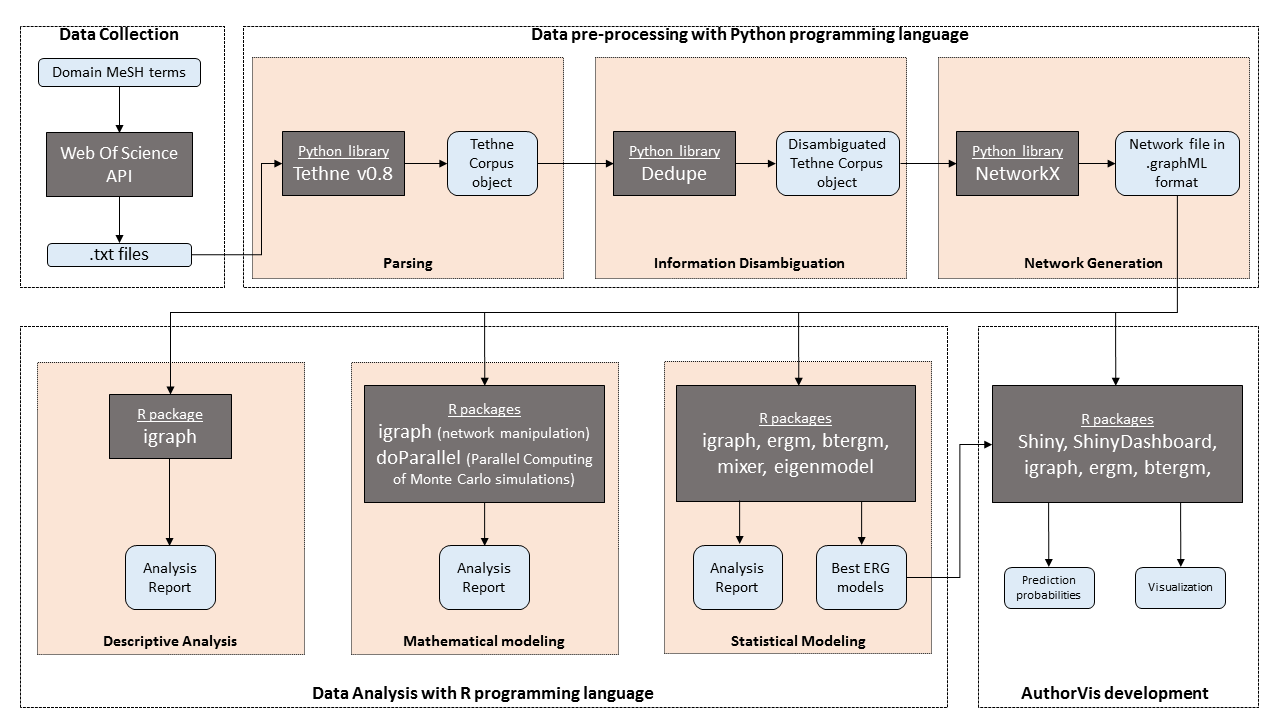
\includegraphics[scale=0.68]{Chapters/method_diagram}
%\end{sidewaysfigure}
\caption{Methodology Workflow}
\label{method_overview}
%\end{figure}
\end{sidewaysfigure}

\section{Data Collection}
\label{sec:data_collection}
Our research utilized secondary data collection techniques using the systematic literature search. We collected publication records indexed in the Thompson's Institute for Scientific Information Web Of Science (formerly known as the Web of Knowledge). %The search was conducted on papers published by Beninese authors, or papers published about Malaria, TB and HIV/AIDS involving authors affiliated to Beninese research institutions. Peer-reviewed articles were selected from systematic bibliographic search on papers indexed in Thompson's Institute for Scientific Information Web of Science (WOS) (formerly known as the Web of Knowledge). 
For each disease domain, we searched the WOS databases using combinations of disease related MeSH terms. For the malaria research domain, we combined the following MeSH terms: "Malaria", "Anopheles", "Plasmodium" and "vector". The HIV/AIDS  related MeSH terms are "HIV", "AIDS", "VIH", and "HIV infections". The TB related MeSH terms include "Tuberculosis", "Mycobacterium", and "Infection". We restricted the search to the period from 1996 to 2016 and to "Benin" for country. We manually screened the records in order to only select those published by Beninese authors, or papers published on each disease domain involving at least one author affiliated to a Beninese research institution. No restriction was placed upon the document types. For each disease domain, we first queried the WOS with each MeSH term independently, then combined the other terms so the query return the maximum number of results. The Full citations information containing the authors' names, their institutional affiliations, the year of publication, as well as the number of times the document was cited were recorded as bibliographic text files. After a second manual screening, only records that met the above listed inclusion criteria were finally selected. The selected records were saved in bibliographic text files and input to parser and functions for disambiguating the names of authors and other entities such as cities or research facilities.

\subsection{Parsing and Information Disambiguation}
\label{sec:meth_and}
%From each search domain, the bibliographic text files were parsed using Tethne v0.8 \cite{peirson_tethne_2016}, a python library for parsing bibliographic data. Tethne generated a bibliographic corpus object which is processed for information disambiguation.\\
%One common challenge in processing bibliometric data is the matching problem. Multiple names can refer to the same author. A well-known approach to solving this issue is termed as Author Name Disambiguation (AND). While many AND methods have been reported in the literature \cite{ferreira_brief_2012,giles_name_2005}, we chose to apply a fuzzy matching machine learning technique of AND. 
We used Dedupe, a python library (obtained from \url{https://github.com/datamade/dedupe}) to disambiguate authors' names and assign a unique identification number to each author. We manually annotated 10\% of the names and then trained the algorithm to automatically disambiguate the remaining of the entries. Dedupe is interactive and adjusts further annotations as the disambiguation process evolves. 
%Dedupe is based on the work of Bilenko \cite{bilenko_learnable_2006} and has been developed by Gregg Forest and Derek Eder. For more information on Dedupe, we refer the reader to the authors' Github repository available at \url{https://github.com/datamade/dedupe}.
We evaluated our AND fuzzy matching machine learning method by computing Precision and recall metrics. Dedupe was also used to normalize and disambiguate other information such as research center affiliations, city, and country. At the end of the Information Disambiguation process, a disambiguated Tethne corpus object was generated and used as input to the co-authorship network generation processing.
%The concept of AND has been extended to also disambiguate institution affiliation names and journal names. 


\subsection{Network Generation}
Using NetworkX \cite{schult_exploring_2008}, another python library, we wrote a script taking the disambiguated Tethne corpus object as input to generate undirected multigraph co-authorship networks containing parallel edges. Each author or researcher from the disambiguated Tethne corpus represented a vertex. An edge was created between two authors (vertices) when they author a document together. Multiple parallel edges were created between two authors when they coauthor multiple papers together. Our script output NetworkX graph objects where vertices were defined by several attributes including name, affiliation, city, country, number of publication and total number of times cited. Edges had attributes associated with them such as a unique identifier, the number of times a pair of authors was cited and the number of publications of a pair of authors. The undirected multigraph networkX objects were finally exported as .graphML files and used as input for data analyses.

%\section{Data Analysis}
\section{Descriptive Data Analysis}
For each co-authorship network, the numbers of authors, edges, and publications are plotted against the co-authorship years span. Using \textbf{igraph}, a network analysis package developed in R, each of the graphML files is converted into an igraph network object. For the descriptive analysis, we use the \textbf{igraph} package to compute the vertex degree and examined the degree distribution using both the natural frequency and the log scale degree distribution to characterize the type of distribution. We also computed vertex closeness, betweenness, eigenvector centrality measures and edge betweenness centrality measures to respectively identify the top 10 most connected authors, the top 10 broker authors, the top 10 network hubs, and the top 10 most important edges for information flow.  % and dyadic centrality measures:

%\begin{itemize}
%\item Degree of the vertices in the network defined as the number of ties to a given author. After converting the multigraph network in a weighted graph where weights are the number of authorship between two authors, the strength of the vertices was also computed.
%\item Betweenness: it is the number of shortest paths between alters that go through a particular author. It relates to the perspective that importance relates to where a vertex is located with respect to the paths in the network graph. According to Freeman \cite{freeman_set_1977}, it is defined as:
%\begin{equation} 
%c_{B}(v)=\frac{\sigma (s,t|v)}{\sum_{s \neq t \neq v \in V}\sigma (s,t)} 
%\end{equation} where $\sigma(s,t|v)$ is the total number of shortest paths between vertices $s$ and $t$ that pass through vertex $v$, and $\sigma (s,t)$ is the total number of shortest paths between $s$ and $t$ regardless of whether or not they pass through $v$.
%\item Closeness: the number of steps required for a particular author to access every other authors in the network. It captures the notion that a vertex is central if it is close to many other vertices. Considering a network $G=(V,E)$ where $V$ is the set of vertices and $E$, the set of edges, the closeness centrality $c_{Cl}(v)$ of a vertex $v$ is defined as:
%\begin{equation} c_{Cl}(v)=\frac{1}{\sum_{u\in V}dist(v,u)} \end{equation} where $dist(v,u)$ is defined as the geodesic distance between the vertices $u,v \in V$.
%\item Eigenvectors: degree to which an author is connected to other well connected authors in the network. It seeks to capture the idea that the more central the neighbors of a vertex are, the more central that vertex itself is. According to Bonacich \cite{bonacich_factoring_1972} and Katz \cite{katz_new_1953}, the Eigenvector centrality measure is defined as:
%\begin{equation} c_{E_i}(v)=\alpha \sum_{\{u,v\}\in E}c_{E_i}(u) \end{equation} Where the vector $\mathbf{c}_{E_i}=(c_{E_i}(1),\dots ,c_{E_i}(N_v))^T$ is the solution to the eigenvalue problem $\mathbf{Ac}_{E_i}=\alpha^{-1}\mathbf{c}_{E_i}$, where $\mathbf{A}$ is the adjacency matrix for the network $G$. According to Bonacich \cite{bonacich_factoring_1972}, an optimal choice of $\alpha^{-1}$ is the largest eigenvalue of $\mathbf{A}$
%\item Brokerage: degree to which an actor occupies a brokerage position across all pairs of alters.
%\item Edge betweenness centrality extends from the notion of vertex centrality. It reflects the number of shortest paths traversing that edge. This centrality measure was computed to assess which co-authorship collaboration ties are important for the flow of information.
%\end{itemize}

\subsection{Characterizing Network cohesion}
The extent to which subsets of authors are cohesive with respect to their relation in the co-authorship network was assessed through network cohesion. Specifically, we determined if collaborators (co-authors) of a given author tend to collaborate as well, and what subset of collaborating authors tend to be more productive in the network. 
%While there are many techniques to determine network cohesion \citep{kolaczyk_statistical_2014}, 
Using the \textbf{igraph} package, we conducted clique detection by computing the maximal cliques and their sizes, the density, and the transitivity. We also conducted a census of the connected components in each network, identify the giant component and characterize its size. Cut vertices were also computed to list the weak articulation points of each network. \\
The agglomerative hierarchical clustering method was used to identify clusters (or research communities) in the network. 
%In addition, we conducted cliques detection and clustering or communities detection on each network. 
Finally, we generated a visualization of each co-authorship network weighting the vertex size by their betweenness values and assigning colors based on their cluster membership determined by the hierarchical clustering method.
%\begin{itemize}
%\item Cliques: According to Kolaczyk and Cs\'ardi \cite{kolaczyk_statistical_2014}, cliques are defined as complete subgraphs such that all vertices within the subset are connected by edges. We computed the number of maximal cliques and assessed their size.
%\item Density: Defined as the frequency of realized edges relative to potential edges, the density of a subgraph $H$ in $G$ provides a measure of how close $H$ is to be a clique in $G$. Density values vary between 0 and 1:
%\begin{equation} 
%den(H)=\frac{|E_H|}{|V_H|(V_H-1)/2} 
%\end{equation}
%
%\item Relative frequency: we assess the relative frequency of $G$ by computing its transitivity defined as: 
%\begin{equation} 
%cl_T = \frac{3\tau_\Delta (G)}{\tau_3 (G)} 
%\end{equation}
%where $\tau_\Delta (G)$ is the number of triangles in $G$, and $\tau_3 (G)$ is the number of connected triples (sometimes referred to as 2-star). This measure is also referred to as the fraction of transitive triples. It represents a measure of global clustering of $G$ summarizing the relative frequency with which connected triples close to form triangles \cite{kolaczyk_statistical_2014}.
%\item Connectivity, Cuts, and Flows: We investigated the concepts of vertex and edge cuts derived from the concept of vertex (edge) connectivity. The vertex (edge) connectivity of a graph $G$ is the largest integer such that $G$ is k-vertex- (edge-) connected \cite{kolaczyk_statistical_2014}. These measures helped assess the most important authors for information flow and the long-term sustainability of each network. Since co-authorship networks are undirected graphs, the concept of weak and strong connectivity was irrelevant. A graph $G$ is said to be connected if every vertex in $G$ is reachable from every other vertex. Usually, one of the connected components can dominate the others, hence the concept of giant component.
%\item Graph Partitioning: Regularly framed as community detection problem, we applied graph partitioning to find subsets of vertices that demonstrate a 'cohesiveness' with respect to their underlying relational patterns. Cohesive subsets of vertices generally are well connected among themselves and are well separated from the other vertices in the graph. Two established methods of graph partitioning are Hierarchical clustering (agglomerative vs divisive) and Spectral clustering \cite{kolaczyk_statistical_2014}. In our research, we applied agglomerative Hierarchical Clustering to the co-authorship networks.
%\end{itemize}
\pagebreak
\section{Modeling of Network Data}
%The purposes of network graph modeling are to test significance of the characteristics of observed network graphs, and to study proposed mechanisms of real-world networks such as degree distributions and small-world effects \cite{kolaczyk_statistical_2014}. A model for a network graph is a collection of possible graphs $\mathscr{G}$ with a probability distribution $\mathbb{P}_\theta$ defined as:
%\begin{equation} 
%\{ \mathbb{P}_\theta\ (G), G \in \mathscr{G} : \theta \in \Theta \} 
%\end{equation}
%where $\theta$ is a vector of parameters ranging over values in $\Theta$.\\
%Given an observed co-authorship network graph $G^{obs}$ and some structural characteristics $\eta (\cdot)$, our goal is to assess if $\eta (G^{obs})$ is unusual. We then compare $\eta (G^{obs})$ to collection of values $\{\eta(G):G \in \mathscr{G}\}$. If $\eta (G^{obs})$ is too extreme with respect to this collection, then we have enough evidence to assert that $\eta (G^{obs})$ is not a uniform draw from $\mathscr{G}$.\\
%Given the computationally expensive calculations involved in modeling in general, and the expected large size of our network, we parallelized all processing.

\subsection{Mathematical Modeling}
%We used the characteristics of each observed network as input to the \textbf{igraph} package to simulate 1,000 networks from all four mathematical models for network graphs:
%\begin{itemize}
%\item Classical Random Graph Models: First established by Erd\H os and R\'enyi \cite{erdos_random_1959,erdos_evolution_1960,erdos_strength_1964}, it specifies a collection of graphs $\mathscr{G}$ with a uniform probability $\mathbb{P}(\cdot)$ over $\mathscr{G}$. A variant of this model called the Bernoulli Random Graph Model was also defined by Gilbert \cite{gilbert_random_1959}.
%\item Generalized Random Graph Models: These models emanated from the generalization of Erd\H os and R\'enyi's formulation, defining a collection of graphs $\mathscr{G}$ with prespecified degree sequence.
%\item Mechanistic Network Graph Models: These models mimic real-world phenomena and include Small-World Models commonly referred to as "six-degree separation". It was introduced by Watts and Strogatz \cite{watts_collective_1998} and have since received a lot of interests in the existing literature especially in Neuroscience. Small-world networks usually exhibit high levels of clustering and small distances between vertices. Classical models are not fit to better represent such behaviors since they usually display low levels of clustering and small distance between vertices. Examples of known small-world networks include the network of connected proteins  or the transcriptional networks of genes \cite{van_noort_yeast_2004}. A variant of Small-World models is the Preferential Attachment Models defined based on the popular principle of "the rich get richer". Preferential attachment models gained fascination after the work of Barab\'asi and Albert who studied the growth of the World Wide Web \cite{barabasi_emergence_1999}. Examples of Preferential Attachment networks include that of the World Wide Web and the scientific citation network \cite{albert_internet:_1999,jeong_measuring_2003}. An important characteristic of these models is that as time tend to infinity, there degree distribution tends to follow a power law.
%\end{itemize}
We input the observed characteristics of each co-authorship network to an \textbf{igraph} function to perform $1,000$ Monte-Carlo based simulations of the four different mathematical models for network graphs (Classical Random Graph, Generalized Random Graph, Watts-Strogatz Small-World, and the Barab\'asi-Albert Preferential Attachment) presented in section \ref{sec:back_mathModel}. We assessed the significance of the observed characteristics by comparing them to those of the $1,000$ simulated networks using a one sample Student’s t-test. Characteristics we assessed significance for are the average shortest paths, the clustering coefficient and the number of communities detected by the hierarchical clustering methods.

\subsection{Statistical Modeling}
%Although mathematical models tend to be simpler than statistical models, the latter allow model fitting and assessment. 
To model the complexity of the structure of each co-authorship network, we fit the SBM, the ERGM, the TERGM, and the LNM (presented in section \ref{sec:back_statModel}) to each co-authorship network data. 
For each model, we computed and included in the model an important social network principle referred to as homophily which is defined in our network as the tendency of similar authors to collaborate. Another very important social network principle we also computed and included in the model, is the one of structural equivalence which is the similarity of network positions on the formation of collaboration ties in a given network. 
%We hypothesized that tie formation in each co-authorship network (i) is dependent on certain authors' characteristics,  (ii) is dependent on the concept of distance in latent space, and (iii) collaboration type and/or membership to a certain research community or class determines collaboration tie formation. 
We used the results from the static and temporal statistical network models listed above to verify the hypotheses in section \ref{hypotheses}. The purpose of this approach to network modeling is to unveil structural patterns driving collaboration tie formation in each co-authorship network.

\subsubsection{Stochastic Block Model}
\label{sec:methods_sbm}
%Blockmodeling is a statistical method to identify, in a given network, clusters or classes of authors that share structural characteristics \cite{lorrain_structural_1971,doreian_generalized_2004}. Each such cluster forms a position. The units within a cluster have the same or similar connection patterns. Given a graph $G=(V,E)$ and its adjacency matrix $\mathbf{Y}$, for two distinct nodes $i,j \in V$, the block model defined by Kolaczyk and Cs\'ardi \cite{kolaczyk_statistical_2014}, specifies that each element $Y_{ij}$ of $\mathbf{Y}$ is conditional on the class label $q$ and $r$ of the vertices $i$ and $j$. The model has the form:
%\begin{equation}Pr(\mathbf{Y}=\mathbf{y})=\left( \frac{1}{\kappa} \right) exp \set*{ \sum_{q,r} \theta_{qr} L_{qr}(\mathbf{y}) }\end{equation}
%where $L_{qr}$ is the number of edges in the observed graph $\mathbf{y}$ connecting vertices of classes $q$ and $r$, $\theta_{qr}$ is the parameter estimates, and $\kappa$ is a normalization constant defined as:
%\begin{equation}
%\kappa = \sum_{\mathbf{y}}exp \set*{ \sum_{q,r} \theta_{qr} L_{qr}(\mathbf{y}) }
%\end{equation}
%Stochastic block model (SBM) originated from the ideas that equivalent units can be grouped together. There are three definitions of equivalences which are structural, automorphic and regular \cite{mali_dynamic_2012}. In practice, the differences in types of equivalence tend to blur when stochastic block modeling is applied to real networks. 
We used SBM to both model each of the observed networks but also as a model based clustering technique. After fitting the SBM, we examined the posterior probability of class membership from the returned object. We then determined the class membership of each vertex class assignment based on the maximum a posteriori criterion. Class membership was added to the network as an additional nodal attribute. Subroutines of R package \textbf{mixer} \citep{Daudinmixturemodelrandom2008,ZanghiFastonlinegraph2008,ZanghiStrategiesonlineinference2010,LatoucheVariationalBayesianinference2012} was used to fit and evaluate the SBM. \textbf{Mixer} used the Integration Classification Likelihood (ICL) criterion to select the number of classes fit to the observed network. We finally examined the summary plot generated by the \textbf{Mixer} package which contains the ICL, the degree distribution, the reorganized adjacency matrix, and the inter/intra class probability plots. While the ICL plot displays the optimal number of classes, the degree distribution helps assess the goodness-of-fit of the SBM to the observed data. The reorganized adjacency matrix plot shows the interactions between the classes of the network and the inter/intra class probabilities plot highlights the inter and intra interactions between the detected classes.
%
%\subsubsection{Dynamic Stochastic Block Model}
%\label{sec:methods_dynsbm}
%The Dynamic Stochastic Block Model (dynSBM) emerged from the recent interests in statistical modeling of dynamic or temporal networks \cite{xu_dynamic_2014}. It is a recent model based clustering approach to dynamically evolving or longitudinal networks \cite{matias_statistical_2016,hutchison_dynamic_2013,xu_dynamic_2014}. We refer the reader to the work of Matias and Miele \cite{matias_statistical_2016} in their 2016 paper for a thorough model definition.\\ 
%The dynSBM method is a combination of Stochastic Block Model (SBM) \cite{kolaczyk_statistical_2009} described in section \ref{sec:methods_sbm} for the static aspect and independent Markov chains for the temporal evolution of the network. The main focus of this method is on nodes classification or the task of community detection. The dynSBM method allows the modeling of sequence of different snapshots of temporal or dynamic networks. In a different paper, the method was used to unveil the dynamic structure of different ecologic networks of colonies of ants or a community of Broadstone Stream \cite{miele_revealing_2017}. The model is suited for discrete time in dynamic networks. We used dynSBM to investigate research group switching across the investigation period, and map the dynamic of collaborative research among the identified research groups. We presented an alluvial plot representing a map of the co-authorship patterns, group switching within time. The R package \textbf{dynSBM} \cite{matias_statistical_2016} was used to fit the dynSBM. Matias and Miele \cite{matias_statistical_2016} assert that the number of groups can be selected statistically using the Integration Classification Likelihood (ICL) criterion or the "elbow" heuristic. The optimum number of groups therefore corresponds to the highest ICL. As per the "elbow" heuristic, the optimum number of groups corresponds to the point where the slope of the log-likelihood decreases significantly. In this thesis, we used both the ICL and the "elbow" heuristic to select the number of groups in the final dynSBM model. We defined the selected number of detected groups in the final model as the minimum of the number of detected groups determined by the ICL criterion and the "elbow" heuristic.

\subsubsection{Exponential Random Graph Model}
\label{sec:methods_ergm}
%Also referred to as p* models, Exponential Random Graph Models (ERGMs) are probability models for network designed in analogy to Generalized Linear Models (GLMs) \cite{kolaczyk_statistical_2014}. ERGMs have gain increasing interests especially in modeling social networks. Robins et al. \cite{robins_introduction_2007} provides a nice introduction to ERGM as well as a general framework for ERGM creation which we closely followed here. 
The R package \textbf{ergm} \cite{HandcockERGMFitsimulate2003,HunterergmPackageFit2008} was used to fit ERGM to the observed networks. We used ERGM to model the network ties, the dependent variable as a function of nodal and dyadic attributes (covariates) such as the number of times an author was cited, the number of publications, the number of collaborators, the collaboration type as well as its community membership as determined by the SBM. \\
%investigate how local processes affect collaboration tie formation between authors. We 
Given the high transitivity coefficient of this network, we also included transitivity as a network structural process. As recommended for ERGM model specification for undirected network, we investigated homophily which is the tendency of similar author to collaborate. We also included factor attribute effect in the model. \\
%Given a random graph $G=(V,E)$, for two distinct nodes $i,j \in V$, we define a random binary variable $Y_{ij}$ such that $Y_{ij}=1$ if there is an edge $e \in E$ between $i$ and $j$, and $Y_{ij}=0$ otherwise. Since co-authorship networks are by definition undirected networks, $Y_{ij}=Y_{ji}$ and the matrix $\mathbf{Y}=\left[Y_{ij}\right]$ represents the random adjacency matrix for $G$. The general formulation of ERGM is therefore:
%\begin{equation}
%Pr(\mathbf{Y}=\mathbf{y})=\left( \frac{1}{\kappa} \right) exp \set*{ \sum_{H} \theta_H g_H(\mathbf{y})}
%\end{equation}
%where each $H$ is a configuration, a set of possible edges among a subset of the vertices in $G$ and $g_H(\mathbf{y})=\prod_{y_{ij} \in H}y_{ij}$ is the network statistic corresponding to the configuration $H$; $g_H(\mathbf{y})=1$ if the configuration is observed in the network $\mathbf{y}$, and is $0$ otherwise. $\theta_H$ is the parameter corresponding to the configuration $H$ (and is non-zero only if all pairs of variables in $H$ are assumed to be conditionally dependent); $\kappa$ is a normalization constant defined as:
%\begin{equation}
%\kappa = \sum_{\mathbf{y}}exp \set*{ \sum_{H} \theta_H g_H(\mathbf{y})}
%\end{equation}.\\
Several models containing nodal, dyadic and structural terms were fit to the observed network data. The first model we fit is a naive model containing only the ERGM "edge" term. This model is nothing but the Bernoulli random graph model \cite{erdos_random_1959}. We then fit another model containing only nodal and/or dyadic terms. Third, we fit a structural model containing only high-order terms representing network statistics such as triangles, k-stars, geometrically weighted edge-wise shared partner distribution and many more \cite{kolaczyk_statistical_2014,robins_introduction_2007}. \\
%Ideally, we expect the best model to contain nodal and dyadic covariates as well as high order ERGM terms. 
Model log-likelihood, the Akaike's Information (AIC) and the Bayesian Information (BIC) criteria were used to select the best ERGM. The best model was selected based on the lowest AIC, or the lowest BIC, and the highest log-likelihood. Usually, AIC and BIC decrease or increase together. In case of conflicting trend in AIC and BIC values, the log-likelihood was used to select the best model. We checked for model diagnostics by computing and inspecting the Goodness-Of-Fit visualization for the best model using a subroutine of the \textbf{ergm} package. %generated whenever necessay, we finally evaluated the best model (lowest AIC or BIC and highest likelihood) by assessing its goodness-of-fit to the observed network. 
A maximum of 1,000 iterations and 1,000 simulations was set as parameters to the ERGMs.

\subsubsection{Temporal Exponential Random Graph Model}
\label{sec:methods_tergm}
All Temporal Exponential Random Graph Models (TERGMs) were fit using the Markov Chain Monte Carlo Maximum Likelihood Estimation (MCMC-MLE) implemented in the \textbf{btergm} R package \cite{leifeld_temporal_2015}. 
%The Temporal Exponential Random Graph Model (TERGM) is an extension of the ERGM described in section \ref{sec:methods_ergm} proposed by Hanneke, Fu, and Xing \cite{hanneke_discrete_2010} from the work of Robins and Pattison \cite{robins_random_2001}. The TERGM was designed with the idea of accounting for inter-temporal dependence in longitudinally collected network data. TERGM was applied to each co-authorship network following from the work of Leifeld, Cranmer, and Desmarais \cite{leifeld_temporal_2015}. For a full description of the TERGM, we refer the reader to Leifeld, Cranmer, and Desmarais \cite{leifeld_temporal_2015}. \\
%Each network is subset in different temporal snapshots. In general, when the temporal network is overly dense or sparse early on or in later time periods, the TERGM tends to fit different time spans differently \cite{leifeld_temporal_2015}. To avoid such an issue, the cumulative network was subset in a certain way that balanced the number of edges across the years. 
%This strategy improved the robustness and convergence of our models. %--->this goes to the discussion
We divided each network in different snapshots spanning different intervals of time using a manual process such that the temporal snapshots are not overly dense or sparse early on or in later time periods. We used \textbf{igraph} to visualize and manually verified that the temporal snapshots are balanced across the time periods. We then modeled the network ties, the dependent variable as a function of nodal and dyadic variables. Dyadic stability and delay reciprocity memory TERGM terms were also included in the model. To check whether there is a linear trend in collaboration tie formation, we also included a linear time covariate in the model. We accounted for network structural predictors and homophily on the type of collaboration.  Model log-likelihood, the Akaike's Information (AIC) and the Bayesian Information (BIC) criteria were used to select the best TERGM corresponding to the lowest AIC or BIC, and highest log-likelihood. AIC and BIC are estimates of a function of the posterior probability of a model being true. Under a Bayesian setup, a lower BIC or AIC means that a model is more likely to be the true model.  \\
To evaluate the extent to which the final model captures the endogenous properties and processes of the observed network, we assessed model diagnostics, by inspecting the within-sample and out-of-sample goodness-of-fit visualization computed from a subroutine of the \textbf{btergm} package. For the out-of-sample goodness-of-fit, we estimated the model on the first network snapshots leaving out the last network snapshot in the series. We simulated $1,000$ networks from the model and assessed how the simulated networks predicted the left out network. As described by Desmarais and Cranmer \cite{desmarais_micro-level_2012}, we also provided a micro-interpretation of the final TERGM.

\subsubsection{Latent Network Model}
\label{sec:methods_lnm}
%Designed in analogy to Mixed Models, Latent Network Models (LNM) allow the incorporation of latent or unobserved variables in network modeling. These models specifically account for structural equivalence, to model hidden factors or information not available in the network. Kolaczyk and Cs\'ardi \cite{kolaczyk_statistical_2014} provide a formulation of LNM. Given the adjacency matrix $\mathbf{Y}$ of a graph $G=(V,E)$, for each element $Y_{ij}$ of $\mathbf{Y}$, the latent variable model is of the form:
%\begin{equation}Y_{ij}=h(\theta,z_i,z_j,\epsilon_{ij})\end{equation} where $\theta$ is a constant, the $\epsilon_{ij}$ are independent and identically distributed pair-specific effects, and $h$ is a symmetric function. The model assumes that each vertex $i\in V$ has a latent variable $z_i$. Considering observed covariates $\mathbf{Z}$, the probability of forming an edge between two nodes $i$ and $j$ ($i,j \in V$) is independent of all other vertex pairs given values of latent variables, and is defined as:
%\begin{equation}
%Pr(\mathbf{Y}|\mathbf{Z},\theta)=\prod_{i\neq j}Pr\left(Y_{ij}|z_i,z_j,\theta \right)
%\end{equation}
Hoff \cite{hoff_modeling_2008} suggested an approach based upon the principles of eigen-analysis of specifying latent variables which we followed in this dissertation. The R package \textbf{eigenmodel} developed by Hoff \cite{hoff_eigenmodel:_2012} was used to fit the LNM to the observed networks. We fit LNM with both no pair-specific and pair-specific covariates such as the type of collaboration and community assignment from the SBM. The rationale of fitting the pair-specific models with those two variables is supported by our third hypothesis which states that collaboration ties in each co-authorship network are driven by homophily in terms of community membership and/or collaboration type. We also fit other pair-specific covariates model using nodal and dyadic covariates. We visualized and compared the co-authorship network using 3 dimensional layouts determined according to the inferred latent eigenvectors in each model. Finally, we used a 5-fold cross-validation method to assess the goodness-of-fit of each model which we compared using ROC curves via the R package \textbf{ROCR} \citep{SingROCRvisualizingclassifier2005}.\\
~\\
The creation of the co-authorship tool is presented in Chapter \ref{chap_authorvis}.


%\section{Research Collaboration Ties Prediction}
%Collaboration recommendation has already been identified as valuable for interdisciplinary research, encouraging joint research and cross-domain collaboration efforts \cite{tang_cross-domain_2012,trujillo_collaboration_2010}. Often, such collaborations are hard to researchers to establish. Link prediction effectively addresses the issue of link recommendation as one of the network topology inference questions. The link prediction question as formalized by Liben-Nowell and Kleinberg \cite{liben-nowell_link-prediction_2007} seeks to infer new future interactions among members of a social network given a snapshot of such network. After developing and proposing several approaches to the link prediction question, their first application was on large co-authorship networks. Unlike many other networks, co-authorship networks are dynamic in nature. New authors can make their apparition in the network while old authors may disappear. New authorship collaborations may be initiated while old ones may stop.\\
%The many approaches to the link prediction problem can be classified in three main techniques: (i) Node neighborhood, (ii) Path based technique, and (iii) Distance based technique \cite{sharma_link_2014}. Different predictors defined each of those link prediction techniques. For example, Jaccard-coefficient, Adamic-Adar and preferential attachment are node neighborhood predictors while examples of path based predictors are Katz, and rooted PageRank.\\ 
%We used Linkpred, an easy link prediction tool written in Python and available at \url{https://github.com/rafguns/linkpred}. Our choice of this tool is motivated by the fact it is based on machine learning and uses a wide range of global, local and distance based predictors.
%Our goal was to predict future co-authorship links in 5 and 2 years based on the observed collaboration over a 20 years of research collaboration. We therefore split each network data in a training set and a test set. Prediction models were trained on the training set and evaluated on the test set. In the 5-year link prediction question, we inferred new collaborations between authors in the next 5 years. Hence, our training set covered the first 15 years and the test set, the next 5 years. Similarly, for the 2-year link prediction question, we split the data in a training set covering the first 18 years and a test set of the next 2 years for evaluation purposes.\\
%The Receiver Operating Curve (ROC), the Area Under the Curve (AUC), precision, recall and F-measures were used as evaluation metrics.
 % Malaria Co-authorship Network

%*******10********20********30********40********50********60********70********80

% For all chapters, use the newdefined chap{} instead of chapter{}
% This will make the text at the top-left of the page be the same as the chapter

\chap{Results: The Malaria Co-authorship Network}
\label{chap:malaria}
%\section{Background}
%Malaria remains one of the three major public health concerns in Sub Saharan Africa where it affects millions of people and impact negatively on their socioeconomic life \cite{davis_emerging_2001}. In the Millenium Declaration, Malaria has been given a special attention in terms of the successful achievement of the $6^{th}$ development goal of the Millenium Challenge \cite{assembly_united_2000}. In the Republic of Benin, initiatives such as the US President's Malaria Initiative have supported governmental and non-governmental organizations to reduce the mortality and morbidity related to Malaria \cite{arthur_institute_2014,stoops_presidents_2008}. With these financial supports at hand, such efforts in Benin have led to a sharp increase in public health interventions and many positive public health outcomes in terms of the reduction of mortality and morbidity related to Malaria \cite{barat_four_2006}. Such increase in public health interventions translated in the successful implementation and sustainability of entomological surveillance of malaria for more than six years since 2008 \cite{akogbeto_six_2015}. Between the years 2000 and 2009, the increase in funding led to an annual decrease of 5.2\% in the incidence of malaria and 5.3\% in malaria-related deaths \cite{world_health_organization_world_2012}. This encouraging success stories have even motivated other authors to enunciate the ambitious malaria eradication plan \cite{alonso_research_2011}.\\
%Despite the progress in malaria, very little is known on the dynamics of the malaria research collaboration network. This situation results in a lack of information on the main players and drivers of the progress made. As for the eradication of chickenpox \cite{jamison_disease_2006}, collaborative research will undoubtedly play an important role in the successful attainment of the malaria eradication plan in Subsaharan Africa in general and in Benin particularly. By collaborting with each other, researchers form continuous and sustainable collaboration through intensive network practices that go beyond the regional boundaries \cite{newman_structure_2001}. In addition, the fact that the extensive research conducted has not prevented malaria from outpacing the proposed solutions is a definitive clue to investigating the structure of the malaria research community. Research collaboration constitutes a stable basis for the provision of evidence based information in the formulation of fundamental principles and guidelines for the elaboration of public health strategies. \\%Therefore, we propose in this study, to document, describe and analyze the different aspects of the malaria research collaboration in the Republic of Benin.\\
%Understanding the structure of this network is capital since it can help improve research prioritization \cite{ghafouri_social_2014}, identify prolific researchers, better design, strategic planning and implementation of research programs \cite{morel_co-authorship_2009}, and promote cooperation and translational research initiatives \cite{gonzalez-alcaide_scientific_2012}.% We choose a social network analysis approach which will reveal undiscovered knowledge on effort of researchers in working together towards the reduction of the burden of Malaria in Benin.% \\
%In the first section of this chapter, we present the results of the descriptive Network analysis and the mathematical modeling of the Malaria co-authorship network. In the last section, we the results of the statistical modeling are presented. We hypothesized that tie formation in the Malaria co-authorship network (i) is dependent on certain authors' characteristics,  (ii) is dependent on the concept of distance in latent space, and (iii) collaboration type and/or membership to a certain research community or class determines collaboration tie formation.

\section{Data}
\label{sec:malaria_data}
%The data collection was carried on papers indexed in Thompson's Institute for Scientific Information Web Of Science (formerly known as the Web of Knowledge). 
The search was conducted using combinations of Malaria related MeSH terms including "malaria", "Anopheles", "Plasmodium" and "vector". %We restricted the search to the period from 1996 to 2016 and to "Benin" for country. We further screened the papers in order to only select those published by Beninese authors, or papers published on Malaria involving at least one author affiliated to a Beninese research institution. No restriction was placed upon the document types.  We first started querying with each term independently, we then combined the other terms so the query return the maximum number of results. The  Full citations information containing the authors' names, their institutional affiliations, the year of publication, as well as the number of times the document was cited were recorded as a bibliographic corpus in text format. After a second screening only research that have met the above listed inclusion criteria and that were published between January 1, 1996 and December 31, 2016 were selected in this study.\\
The final query set (Table \ref{table: malaria_search}) returned 685 records. After screening, 424 documents met the selection criteria. On average, there was 10.67 authors per published document.\\
After the Author Name Disambiguation, we identified 1792 unique authors with a precision of 99.87\% and a recall of 95.46\%. The generated multigraph co-authorship network therefore contained 1792 vertices (authors) and 116,388 parallel edges (collaborations).\\
%For the temporal or dynamic models, we subset the network in different temporal snapshots. We created the snapshots in a certain way that balanced the number of edges across the years. Such an uneven subsetting improved the robustness of our models and ensured model convergence. We ended up with 7 snapshots representing respectively the following timestamps: 1996 -- 2006, 2007 -- 2009, 2010 -- 2011, 2012 -- 2013, 2014, 2015 and 2016. %Each vertex (author) in the network has 2 attributes: name and a unique identification number. Each edge has 8 attributes: key, subject, abstract, year, wosid (Web of science Identification number), journal, title and doi (digital identifier object).

\begin{table}[!ht]
\caption{Malaria Bibliographic Search Queries.}
\label{table: malaria_search}
\centering
%\hspace*{-0.5cm}
\small
\begin{tabular}{llc}
\toprule
Set & \multicolumn{1}{c}{Queries} & Results \\
\midrule
\#1 & \begin{tabular}[c]{@{}l@{}}TOPIC: (malaria) OR TOPIC: (mosquito),\\Refined by: COUNTRIES/TERRITORIES: (BENIN)\end{tabular} & 513 \\\\
\#2 & \begin{tabular}[c]{@{}l@{}}TOPIC: (malaria) OR TOPIC: (mosquito) OR TOPIC: (anopheles),\\Refined by: COUNTRIES/TERRITORIES: (BENIN)\end{tabular} & 529 \\\\
\#3 & \begin{tabular}[c]{@{}l@{}}TOPIC: (malaria) OR TOPIC: (mosquito) OR TOPIC: (anopheles) \\OR TOPIC: (plasmodium) OR TOPIC: (bednet),\\Refined by: COUNTRIES/TERRITORIES: (BENIN)\end{tabular} & 544 \\\\
\#4 & \begin{tabular}[c]{@{}l@{}}TOPIC: (malaria) OR TOPIC: (mosquito) OR TOPIC: (anopheles)\\ OR TOPIC: (plasmodium) OR TOPIC: (net) OR TOPIC: (vector),\\Refined by: COUNTRIES/TERRITORIES: (BENIN)\end{tabular} & 685 \\
\midrule
Final Set & \#1 OR \#2 OR \#3 OR \#4 & 685\\
\bottomrule
\end{tabular}%}
\end{table}

The evolution of the published Malaria related documents, authors and collaborations from January 1996 to December 2016 is presented on figure \ref{fig: malaria_pubDist}.

\begin{figure}[!ht]
\centering
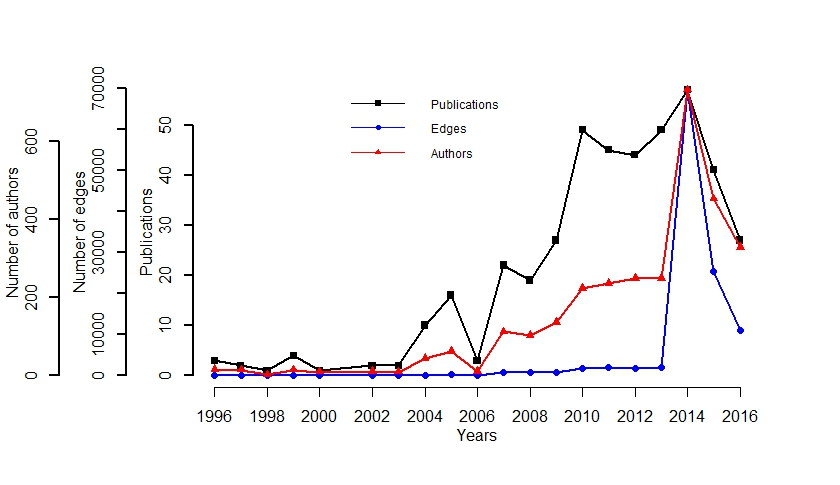
\includegraphics[scale=0.65]{Chapters/malaria/pubDist}
\caption{Evolution of the published Malaria related documents, authors and collaborations from January 1996 to December 2016}
\label{fig: malaria_pubDist}
\end{figure}

\section{Descriptive Data Analysis}
\label{sec:malaria_descstat}
The degrees of the multigraph network range between 1 and 1338 with an average degree distribution of 106.46. We noted in addition, a substantial number of vertices with low degrees (Fig. \ref{malaria_fig1}). There was also a non-trivial number of vertices with higher order of degree magnitudes. A log scale distribution of the degrees demonstrate that the vertex degrees tend to follow a heavy-tail distribution.\\
After we convert the multigraph network in a weighted graph, it results in a simple graph of 1792 vertices and 95,787 weighted edges. Mean Closeness centrality ranges between $3.118\times 10^{-7}$ and $5.152\times 10^{-6}$ with a median of $5.112\times 10^{-6}$. This measure  suggests a highly right-skewed distribution. Betweenness measures range between 0 and 245600 with a median of 1985. A network visualization with the vertices' size proportional to betweenness centrality measures clearly reveals the presence of broker authors (Table \ref{table: malaria_list}). The median eigenvectors measure is 0.005, its  mean is estimated at 0.09. Eigenvectors measures reveal the presence of multiple cluttered authors suggesting the presence of closed collaboration groups. Table \ref{table: malaria_list} presents a list of the 10 authors with the highest Eigenvectors values.

\begin{figure}[!ht]
\centering
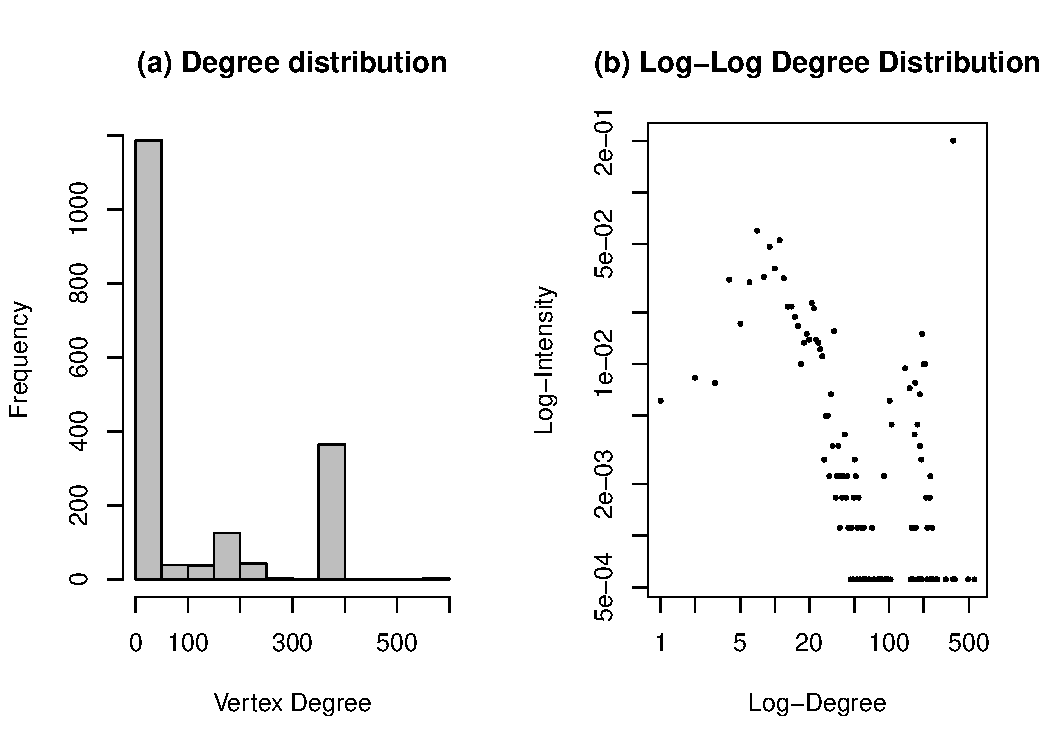
\includegraphics[scale=0.75]{Chapters/malaria/degreeDistribution}
\caption{Degree distribution of the Malaria co-authorship network}
\label{malaria_fig1}
\end{figure}

The computation of edge betweenness identifies co-authorship collaborations that are important for the flow of information. In Table \ref{table: malaria_list}, We present the top 10 most important collaborations for the flow of information in the Malaria co-authorship network in Benin.

%\pagebreak
\begin{table}[!ht]
\caption{List of the most important authors and collaborations in the Malaria co-authorship network}
\label{table: malaria_list}
\centering \scriptsize
\begin{tabular}{l}
  \toprule
\textbf{Top 10 Brokers}\\
%\hline
\hspace{20pt}MASSOUGBODJI ACHILLE\\
\hspace{20pt}HAY SIMON I\\
\hspace{20pt}KAREMA CORINE\\
\hspace{20pt}SANNI AMBALIOU\\
\hspace{20pt}KENGNE ANDRE PASCAL\\
\hspace{20pt}AKOGBETO MARTIN\\
\hspace{20pt}NDAM NICAISE TUIKUE\\
\hspace{20pt}MALIK ELFATIH M\\
\hspace{20pt}DABIRE K ROCH\\
\hspace{20pt}DELORON PHILIPPE\\
\hline
\textbf{Top 10 most connected authors (Top 10 network hubs)}\\
\hspace{20pt}MASSOUGBODJI ACHILLE\\
\hspace{20pt}KAREMA CORINE\\
\hspace{20pt}GONZALEZ RAQUEL\\
\hspace{20pt}MENENDEZ CLARA\\
\hspace{20pt}DALESSANDRO UMBERTO\\
\hspace{20pt}OGUTU BERNHARDS R\\
\hspace{20pt}FAUCHER JEANFRANCOIS\\
\hspace{20pt}BASSAT QUIQUE\\
\hspace{20pt}MARTENSSON ANDREAS\\
\hspace{20pt}HAY SIMON I\\
\hline
\textbf{Top 10 most important edges for information flow}\\
\hspace{20pt}DABIRE K ROCH -- KENGNE ANDRE PASCAL\\
\hspace{20pt}BALDET THIERRY -- KENGNE ANDRE PASCAL\\
\hspace{20pt}AKOGBETO MARTIN -- MALIK ELFATIH M\\
\hspace{20pt}AVLESSI FELICIEN -- MOUDACHIROU MANSOUROU\\
\hspace{20pt}AKOGBETO MARTIN -- AVLESSI FELICIEN\\
\hspace{20pt}MASSOUGBODJI ACHILLE -- RAHIMY MOHAMED CHERIF\\
\hspace{20pt}DIABATE ABDOULAYE -- KENGNE ANDRE PASCAL\\
\hspace{20pt}GARCIA ANDRE -- SANNI AMBALIOU\\
\hspace{20pt}KAREMA CORINE -- MALIK ELFATIH M\\      
\hspace{20pt}HAY SIMON I -- MALIK ELFATIH M\\
\hline
\textbf{Weak articulation points}\\
\hspace{20pt}NOEL VALERIE\\
\hspace{20pt}DJOGBENOU LUC\\
\hspace{20pt}ZOHOUN I\\
\hspace{20pt}SANNI AMBALIOU\\
\hspace{20pt}EDORH ALEODJRODO PATRICK\\
\hspace{20pt}ALLABI AUREL\\
\hspace{20pt}HOUNKONNOU MAHOUTON NORBERT\\
\hspace{20pt}FAYOMI BENJAMIN\\
\hspace{20pt}KINDEGAZARD DOROTHEE A\\
\hspace{20pt}DJOUAKA ROUSSEAU\\
\hspace{20pt}RAHIMY MOHAMED CHERIF\\
\hspace{20pt}BALDET THIERRY\\
\hspace{20pt}DOSSOUGBETE L\\
\hspace{20pt}GARCIA ANDRE\\
\hspace{20pt}MASSOUGBODJI ACHILLE\\
\hspace{20pt}AKOGBETO MARTIN\\
\bottomrule
\end{tabular}
\end{table}

\subsection{Network Cohesion}
A total of 365 maximal cliques are identified in the network among which 9 cliques of size 2, 14 cliques of size 3, 155 cliques of size 8, and 142 cliques of size 7. Larger maximal cliques sizes range from 102 authors to 365 authors and are all found once across the network. \\The malaria co-authorship network has a density of 0.0596 and a transitivity of 0.965 indicating that 96.5\% of the connected triples in the network are close to form triangles. The transitivity metrics is a measure of the global clustering of the network.\\The network is not connected and a census of all the connected components within the network reveals the existence of a giant component that dominates all the other connected components. This giant component includes 94\% (1686 vertices) of all the vertices in the network with none of the other components alone carrying less than 1\% of the vertices in the network (Fig. \ref{malaria_fig5}).  \\The assessment of information flow in the network via cut vertices reveal the existence of 16 authors as the most vulnerable vertices in the network. Table \ref{table: malaria_list} lists the authors that constitute the weak articulation points in the malaria co-authorship network. Cut vertices are crucial to the sustainability of networks \cite{kolaczyk_statistical_2014}.\\
The agglomerative hierarchical clustering method identifies 23 research communities (or clusters) in the network. Sizes of the clusters range between 2 and 570 with large research communities containing between 202 and 569 authors. Medium size research communities contain between 10 and 62 authors. Only 7 out of the 23 research communities identified are part of the giant component. Figure \ref{malaria_fig5} displays the giant component of the network with each different colors representing each of the 7 research communities.

\begin{figure}[!ht]
\centering
\hspace*{-1cm}
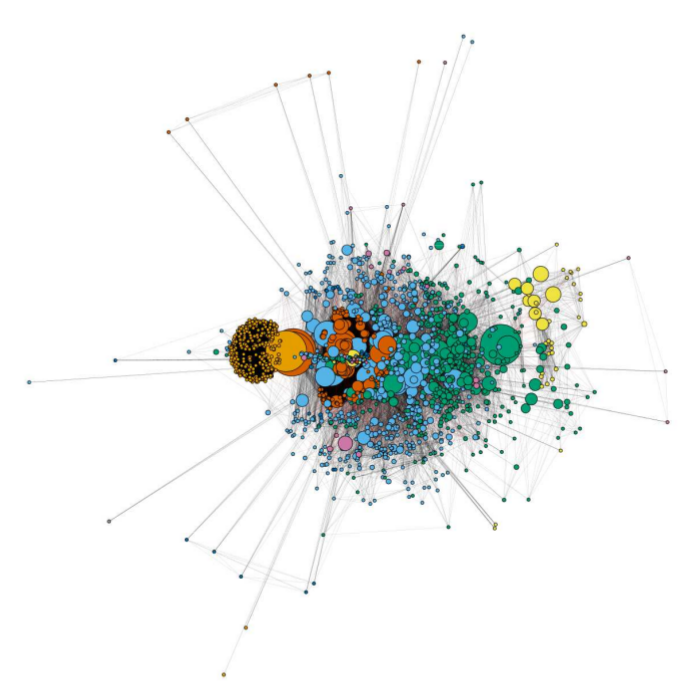
\includegraphics[scale=0.5]{Chapters/malaria/mnet}
\caption{Malaria co-authorship network -- Main component. \\Authors (vertices) of the same color belong to the same research community or cluster}
\label{malaria_fig5}
\end{figure}
\pagebreak
\section{Modeling}
\subsection{Mathematical Modeling}
The hierarchical clustering method of community detection algorithm has identified 23 different clusters/communities in the co-authorship network out of which 7 form a giant component. One of the question of interest in this section is whether the number of communities detected is expected or not. The results of 1,000 Monte Carlo based simulations to test the significance of this observed characteristic are presented on figures \ref{malaria_fig3} and \ref{malaria_fig4}. Figure \ref{malaria_fig3} clearly demonstrates that the number of communities detected is unusual from the perspective of both Classical random graphs and generalized random graphs (p-value < 0.0001). From the Classical random graph model, the expected number of communities is 3.934 (95\%CI: 3.90 -- 3.97). Similarly, the expected number of communities from the generalized random graph model is 7.501 (95\%CI: 7.39 -- 7.61).

\begin{figure}[!ht]
\centering
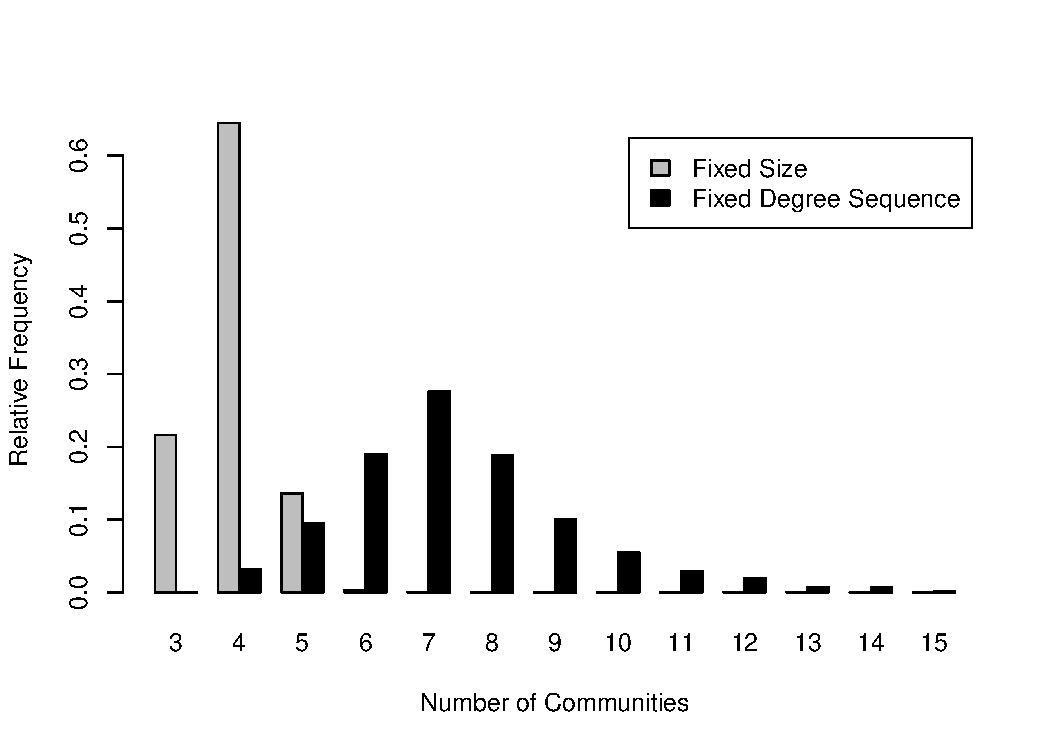
\includegraphics[scale=0.75]{Chapters/malaria/randomComm}
\caption{Monte-Carlo simulations: Number of detected communities by the random graph models}
\label{malaria_fig3}
\end{figure}

Figure \ref{malaria_fig4} displays the number of detected research communities using the Barab\'asi-Albert's preferential attachment and the Watts-Strogatz models. Supprisingly enough, the observed number of communities is also extreme per both models (p-value < 0.0001). The expected number from the Watts-Strogatz model simulations is 3.056 (95\%CI: 3.04 -- 3.07) and 45.569 (95\%CI: 45.42 -- 45.72) from the Barab\'asi-Albert model simulations.

\begin{figure}[!ht]
\centering
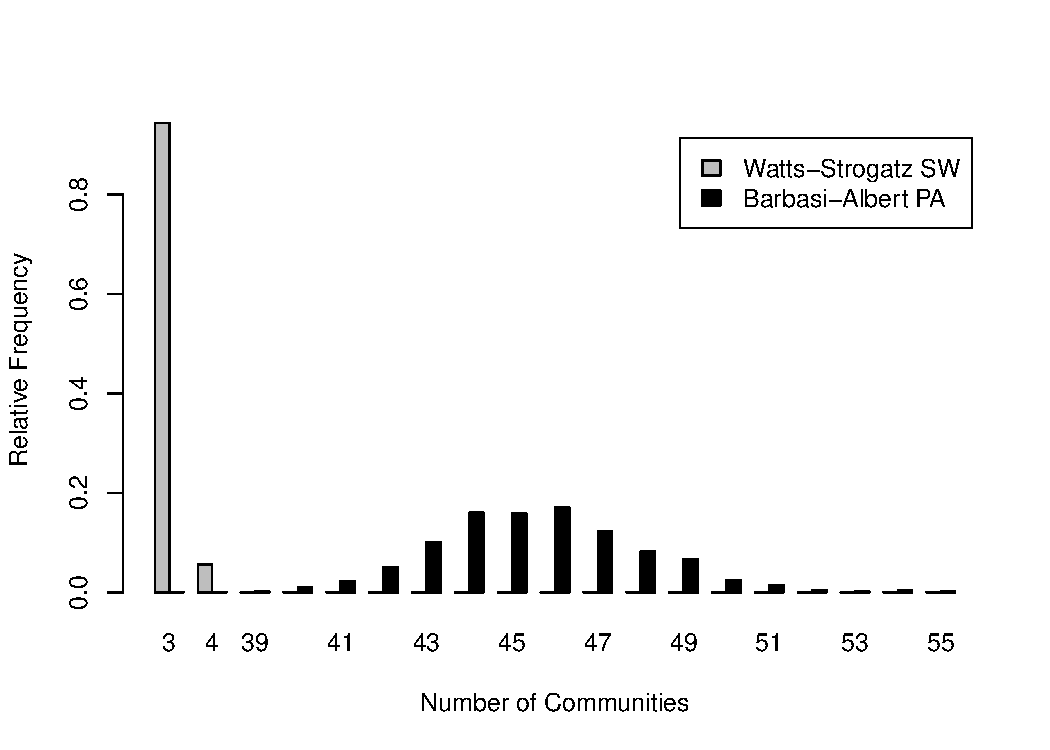
\includegraphics[scale=0.75]{Chapters/malaria/mechanisticComm}
\caption{Monte-Carlo simulations: Number of detected communities by the Watts-Strogatz and the Barab\'asi-Albert models}
\label{malaria_fig4}
\end{figure}

We also compared the clustering coefficient and the average shortest-path length. The observed clustering coefficient is 0.9645. Surprisingly, there is substantially more clustering in our malaria co-authorship network than expected from all 4 mathematical models (p-value < 0.0001). The expected clustering coefficient is 0.0596 (95\%CI: 0.05963068 -- 0.05964648) and 0.4334 (95\%CI: 0.4333912 -- 0.4334522) respectively for the classic random graph and the generalized random graph models.\\
Similarly, The Watts-Strogatz Small World model expected clustering is 0.7464 (95\%CI: 0.7464326 -- 0.7464356).\\
We observed an average shortest-path length of 2.99 in the malaria co-authorship network. This observed shortest-path length is significantly larger than what is expected from the random graph models (p-value < 0.0001) and significantly lower than what is expected from Watts-Strogatz small world model and the Barab\'asi-Albert preferential attachment model (p-value < 0.0001).\\The average shortest-path length is 1.94 (95\%CI: 1.941955 -- 1.941960) and 2.26 (95\%CI: 2.259468 2.259586) respectively for the classic random graph and the generalized random graph models.\\For the Watts-Strogatz small world and the Barab\'asi-Albert models, the average shortest-path length is respectively 3.83 (95\%CI: 3.81 -- 3.86) and 9.17 (95\%CI: 9.14 -- 9.21).\\~\\
All simulations were also performed on the giant component of the network and led to similar outcomes.%\\

\subsection{Statistical Modeling}
\subsubsection{Stochastic Block Model}
\label{sec:malaria_results_sbm}
The ICL plot on figure \ref{fig:malaria_sbmgof} shows that the malaria co-authorship network has been fit with 39 classes by the SBM with a degree of latitude of 30 to 39 classes being reasonable. The degree distribution of the fitted SBM (blue curve) provides a decent description of the observed distribution (yellow histogram). In the inter/intra class probabilities network, the vertices correspond to the 39 classes detected by the SBM. The vertex sizes are proportional to the number of authors assigned to each class. Each vertex is further broken down in a pie chart with each portion reflecting the relative proportion of the types of collaboration. Yellow represents the proportion of authors of international affiliations, orange represents regional authors who are affiliated with African institutions other than Beninese institutions, and green for authors affiliated to Beninese research institutions. In general, we observe a dominance of international and regional researchers over national researchers across all detected clusters.

\begin{figure}[!ht]
\centering
%\definecolor{shadecolor}{rgb}{0.969, 0.969, 0.969}\color{fgcolor}
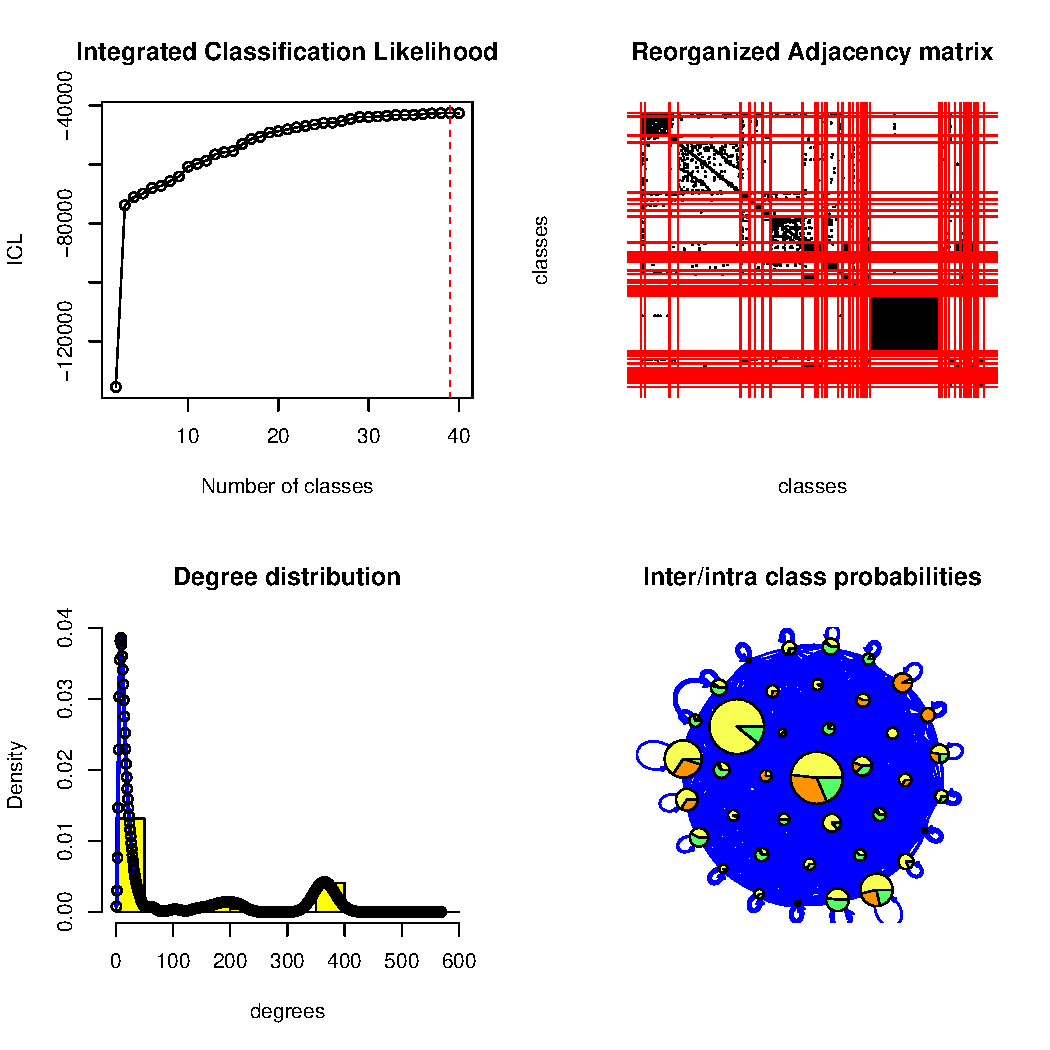
\includegraphics[scale=0.75]{Chapters/malaria/statMod/unnamed-chunk-1-1}
\caption{Summary of the goodness-of-fit of the SBM analysis on the Malaria co-authorship network.
%The SBM model was fit with 39 classes with a latitude of between 30 and 39 classes being reasonable.
}
\label{fig:malaria_sbmgof}
\end{figure}

A close look at the reorganized adjacency matrix, reveals the presence of 4 larger classes (classes number 2, 4, 10 and 27) and 35 other classes of smaller sizes. One of the larger class (class 27) displays a tendency of its members to only establish collaboration ties between themselves. This class seems to have the characteristics of a clique. Examination of the distribution of each class by their type of collaboration (Figure \ref{fig:malaria_dist}) indicates that this class of authors (class 27) is primarily made of international contributors to the malaria research effort in Benin. Although members of this class seem to have rare collaboration ties with members of other classes, we also notice the presence of very few broker authors as national liaisons between this class 27 and another larger class (class 2). Though, it also appears in the other three larger classes that the authors tend to primarily collaborate within their respective classes, they also tend to collaborate with authors of other classes.

\begin{figure}[!ht]
\centering
%\definecolor{shadecolor}{rgb}{0.969, 0.969, 0.969}\color{fgcolor}
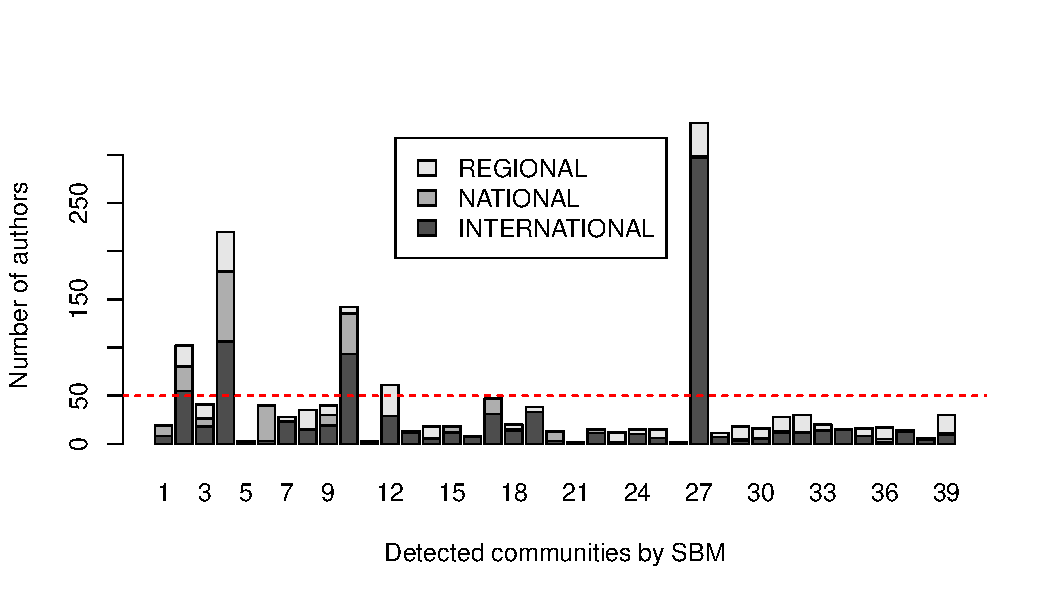
\includegraphics[scale=0.75]{Chapters/malaria/statMod/unnamed-chunk-2-1}
\caption{Distribution of national, international and regional authors by communities detected by the SBM in the Malaria network.}
\label{fig:malaria_dist}
\end{figure}

Figure \ref{fig:malaria_dist} also shows that the co-authorship malaria network in Benin is dominated by international researchers with national contributors unevenly distributed across the detected research communities. In order to better explain the inter/intra class interactions, we highlight in figure \ref{fig:malaria_sbmgof2}, the main classes driving the structure of the network. We present the results from the SBM on the classes with 50 authors or more. This reorganization clearly confirmed the presence of a clique of mainly international contributors who tend to collaborate rarily outside their class. The larger size here (Figure \ref{fig:malaria_sbmgof2}) is very diversed and contains all regional contributors to the malaria research effort. The presence of 3 smaller cliques which collaborate intensively between themselves is worth noting as well (See inter/intra class probabilities network on figure \ref{fig:malaria_sbmgof2}).

\begin{figure}[!ht]
%\definecolor{shadecolor}{rgb}{0.969, 0.969, 0.969}\color{fgcolor}
\centering
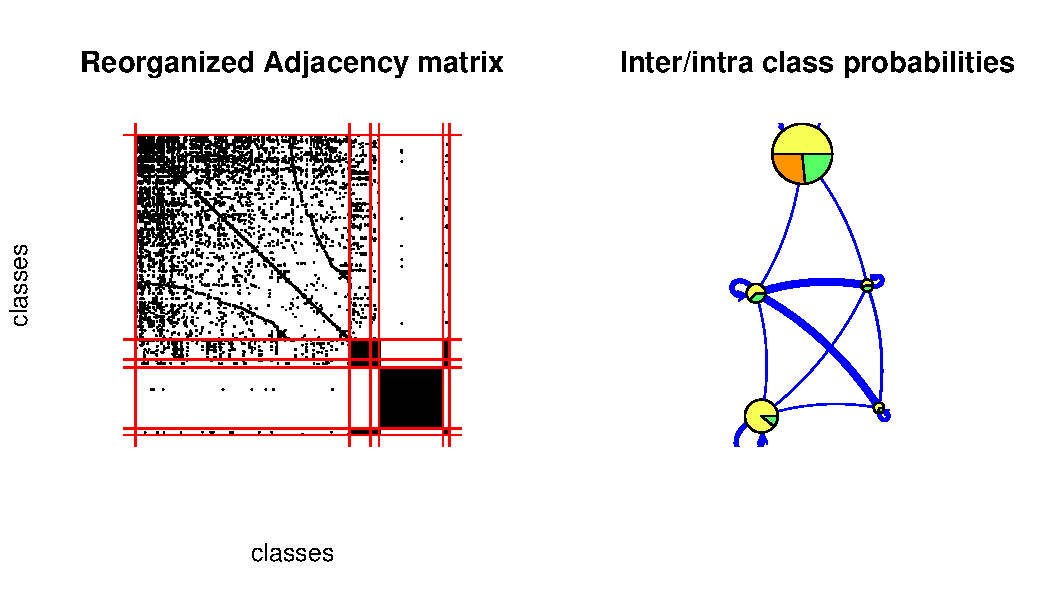
\includegraphics[scale=0.75]{Chapters/malaria/statMod/unnamed-chunk-3-1}
\caption{Summary of the goodness-of-fit of the SBM analysis highlighting interactions between the top 5 larger classes of the Malaria co-authorship network.}
\label{fig:malaria_sbmgof2}
\end{figure}
%
%\subsubsection{Dynamic Stochastic Block Model}
%%\label{sec:results_dynsbm}
%Figure \ref{fig:malaria_ICL} represents variation in ICL and log-likelihood by the number of detected research groups or communities by the dynSBM. The optimal number of groups determined by the ICL criterion is 14. However, the "elbow" heuristic suggests 5 detected groups. We therefore, ended up choosing the final dynSBM with 5 detected groups.
%
%\begin{figure}[!ht]
%%\definecolor{shadecolor}{rgb}{0.969, 0.969, 0.969}\color{fgcolor}
%\hspace{-1cm}
%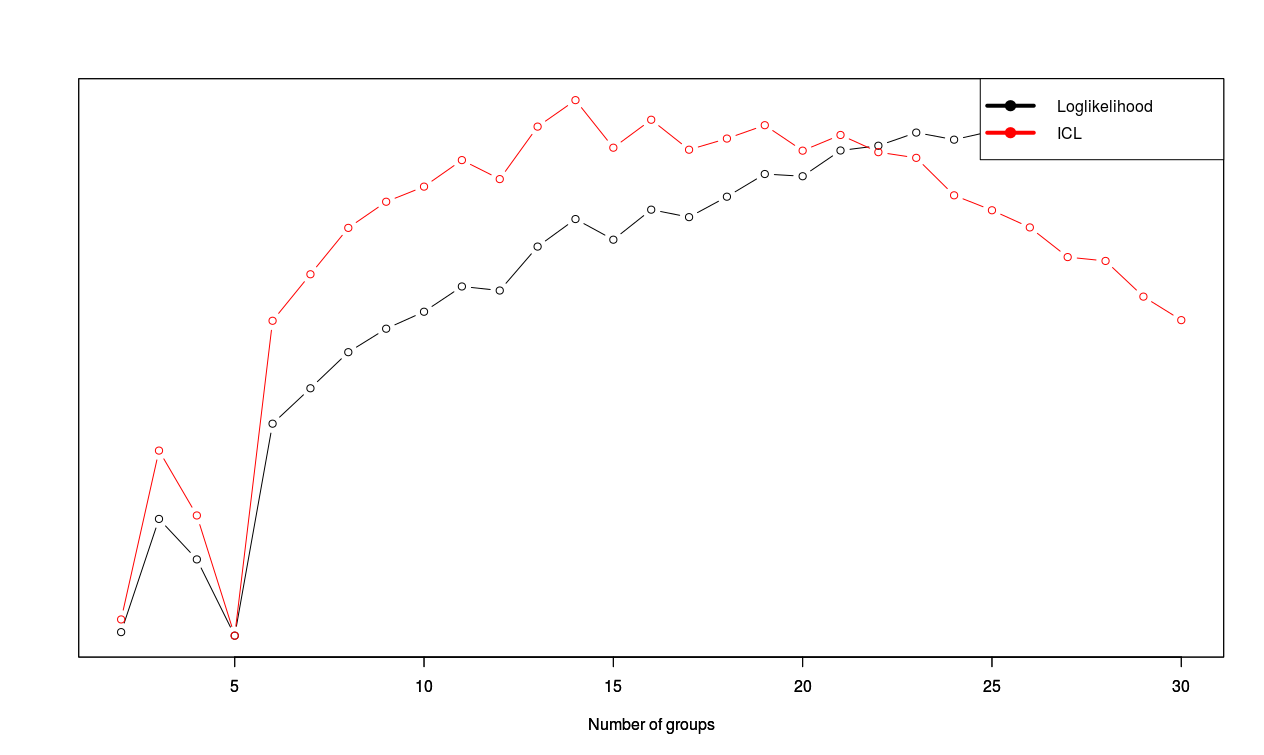
\includegraphics[scale=0.5]{Chapters/malaria/statMod/ICL_plot1}
%\caption{ICL and log-likelihood by number of detected research groups/communities.}
%\label{fig:malaria_ICL}
%\end{figure}
%
%Figure \ref{fig:malaria_connectivity} displays the structure of the dynamic network through the symmetric inter/intra group interaction properties. Interactions present in the figure are between nodes in any of the 5 detected groups to the others via a global $Q \times Q$ matrix. Each cell contains $T=7$ time points on the x-axis corresponding to the different time steps described in section \ref{sec:malaria_data}. As our network only contains binary edges, only interaction present is represented by the blue area. The $Q \times Q$ matrix shows directed interaction from group $q$ (rows) to group $l$ (columns). It is clear that intra-group interactions are more frequent across the study period, particularly in group 1, 3 and 5. For groups 1 and 5, this pattern appears stable in time while for group 3, it seems to have declined in the year 2014 followed by an upward trend in 015 and 2016. About inter-group collaboration ties establishment, the most striking pattern concerns authors in group 1 who tend to collaborate with authors in group 3. While this pattern seems unstable across the time steps, we note however an upward trend starting in 2014. Another important observation made here is the low inter-group interaction in group 2. Inter-group interaction in group 4 appears very unstable with some peaks in in 2007--2009 and in 2015.
%%We assess whether all authors have the same propensity to establish collaboration ties from one group to another one. Our observations suggest that globally, the average probability of between group collaboration ties establishment is estimated at 20\% across the 20 years of longitudinal network data.
%
%\begin{figure}[!ht]
%%\definecolor{shadecolor}{rgb}{0.969, 0.969, 0.969}\color{fgcolor}
%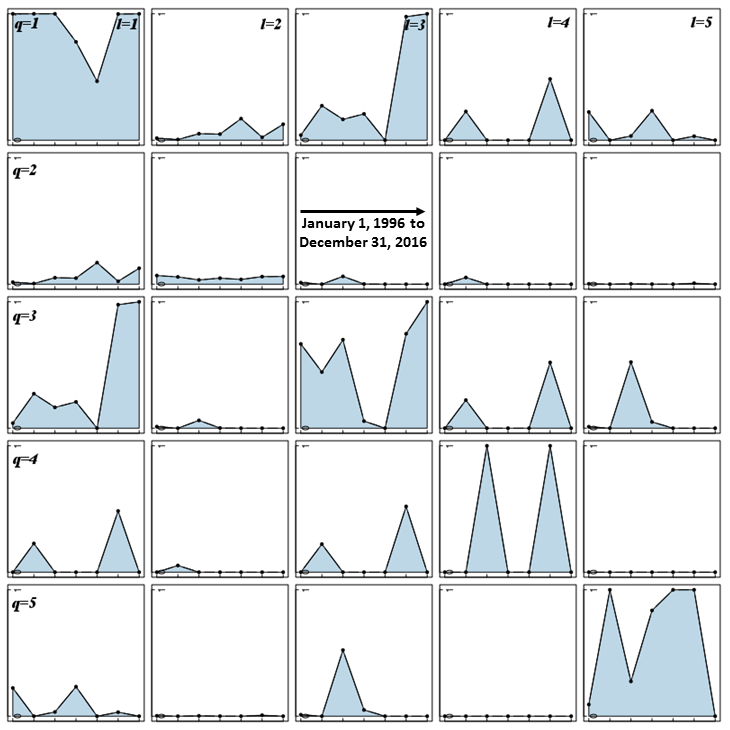
\includegraphics[scale=0.75]{Chapters/malaria/statMod/cPlot_q5}
%\caption{Interaction properties between research groups/communities in the Malaria co-authorship network.}
%\label{fig:malaria_connectivity}
%\end{figure}
\pagebreak
\subsubsection{Exponential Random Graph Model}
\label{sec:malaria_results_ergm}
Table \ref{tab:malaria_ergm} summarizes the results of the different models we fit to the observed network. Model 1 is analogous to the null model in a typical General Linear Model (GLM). The probability of any two authors establishing a collaboration tie is therefore expressed as the inverse logit of the edge coefficient. The inverse logit of a coefficient $x$ is defined as $logit^{-1}(x)=1/(1+exp(-x))$. The conditional log-odds for a collaboration between authors in the network is $-2.76$. The associated probability of any two authors establishing a collaboration tie is therefore $5.96\%$. To put this in perspective, this probabibility is the same as the density of the malaria co-authorship network. Since, our network is characterized by a high transitivity, we modeled the triangle ERGM term along with the edge term in model 2. We see some improvements in the model performance with a significantly positive but small triangle effect on the collaboration tie formation (Coefficient $= 0.08$, $p<0.001$). \\
In model 3, we describe the co-authorship network as a function of the number of collaborations, the number of publications, and the number of citations of authors inside the network. We also include confounding homophily term on cluster assignment from the SBM and on the collaboration type. Compared to models 1 and 2, model 3 has tremendously improved (See AIC and BIC in table \ref{tab:malaria_ergm}). The edge effect has decreased (Coefficient $=-7.98$, $p<0.001$) with the associated conditional probability (given all other terms in the model) equal to $0.03\%$. We observed a small, though positively significant effect of the number of collaborators and the number of publications on the odds of collaboration tie formation between any two authors. One unit increase in the number of collaborators increases the odds of collaboration tie by $2\%$ while one unit increase in the number of publications increases the odds of establishing a collaboration tie by $12.75\%$. On the other hand, model 3 has found a very small but significant negative effect of the number of times an author was cited on the odds of collaboration tie formation. One unit increase in the number of citation of a given author was associated with 1\% decrease in the odds of collaboration between two authors conditional on all the other terms in the model. \\
It clearly appears that the process underlying the malaria co-authorship network is driven by homophily on cluster assignment or membership to a specific research community and the type of collaboration. The conditional probability of two authors collaborating adjusted by the homophily on their membership to a research community is estimated at $8.32\%$ compared to the baseline probability of $0.03\%$ given all other terms in model 3. Adjusted by the collaboration type, the same probability is estimated at $0.05\%$ conditional on all other terms in the model. The overall conditional probability adjusting for all terms in model 3 is estimated at $14.06\%$ which is a lot greater than the $5.95\%$ estimated from model 1.\\
In model 4, we introduced  factor attributes on the collaboration type in order to investigate the likelihood of researchers affiliated to Beninese institutions to establish international and regional or African collaboration ties. While model 4 slightly improved upon model 3, it displays minor changes in the coefficient of the terms it has in common with model 3. Overall, compared to researchers with international research affiliations, researchers affiliated to Beninese research institutions have $37.7\%$ average decrease in the odds of establishing collaboration ties. On the other hand, researchers affiliated to other African research institutions have $78.6\%$ increase in the odds of establishing a collaboration tie than researchers affiliated to international research institutions. In other words, in model 4, the probability for researchers affiliated to international institutions to establish a collaboration tie is estimated at $14.19\%$, that of researchers affiliated to Beninese institutions is $10.72\%$, and that of researchers affiliated to African institutions other than Beninese institutions is $22.79\%$. \\
None of the structural models containing high order ERGM terms, nor the models containing the dyadic attribute terms converged after the maximum of 1,000 iterations making estimates from these models unreliable. This observation justifies the reason why we do not present the results from these models in table \ref{tab:malaria_ergm}. The unability of model containing structural terms to converge also makes it impossible for us to assess model degeneracy as recommended by Handcock et al. \cite{handcock_assessing_2003}.

\begin{table}[!h]
\caption{ERGM of the co-authorship Malaria network.} \scriptsize
\label{tab:malaria_ergm}
\hspace*{-1.5cm}
      \begin{tabular}{@{}lcclclclcl@{}}
        \toprule
           &  & Model 1 &  & Model 2  &  & Model 3&  & Model 4\\ \cmidrule{3-3} \cmidrule{5-5} \cmidrule{7-7} \cmidrule{9-9}
           &  & Estimate ($SE$) &  & Estimate ($SE$)  &  & Estimate ($SE$) &  & Estimate ($SE$)\\ \midrule
        Network structural predictor &  &   &  &  &  & &  & \\
        \hspace{10pt}Intercept(edge) &  & $-2.76\hspace{2pt}(0.00)^{***}$  &  & $-5.00\hspace{2pt}(0.01)^{***}$   &  & $-7.98\hspace{2pt}(0.02)^{***}$ &  & $-8.22\hspace{2pt}(0.02)^{***}$\\
        \hspace{10pt}Triangle &  & --   &  & $\hspace{6pt}0.08\hspace{2pt}(0.00)^{***}$   &  & --  &  & --\\ \\
        %\hspace{10pt}Degree &  & --   &  & --     &  & --  &  & --\\ \\
        Number of collaborations &  & --   &  & --  &  & $\hspace{6pt}0.02\hspace{2pt}(0.00)^{***}$  &  & $\hspace{6pt}0.01\hspace{2pt}(0.00)^{***}$\\% \\
        Number of publications &  & --   &  & --  &  & $\hspace{6pt}0.12\hspace{2pt}(0.00)^{***}$  &  & $\hspace{6pt}0.13\hspace{2pt}(0.00)^{***}$\\% \\
        Number of times cited &  & --   &  & --   &  & $-0.01\hspace{2pt}(0.00)^{***}$  &  & $-0.01\hspace{2pt}(0.00)^{***}$\\% \\
        Homophily on cluster assignment &  & --   &  & --    &  & $\hspace{6pt}5.58\hspace{2pt}(0.02)^{***}$  &  & $\hspace{6pt}5.68\hspace{2pt}(0.02)^{***}$\\% \\
        Homophily on collaboration type &  & --   &  & --    &  & $\hspace{6pt}0.46\hspace{2pt}(0.01)^{***}$  &  & $\hspace{6pt}0.61\hspace{2pt}(0.00)^{***}$\\ \\
        Factor attribute effect (collaboration type) &  &    &  &  &   &  &  & \\
        \hspace{10pt}International &  & --   &  & --   &  & --  &  & $REF$\\
        \hspace{10pt}National &  & --   &  & --   &  & --  &  & $-0.32\hspace{2pt}(0.02)^{***}$\\
        \hspace{10pt}Regional &  & --   &  & --   &  & --   &  & $\hspace{6pt}0.58\hspace{2pt}(0.01)^{***}$\\ \\ \midrule
        Number of iterations  &   & $6$   &  & $18$ &  & $8$  &  & $9$\\
        Akaike's Information Criterion (AIC)  &   & $725268$   &  & $660444$ &  & $220964$  &  & $217026$\\
        Bayesian Information Criterion (BIC)  &   & $725280$   &  & $660469$ &  & $221038$  &  & $217125$\\
        Model Log Likelihood  &   & $-362633$ ($df=1$)   &  & $-330220$ ($df=2$) &  & $-110475.9$ ($df=6$)  &  & $-108505.2$ ($df=8$)\\
        \bottomrule
      \end{tabular}
      \hspace*{-1cm}
      \raggedright \scriptsize
      $REF=$ reference, $SE=$ Standard Error, $df=$ degree of freedom\\
      ${ }^{***} p < .001$\\
      ${ }^{\hspace{3pt}**} p < .01$\\
      ${ }^{\hspace{5pt}*} p < .05$
\end{table}

Figure \ref{fig:malaria_ergm-gof} presents the goodness-of fit of model 4. The observed properties are depicted by the black lines. Gray lines with circles represent the 95\% confidence intervals for the simulated network properties. Goodness-of-fit is asserted when the black lines lie in-between the confidence intervals lines. The wide range of degree distribution of our co-authorship network makes it difficult to assess model fit in terms of degree distribution. But it is clear that in general, model 4 fits poorly to the observed network despite the highly significant estimates obtained. We therefore have strong evidence confirming that there is likely something other than the terms included in this model that are driving the structure of the network, possibly additional attributes our study did not control for. The following section attempts to address this shortcoming.

\begin{figure}[!h]
\centering
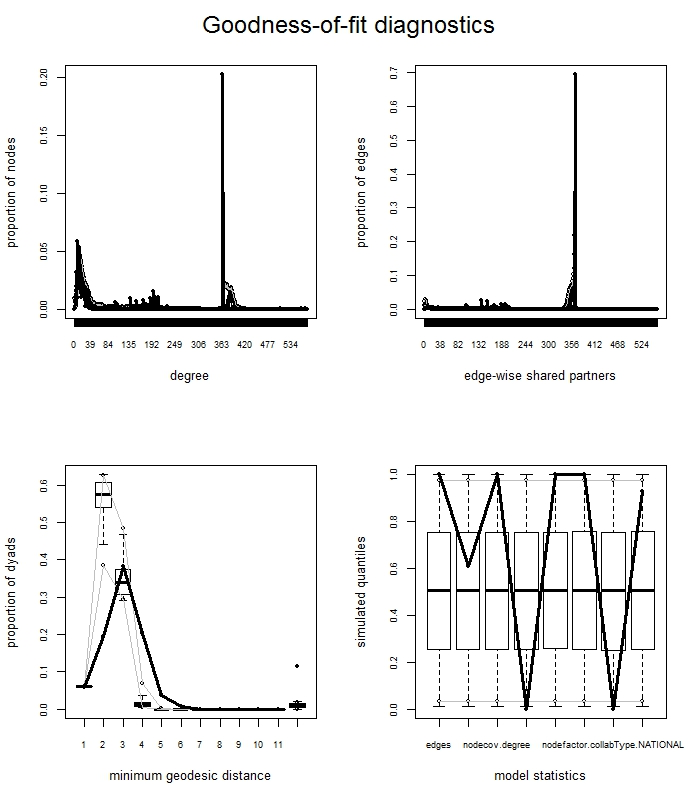
\includegraphics[scale=0.65]{Chapters/malaria/statMod/ergm_gof}
\caption{ERGM goodness-of-fit of final model 4 assessment.\\
%The observed properties are depicted by the black lines. Gray lines with circles represent the 95\% confidence intervals for the simulated network properties. Goodness-of-fit is asserted when the black lines lie in-between the confidence intervals lines.
}
\label{fig:malaria_ergm-gof}
\end{figure}

\pagebreak
\subsubsection{Temporal Exponential Random Graph Model}
\label{sec:malaria_results_tergm}
The observed cumulative network was subset in seven snapshots representing respectively the following time spans: 1996 -- 2006, 2007 -- 2009, 2010 -- 2011, 2012 -- 2013, 2014, 2015 and 2016. %\\
Figure \ref{fig:malaria_dynNetwork} displays the topological structure of the snapshots of the different time steps.

\begin{figure}[!ht]
\hspace{-1.25cm}
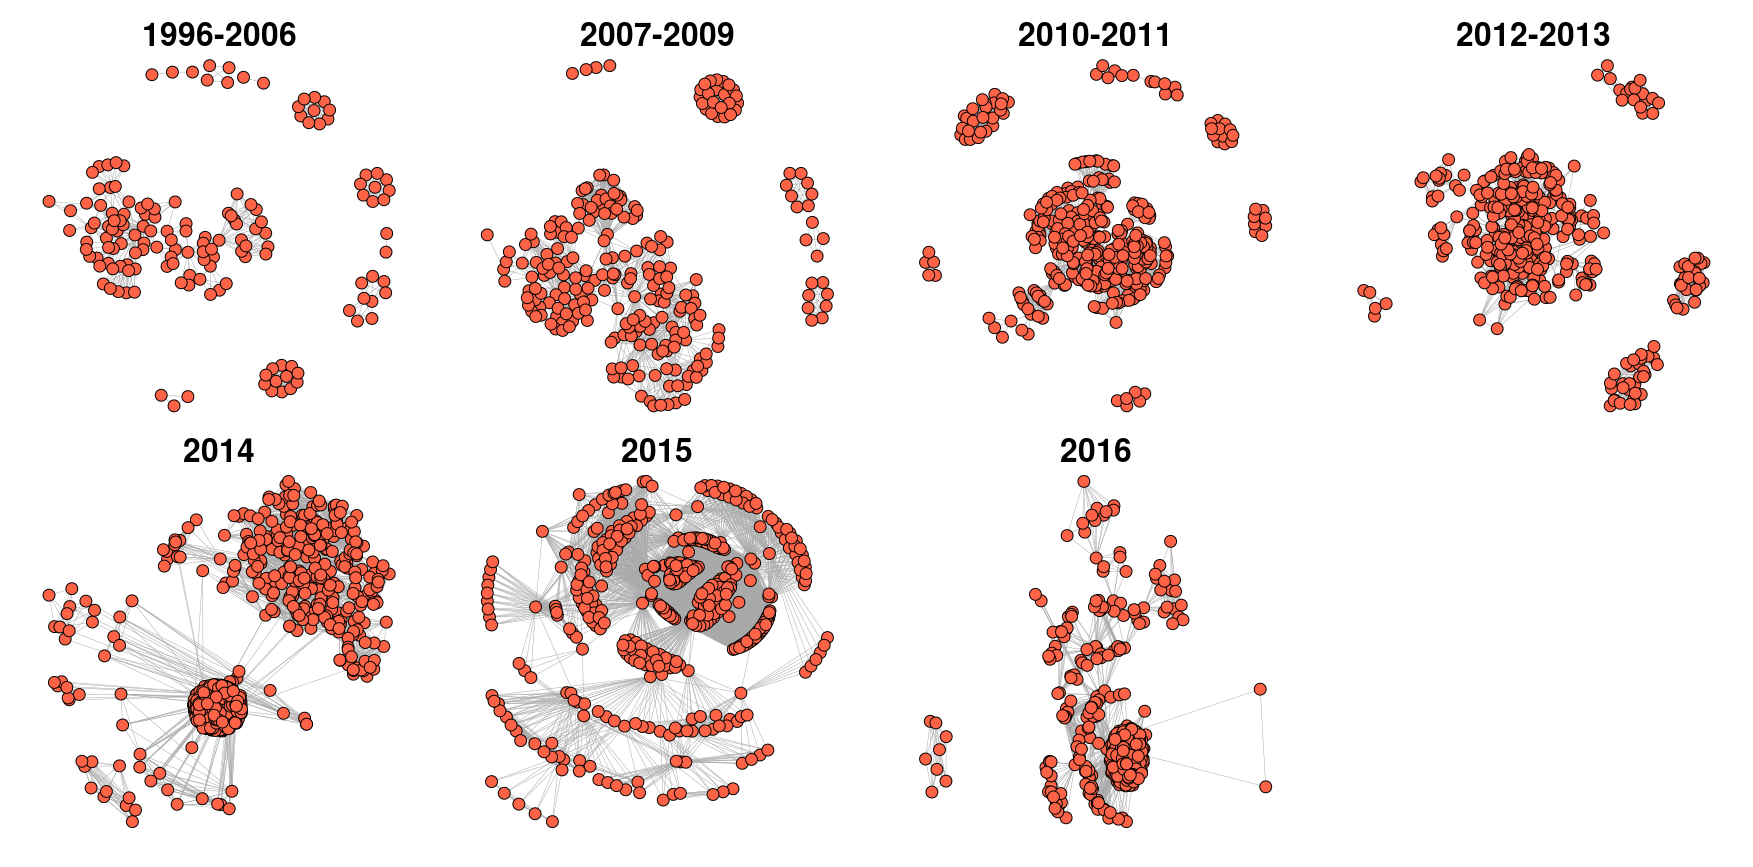
\includegraphics[scale=0.4]{Chapters/malaria/statMod/dynMNet2}
\caption{Topological structure of the different snapshots of the malaria co-authorship network.}
\label{fig:malaria_dynNetwork}
\end{figure}

Table \ref{tab:malaria_tergm} summarizes the results of the different temporal models we fit to the observed network. Models 1, 2, and 3 are equivalent to a pooled ERGM across the 7 different time points (Fig. \ref{fig:malaria_dynNetwork}). The null model of the TERGM (model 1) suggests that the baseline log-odds for collaboration tie formation between authors in the network is $-4.66$. This coefficient is equivalent to a baseline probability of $0.9\%$ for any two authors in the network to establish a stable collaboration tie. This probability is significantly lower than the 5.96\% baseline probability of collaboration tie establishment reported by the ERGM (section \ref{sec:malaria_results_ergm}). \\
Model 2 of the TERGM describes the co-authorship network as a function of the number of collaborations, the number of publications, and the number of citations of authors inside the network. It is also adjusted by homophily on cluster assignment from the SBM and on the collaboration type. Compared to model 1, model 2 has slightly improved (See AIC and BIC in table \ref{tab:malaria_tergm}). The edge effect has decreased (Coefficient $=-10.14$, $p<0.001$) with the associated conditional probability (given all other terms in the model) equal to $0.004\%$. We observed a relatively high positively significant effect of the homophily on cluster assignment on the odds of collaboration tie formation between any two authors. Adjusting for the other variables in model 2, authors of the same research groups/communities are $4.96$ times as likely to collaborate than authors that belong to different research groups. The effect of the other attributes in model 2 are minor. When we adjust for attribute effect on the collaboration type, we obtained model 3 which is slightly better than model 2. Relatively to model 2, the edge effect decreases more followed by an even stronger effect of the homophily on cluster assignment of the authors in the network (Coefficient $=5.06$, $p<0.001$). \\
After introducing temporal dependencies terms, we obtained model 4 which tremendously improved compared to models 1, 2 and 3. Model 4 confirms the observation made in section \ref{sec:malaria_results_ergm} that the process underlying the malaria co-authorship network is driven by homophily on cluster assignment or membership to a specific research community and the type of collaboration. It further confirms that the linear trend suspected observed in figure \ref{fig: malaria_pubDist} is significantly associated with the odds of collaboration tie formation in the Malaria co-authorship network. Model 4 suggests that the baseline conditional probability of any two authors to collaborate is estimated at 0.02\% given all other terms in the model. The coefficient associated to the dyadic stability term is 1.07 meaning that the odds of existent and non existent collaboration ties at one time point to remain the same at the next time point increased on average by $65.7\%$. In other words, the odds of new collaboration ties and non-ties to occur from one time point to another is $34.3\%$. In addition, the TERGM showed that the probability of sustainable collaboration tie formation among international researchers is $12.13\%$ versus $12.24\%$ for researchers affiliated with national institutions ($p>0.05$). However, this probability significantly increases to $20.26\%$ for researchers affiliated to African research institutions other than those in Benin. These probabilities confirm the results from the ERGM final model with respect to the higher probability of tie formation between researchers affiliated to African institutions other than Beninese institutions. None of the structural temporal models containing high order TERGM terms, nor the models containing the dyadic attribute terms converged after the maximum of 1,000 iterations making estimates from these models untrustful.\\

\begin{table}[!h]
\begin{center}
\caption{Temporal ERGM of Malaria co-authorship network.}
\label{tab:malaria_tergm}
\hspace*{-1cm}
\scriptsize
\begin{tabular}{@{}lcclclclcl@{}}
        \toprule
           &  & Model 1 &  & Model 2  &  & Model 3&  & Model 4\\ \cmidrule{3-3} \cmidrule{5-5} \cmidrule{7-7} \cmidrule{9-9}
           &  & Estimate ($SE$) &  & Estimate ($SE$)  &  & Estimate ($SE$) &  & Estimate ($SE$)\\ 
        \midrule
Network structural predictor & & & & & & & & \\
\hspace{10pt}Intercept(edge)   &  & $-4.66 \; (0.00)^{***}$ &  & $-10.14 \; (0.02)^{***}$ &  & $-10.45 \; (0.02)^{***}$ &  & $-8.65 \; (0.05)^{***}$ \\ \\
Number of collaborations          &  & --  &  & $\hspace{6pt}0.03 \; (0.00)^{***}$  &  & $\hspace{6pt}0.03 \; (0.00)^{***}$  &  & $\hspace{6pt}0.03 \; (0.00)^{***}$  \\
Number of times cited   &  & -- &  & $-0.03 \; (0.00)^{***}$ &  & $-0.02 \; (0.00)^{***}$ &  & $-0.03 \; (0.00)^{***}$ \\
Number of publications  &  & --  &  & $\hspace{6pt}0.45 \; (0.00)^{***}$  &  & $\hspace{6pt}0.46 \; (0.00)^{***}$  &  & $\hspace{6pt}0.45 \; (0.00)^{***}$  \\
Homophily on cluster assignment  &  & --  &  & $\hspace{6pt}4.96 \; (0.02)^{***}$  &  & $\hspace{6pt}5.06 \; (0.02)^{***}$  &  & $\hspace{6pt}4.79 \; (0.02)^{***}$  \\
Homophily on collaboration type   &  & --  &  & $\hspace{6pt}0.44 \; (0.01)^{***}$  &  & $\hspace{6pt}0.56 \; (0.01)^{***}$  &  & $\hspace{6pt}0.54 \; (0.01)^{***}$  \\ \\
Factor attribute effect (collaboration type) & & & & & & & & \\
\hspace{10pt}International & & -- & & -- & & $REF$ & & $REF$ \\
\hspace{10pt}National &  & -- &  & -- &  & $-0.10 \; (0.02)^{***}$        &  & $\hspace{6pt}0.01 \; (0.02)^{~~~~}$        \\
\hspace{10pt}Regional &  & -- &  & --  &  & $\hspace{6pt}0.55 \; (0.01)^{***}$  &  & $\hspace{6pt}0.60 \; (0.01)^{***}$  \\ \\
Temporal dependencies & & & & & & & & \\
\hspace{10pt}Dyadic stability          &  & --  &  & --  &  & --  &  & $\hspace{6pt}1.07 \; (0.01)^{***}$  \\
\hspace{10pt}Linear trends        &  & -- &  & -- &  & -- &  & $-0.18 \; (0.01)^{***}$ \\
%\hspace{10pt}Delayed reciprocity        &  &  -- &  & -- &  & -- &  & NA \\
\midrule
Akaike's Information Criterion (AIC)  &  & $\hspace{6pt}94681198$ &  & $\hspace{6pt}93740511$ &  & $\hspace{6pt}93737596$ &  & $\hspace{6pt}67005816$           \\
Bayesian Information Criterion (BIC)  &  & $\hspace{6pt}94681230$ &  & $\hspace{6pt}93740624$           &  & $\hspace{6pt}93737742$ &  & $\hspace{6pt}67005991$           \\
Model Log Likelihood &  & $-47340597$ &  & $-46870248$ &  & $-46868789$ &  & $-33502897$   \\
\bottomrule
%\multicolumn{5}{l}{\scriptsize{$^{***}p<0.001$, $^{**}p<0.01$, $^*p<0.05$}}
\end{tabular}
      \hspace*{-1cm}
      \raggedright \scriptsize
      $REF=$ reference, $SE=$ Standard Error\\
      ${ }^{***} p < .001$\\
      ${ }^{\hspace{3pt}**} p < .01$\\
      ${ }^{\hspace{5pt}*} p < .05$
\end{center}
\end{table}

Figure \ref{fig:malaria_tergm-gof} presents the goodness-of-fit assessment for the TERGM model 4. We can see that this model containing temporal dependencies fits better to the observed Malaria co-authorship network than the final ERGM model 4. While the first five subfigures compare the distribution of endogenous network statistics between the observed network and the simulated ones, the last subfigure presents the Receiver Operating Characteristics (ROC) and precision-recall (PR) curves. In general, the closer the curve is to the left-hand border and the top border of the ROC space, the more accurate the prediction is. On the other hand, the closer the curve is to the 45-degree diagonal of the ROC space, the less accurate is the prediction. The ROC for model 4 is depicted by the dark red curve compared to the ROC of a random graph depicted by the light red curve. Similarly, the dark blue curve represents the PR of model 4 versus the light blue curve representing the PR of a random graph \cite{leifeld_temporal_2015}. It clearly appears that the final TERGM model 4 outperformed the random null model with an Area Under the Curve (AUC) value estimated at $79.98\%$.

\begin{sidewaysfigure}
%\begin{figure}[!h]
\centering
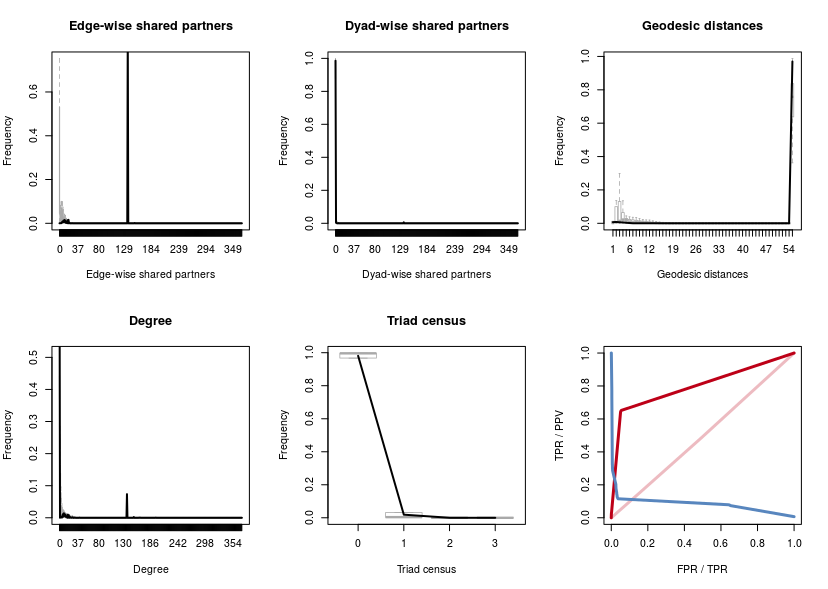
\includegraphics[scale=0.9]{Chapters/malaria/statMod/tergm_gof}
\caption{Goodness-of-fit assessment for the final Malaria TERGM Model 4 with temporal dependencies.}
\label{fig:malaria_tergm-gof}
%\end{figure}
\end{sidewaysfigure}
%~\\
\pagebreak
\subsubsection{Latent Network Model}
\label{malaria_sec:results_lnm}
Figure \ref{fig:malaria_lnm_viz} presents a 3-dimensional visualization of the Malaria co-authorship network, with layouts determined according to the inferred latent eigenvectors from the no pair-specific model (on top), the model containing nodal covariates (middle), and the model containing nodal and dyadic covariates (bottom). Blue vertices represent authors affiliated to Beninese research institutions, Red vertices are authors affiliated to international institutions, Gold vertices represent authors affiliated to African research institutions other than Benin, and White vertices represent authors with no determined affiliations. Node sizes are proportional to the betweenness value of each vertex. Looking at the three visualizations, it clearly appears that the first two visualizations are somewhat similar while the third is different. In fact, in the first two visualizations, the authors are clustered in mainly three clusters. We can see that all the authors affiliated to Beninese research institutions (in blue) are clustered in one cluster while authors with international affiliations (in red) and regional authors (in gold) are distributed across all three main clusters. These observations suggest a significant geography effect on the odds of collaboration tie establishment in the malaria co-authorship network. \\The first two visualizations also highlight key brokers that liaison between clusters. 
%%%Added from suggested corrections
%%From the WOS API, those key brokers also appears to be the authors with the highest citation count. For example, in the first two visualizations on figure \ref{fig:malaria_lnm_viz}, the brokers with affiliations to national institutions are MASSOUGBODJI ACHILLE, AKOGBETO MARTIN, and SANNI AMBALIOU. These authors are also the ones with the highest citation counts. Such an observation is not surprising given their long tenure, their publication records, and known expertise in malariology.
%%%
In the third visualization, on the other hand, there appears to be only one main cluster. This last observation suggests that the nodal covariates and mainly homophily on research community membership and type of affiliation explain much less coarse-scale network compared to dyadic covariates. Indeed, when the dyadic covariates are added to the model, there is less structure left to be captured by the latent variables. These results compensate the lack of-fit of the ERGM model and confirmed our findings in the previous section.

\begin{figure}[!h]
\center
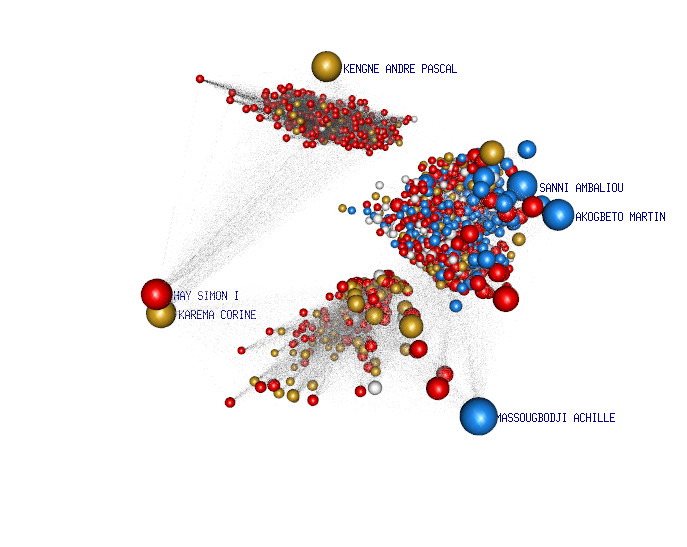
\includegraphics[scale=0.3,trim={5cm 0 0 0}]{Chapters/malaria/statMod/lnm_mod1_null.png}
\vspace{0px}\\
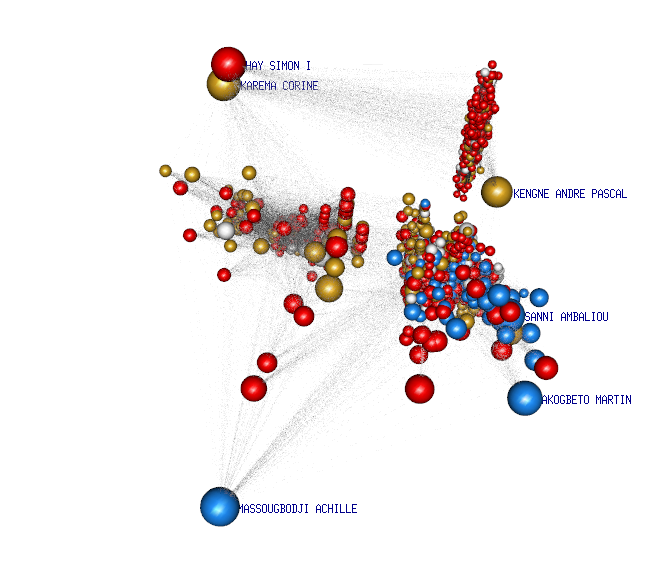
\includegraphics[scale=0.3,trim={5cm 0 0 0}]{Chapters/malaria/statMod/lnm_mod5_nodes.png}
\vspace{2px}\\
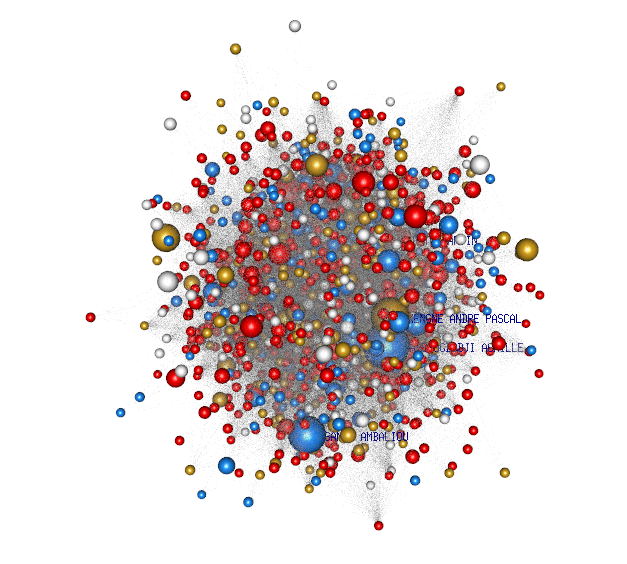
\includegraphics[scale=0.3]{Chapters/malaria/statMod/lnm_mod6_all.png}
\caption{Visualizations of the Malaria co-authorship network with layouts determined according to the inferred latent eigenvectors in the LNM models (International (Red); Regional (Gold); Local (Blue)).
% with no pair-specific covariates (top), nodal covariates (middle), and all covariates (bottom).
}
\label{fig:malaria_lnm_viz}
\end{figure}

The ROC curves on figure \ref{fig:malaria_lnm_roc} show that the first two models appear to be comparable in their performance from the perspective of edge status prediction with an Area Under the Curve (AUC) being roughly 98.8\%. %The third model, with added dyadic covariates, has a perfect fit to the observed network data.

\begin{figure}[!h]
\centering
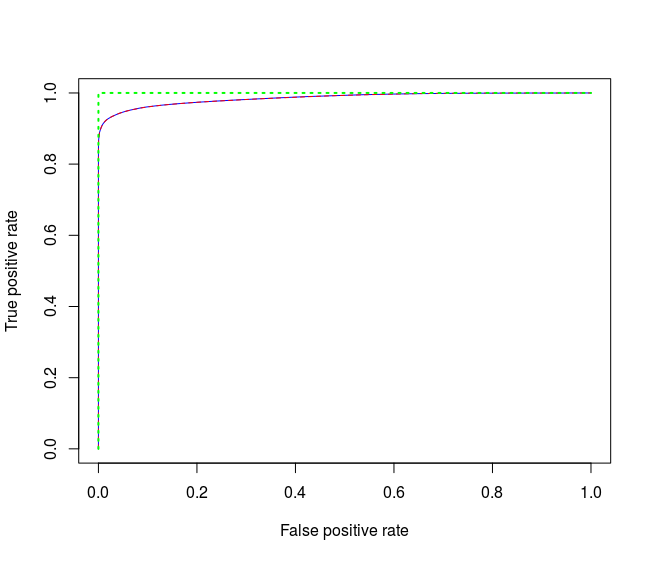
\includegraphics[scale=0.75]{Chapters/malaria/statMod/lnm_ROC.png}
\caption{ROC curves comparing the goodness-of fit of the Malaria co-authorship network for three different eigenmodels, specifying (i) no pair specific covariates (blue), (ii) nodal covariates (red), and (iii) nodal and dyadic covariates (green), respectively.}
\label{fig:malaria_lnm_roc}
\end{figure}
~\\
\pagebreak
\section{Discussion and Conclusion}
\label{sec:malaria_discussion}
In this chapter, we provide insights in the structural characteristics of the malaria co-authorship network in the Republic of Benin over a relatively long period. The 20 years of data collected coincides with the onset of active malaria research from 1996 until today. The significant increase in malaria research and collaborations (figure \ref{fig:malaria_dist}) between the authors over the years is an expected finding given the regain and renewed interest in malaria control and elimination goals set forth \cite{alonso_research_2011, breman_eradicating_2009}. Our results show that the mechanism underlying the formation of the malaria co-authorship network in Benin is not random. It further demonstrates that the malaria research collaboration network in Benin is a complex network that seems to display small-world properties (often referred to as "six degrees of separation"). \\%~\\
The non-trivial number of authors with higher order of magnitudes confirms the presence of closed research groups where collaborative research likely happens only among members. In other words, interdisciplinary collaboration tends to occur at higher levels between prolific researchers with the majority of the collaborations happening between researchers from the same scientific communities. Prominent authors with long tenure tend to collaborate with similar authors, young or less prolific authors tend to collaborate with both prolific authors and authors with very few collaborations. Similar findings were reported by Janet Okamoto \cite{the_centers_for_population_health_and_health_disparities_evaluation_working_group_scientific_2015} who studied scientific collaboration on a much smaller scale. %\\
Key brokers facilitate scientific collaborations within and outside their scientific community \cite{bellanca_measuring_2009}. Betweenness centrality measures identify such brokers who are important hubs for inter and transdisciplinary research. Many of the main brokers proved to also be the most connected and the most central authors confirming the presence of long publishing tenure authors in our network \cite{li_co-authorship_2013}. %\\
The flow of information in this network in Benin is slow as it only relies on 16 authors representing less than 1\% of all the authors in the network. Such a low information flow was also reported by Salamatia and Soheili \cite{salamati_social_2016} in a 2016 study on a co-authorship analysis of Iranian researchers in the field of violence. Generally, the most important authors in a co-authorship network are the ones with the highest degree of collaborations \cite{bales_social_2008, bales_evolution_2011}. However, to the long-term substainability of the malaria research network in Benin, the 16 authors identified as cut vertices are the most important authors. In other words, the removal of less than 1\% of the authors from the network would lead to its collapse. Such a collapse would undoubtedly be detrimental to the future of malaria research in Benin. This finding clearly confirms the conclusion of Toivanen and Ponomariov \cite{toivanen_african_2011} that the African research collaboration network is vulnerable to structural weaknesses and uneven integration.\\%~\\
Small-world networks are known to have small shortest path distance and a high clustering coefficient. Although this co-authorship network seems to display such properties, the Monte-Carlo simulations revealed that the observed network has unexpected properties compared to classic small-world networks. A study of co-authorship network conducted on Chagas disease has found similar findings \cite{gonzalez-alcaide_scientific_2012}. Unlike our study, the authors of the Chagas disease co-authorship study did not deepen their analysis to confirm the small-world nature of their observed network. Other mechanisms such as preferential attachment have been found to explain the structure of international scientific collaboration network \cite{wagner_network_2005}. Unlike those studies, our network displayed unexpected properties that are more extreme than the 4 mathematical models we simulated. Our network has significantly higher clustering than expected from the 4 mathematical models presented here. One observation we are sure of is that none of the random graph models used here tend to explain the growth and the structure of the malaria co-authorship network in Benin. We therefore claim without any doubt that the structure and growth of our network is not random confirming the presence of hidden factors explaining the current structure of the network. Assessing such factors and the extent to which they influence scientific collaborations is important for the future of malaria research and its long-term sustainability. Unfortunately, none of the proposed mathematical models seem to accurately describe the observed structure of the network. To address these limitations, advanced statistical modeling was used to further explain the structure of the network. \\%~\\
Our first approach to modeling our network relied on the use of SBM. In addition of being a model based clustering method, the SBM identified important organizational and interactional patterns in the network. It identified a large clique of mainly international researchers with little or no collaborations with other research groups.
%%%Added from suggested corrections
It also identified the main broker authors in the network. For example, in the first two visualizations on figure \ref{fig:malaria_lnm_viz}, the brokers with affiliations to national institutions are MASSOUGBODJI ACHILLE, AKOGBETO MARTIN, and SANNI AMBALIOU. These authors are also the ones with the highest citation counts. Such an observation is not surprising given their long tenure, their publication records, and known expertise in malariology, parasitology and medical entomology. 
%%%
The overwelming dominance of regional and international players in the network is consistent with previous observations by Onyancha and Maluleka \cite{onyancha_knowledge_2011} who concluded on a much higher likelihood of Sub-Saharan African countries to collaborate with non-African states. \\
Overall, the ERGM and TERGM show that the mechanistic phenomenon driving collaboration ties in the malaria research in Benin is influenced by homophily on the type of affiliation (national, international or regional) and on membership to a research group or cluster, verifying therefore our third hypothesis. The models clearly show that the dominance of the Beninese malaria research arena by international and regional players, and further demonstrates the lower likelihood of local Beninese researchers to establish international collaboration ties compared to regional researchers. This latter finding has been confirmed by the LNM which also confirms our second hypothesis. The ERGM and the TERGM revealed that factors such as number of publications, number of citations and number of collaborations are associated to higher likelihood to establishing collaboration ties, confirming therefore our first hypothesis. \\
It is worth noting that many of the studies on co-authorship network analysis are descriptive in nature. This study is one of the rare co-authorship network analysis to model a co-authorship network using advanced statistical models. ERGM is the leading approach to modeling network \cite{schmid_exponential_2017}. The literature has reported application of this model in studying various social network such as the analysis of friendship and obesity \cite{valente_adolescent_2009,de_la_haye_obesity-related_2010}, the exploration of the association between hormone and social network structure \cite{kornienko_hormones_2014}. Similarly to friendship networks, the use of ERGM to model co-authorship networks is easily justified. However, the size of our network prevented the fitting of complex models including dyadic and structural terms. In addition, our best ERGM model failed to adequately fit the observed network data. This lack of goodness-of fit, according to Hunter, Goudreau and Handcock \cite{hunter_goodness_2008}, could be improved by including the geometrically weighted edgewise shared partner, geometrically weighted dyadic shared partner, and geometrically weighted degree network statistics to our model. Although, we follow such recommendations by including these structural network statistics to our final model, the ERGM model failed to converge after a maximum of 1,000 iterations. At about 750 iterations, we noticed that the processing became both computationally intensive and expensive in terms of CPU time and memory usage. In a recently published paper, Schmid and Desmarais \cite{schmid_exponential_2017} acknowledged the difficulty of fitting network which size is of the order 1,000 vertices using ERGM. They recommended that using the maximum pseudolikelihood estimation (MPLE) instead of the Monte Carlo maximum likelihood (MCMLE) could tremendously reduce computation time. Having followed these recommendations too, the ERGM model containing dyadic and structural terms still failed to converge. By finally including temporal dependencies and fitting a temporal ERGM, we have tremendously improved the fitness with a predictive performance of roughly 80\%. Nevertheless, we suspect that the number of edges, the large size of the network added to the possibility of hidden/latent variables might justify the failure of the models containing the dyadic and structural endogenous terms to converge. We remedy this situation by applying LNM to the observed network data. \\
All three latent network models (LNM) proved to be successful in fitting the observed network data. 
%The fact that the third latent network model include all nodal and dyadic variables could explain its perfect fit. In addition, there was less structure left to be captured by the latent variables in this model. On the other hand, the first two latent network models gave us confident in validating the results of the TERGM. \\
A study by Kronegger et al. \cite{kronegger_collaboration_2012} conducted an investigation aiming at describing the collaboration in Slovenian scientific communities using data from four different disciplines. Their methodological approach is consistent with ours. The main difference is their application of Stochastic Actor-Oriented Model (SAOM) on the dynamics of their co-authorship networks. Since the SAOM is an actor-oriented modeling method and we are interesting in tie prediction here, we relied rather on a tie-oriented approach by applying the TERGM to our network data. \\
Our results suggest that the regain in Malaria research funding has appealed to research groups all around the world, hence the explosion in publications number and research collaborations. 
As the disease continues to be main public health concern in the Republic of Benin, it is essential to consolidate the knowledge generated from the numerous studies on the disease and reinforce the different  communities involved in the research effort. In addition, there is an urgent need to reinforce the malaria research network in Benin by continuously supporting, stabilizing the identified key brokers and most productive authors, and promoting the junior scientists in the field. However, we observed a tendency of the international researchers to only collaborate among themselves. Although the rise in scientific collaboration between advanced and developing nations \cite{wagner_science_2001}, the latter observation may limit effective and sustainable technology transfer in Benin. It is possible that some of the isolated cliques within the network have top-notch research capabilities and skills researchers affiliated to Beninese institutions can acquire, should the research groups be more inclusive. Unfortunately, our visualizations showed that broker authors that liaison those closed groups to national researchers tend to be regional or international researchers as well. We therefore recommend, that policies should be designed, at international, regional and country level, to diversify research groups operating in any Sub-Saharan African countries. Such policies will ultimately enable effective technology transfer, multidisciplinarity, and promote junior African researchers to advance the search of a solution to the Malaria problem in Africa and particularly, in Benin.


%%%%%%%%%%%%%%THIS SECTION IN GENERAL CONCLUSION
%Since co-authorship networks are dynamic in nature, the application of temporal or dynamic modeling techniques is the major strength of our research. Other strengths include its application of not only descriptive methods but also robust network analysis methods such as inferential methods like Monte-Carlo simulations, unlike most studies on co-authorship analysis. Our data mining strategy involved a robust machine learning algorithm that helped address the crucial issue of the disambiguation of authors names and assign a unique identification to each of them. This technique maintained a good quality of the data collected throughout the pre-processing and analysis steps. To the best of our knowledge, our study is the first to describe the malaria research collaborations network via co-authorship network analysis in Benin. It is also the first to apply statistical network models to investigate co-authorship network in a specific research area in an African country.\\%~\\
%The fact that our study collected data only from the Web Of Science can be considered as an important limitation of this study. However, according to Falagas and colleagues \cite{falagas_comparison_2007}, who compared PubMed, Scopus, Web Of Science and Google Scholar in their paper, the Web Of Science appears as a reasonable scientific database source for our analysis. In addition, it proved to cover a wide range of both old and recently published papers. Falagas and colleagues \cite{falagas_comparison_2007} found PubMed to be the optimal choice in terms of scientific database. For that reason we did run the same bibliographic search in PubMed. Unfortunately, the Web Of Science returns more relevant data than PubMed. Another limitation worth noting is that this study only looks at a snapshot of the malaria research network on a static fashion. There is also a need to apply dynamic statistical models such as Temporal Exponential Random Graph \cite{leifeld_temporal_2015} and Dynamic Stochastic Block \cite{matias_statistical_2016} modeling to better understand the temporal dynamic of collaboration formation in this network. Yet another limitation is inherent to the nature of all co-authorship studies. Collaborators, in a co-authorship network, do not often come from the same scientific discipline, or do not play the same roles on a particular research project. The data we collected did not allow us to accurately assess or even infer the disciplines each author came from or their specific contribution in the published document.\\%~\\
 % HIV/AIDS Co-authorship Network

%*******10********20********30********40********50********60********70********80

% For all chapters, use the newdefined chap{} instead of chapter{}
% This will make the text at the top-left of the page be the same as the chapter

\chap{Results: The Tuberculosis Co-authorship Network}

%\section{Background}
%Tuberculosis (TB) is a highly contagious and airborne infectious disease that is caused by \textit{Mycobacterium tuberculosis}. In 2015, TB was one of the top 10 causes of mortality worldwide. The global burden of TB worldwide is estimated at more than 1.8 million deaths including 0.4 million deaths among people living with HIV/AIDS in 2015. The disease has reportedly caused more deaths that same year than malaria and HIV/AIDS combined \cite{world_health_organization_global_2016}. \\
%At the Millenium Challenge summit of 2000, the Millenium Development Goal 6 (MDG6) was declared and aimed at a drastic reduction of the transmission of HIV/AIDS, Malaria and other diseases such as TB \cite{world_health_organization_mdg_2013}. According to the World Health Organization, the "World is on track" to achieving the MDG6 despite complicating factors such as the coinfection TB/HIV and the multidrug resistance in \textit{Mycobacterium Tuberculosis} \cite{world_health_organization_global_2016,falzon_world_2017,lynch_multidrug-resistant_2013}. 
%Despite those limitations, it is worth noting that the significant efforts made in terms of the increase in the global funding disturbement for TB \cite{global_fund_making_2011} has contributed to significantly scaling research efforts at reducing TB related mortality and morbidity. In the Republic of Benin where TB is the third major public health concern behind Malaria and HIV/AIDS, the increase in TB funding has led to a decrease of 0.8\% and 1.2\% respectively of the incidence and the annual death rate of TB in 2010 \cite{world_health_organization_global_2010}.\\ %For example, the year 2010 recorded the highest peak in the Global Fund disbursement for TB with an estimated 416 millions US dollars in 2010 \cite{global_fund_making_2011}.
%Achieving the MDG6 has resulted in change in public health policies accompanied by an increase in scientific research on Malaria, HIV/AIDS and TB \cite{world_health_organization_global_2010}. Scientific collaborations give researchers the opportunity to work and learn from each other. Such collaborations are further needed to overcome the overgrowing challenge of co-infections between HIV/AIDS and Tuberculosis \cite{corbett_growing_2003,gandhi_hiv_2010}. Identifying the main authors driving the publication efforts on TB and their collaborative patterns is an important basis for future public health strategies and to cooperative and translational scientific research initiatives \cite{gonzalez-alcaide_scientific_2012}. One approach to such an endeavour is the Social Network Analysis (SNA) of collaboration networks through co-authorship networks \cite{scott_social_2017,uddin_trend_2012}. \\
%The paradigm of co-authorship network is rooted in network theory, with the set of nodes represented by the authors and the set of edges describing the relationship between them \cite{newman_structure_2001}. The analyses of how complex TB co-authorship networks form and evolve in time is crucial for identifying leading researchers in the field, and describe their extant to collaborate with their peers as well as the impact of their research \cite{gonzalez-alcaide_coauthorship_2008}. An example of such investigation is illustrated in Newman scientific collaboration paper series on Biomedical research, physics and computer science co-authorship network \cite{newman_structure_2001,newman_scientific_2001-1,newman_scientific_2001,newman_coauthorship_2004}.\\
%The objective of this study was to analyze the authorship of scientific manuscripts on Tuberculosis in the Republic of Benin published in scientific journals indexed in the Web Of Science (WOS) from January 1, 1996 to December 31, 2016. By describing the structure of the TB network in Benin, we aim at providing a basis for research prioritization \cite{ghafouri_social_2014}, identification of prolific researchers, better design, strategic planning and effective implementation of research programs \cite{morel_co-authorship_2009}. 

\section{Data}
\label{sec:tb_data}
The literature search was conducted in the Web Of Science using combinations of TB related MeSH terms including "Tuberculosis", "Mycobacterium", "Infection". We restricted the search to the period from 1996 to 2016 and to "Benin" for country. We further screened the papers in order to only select those published by Beninese authors, or papers published on TB from Benin. All published documents under considerations included at least one Author from Benin. No restriction was placed upon the document types. We first started querying with each term independently, we then combined the other terms so the query return the maximum number of results. The  Full citations information containing the authors' names, their institutional affiliations, the year of publication, as well as the number of times the document was cited were recorded as a bibliographic corpus in text format. After a second screening only research that have met the above listed inclusion criteria and that were published between January 1, 1996 and December 31, 2016 were selected. \\
The final query set (Table \ref{table: tb_search}) returned returned 109 records. After a rigorous screening process carried out by all the authors, 37 documents met the selection criteria. On average, there was 9.38 authors per published document. \\

\begin{table}[h!]
\caption{TB Bibliographic Search Queries.}
\label{table: tb_search}
\centering \small
%\hspace{0.25}
\begin{tabular}{llc}
\toprule
Set & \multicolumn{1}{c}{Queries} & Results \\
\midrule
\#1 & TOPIC: (Tuberculosis) AND ADDRESS: (BENIN)  & 109 \\\\
\#2 & \begin{tabular}[c]{@{}l@{}}TOPIC: (Tuberculosis),\\Refined by: COUNTRIES/TERRITORIES: (BENIN )\end{tabular} & 77 \\\\
\#3 & \begin{tabular}[c]{@{}l@{}}TOPIC: (Mycobacterium Tuberculosis),\\AND ADDRESS: (Benin)\end{tabular} & 77 \\\\
\#4 & \begin{tabular}[c]{@{}l@{}}TOPIC: (Tuberculosis) OR TOPIC: (Infection) AND ADDRESS: (BENIN),\\Refined by: COUNTRIES/TERRITORIES: (BENIN)\end{tabular} & 89 \\
\midrule
Final Set & \#1 OR \#2 OR \#3 OR \#4 & 109\\
\bottomrule
\end{tabular}
\end{table}

After the Author Name Disambiguation, we identified 173 unique authors with a precision of 99.99\% and a recall of 99.99\%. The generated multigraph co-authorship network therefore contained 173 vertices (authors) and 1,937 parallel edges (collaborations). As displayed in figure \ref{tb_pubDist}, we can see the significant increase in publications, scientific collaborations and the number of authors involved in TB research from 2008 until 2016. This general upward trend seems to be linear from the year 2008 to 2016. \\

\begin{figure}[h!]
\centering
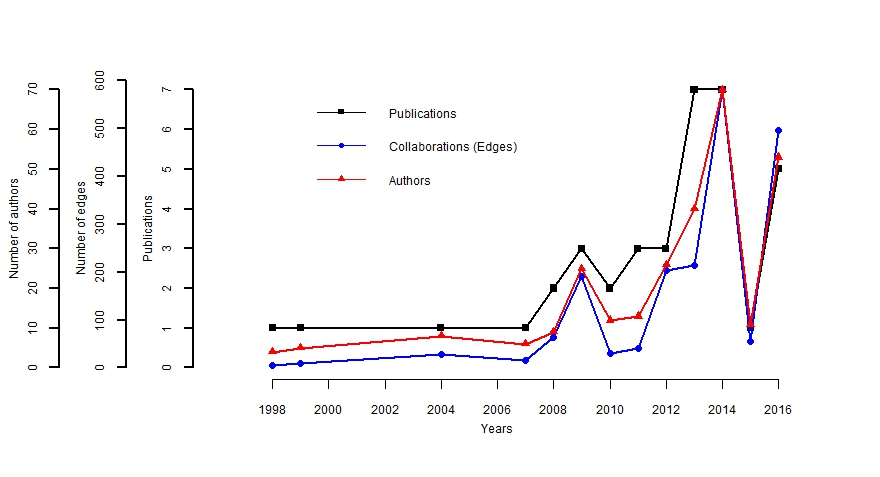
\includegraphics[scale=0.6]{Chapters/tb/pubDist}
\caption{Evolution of the published TB related documents, authors and collaborations from January 1996 to December 2016}
\label{tb_pubDist}
\end{figure}

\section{Descriptive Data Analysis}
\label{sec:tb_descstat}
For the multigraph network, the degree distribution ranged between 2 and 165 with an average degree distribution of 17.36 and a median of 15. In addition, there was a substantial number of vertices with low degrees (Fig. \ref{tb_fig1}). The log scale distribution of the degrees on figure \ref{tb_fig2} reveals that there was a tendency of prolific authors to collaborate with less prolific authors. 

\begin{figure}[h!]
\centering
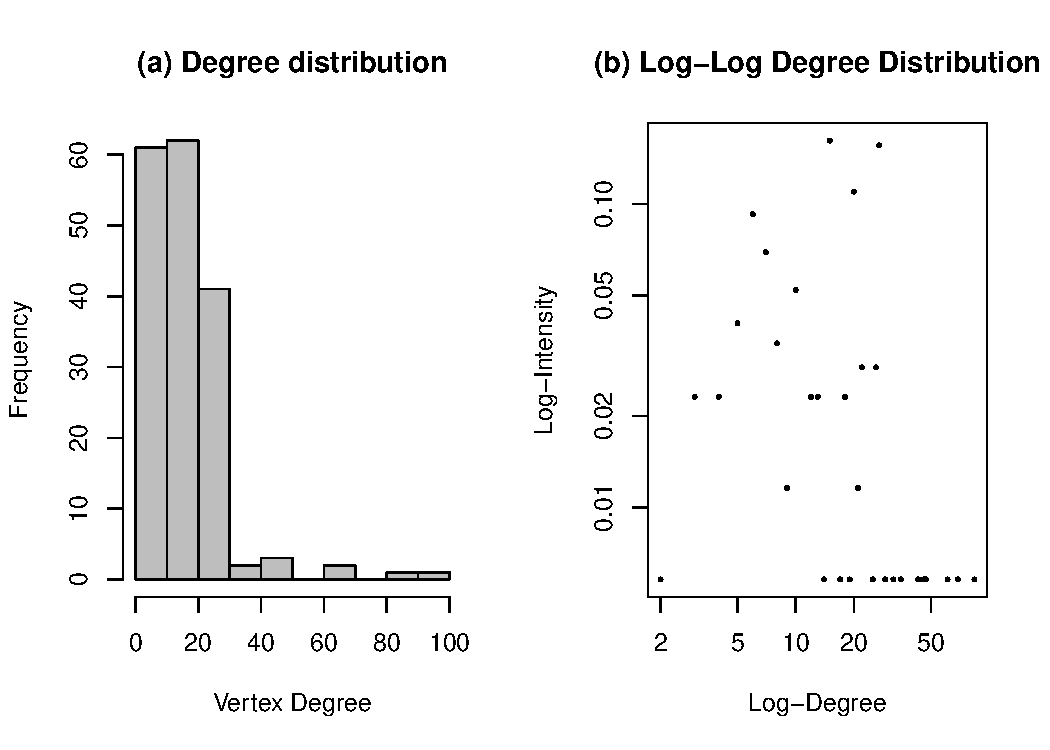
\includegraphics[scale=0.65]{Chapters/tb/degreeDistribution}
\caption{Degree distribution of the TB Co-authorship network}
\label{tb_fig1}
\end{figure}

\begin{figure}[h!]
\centering
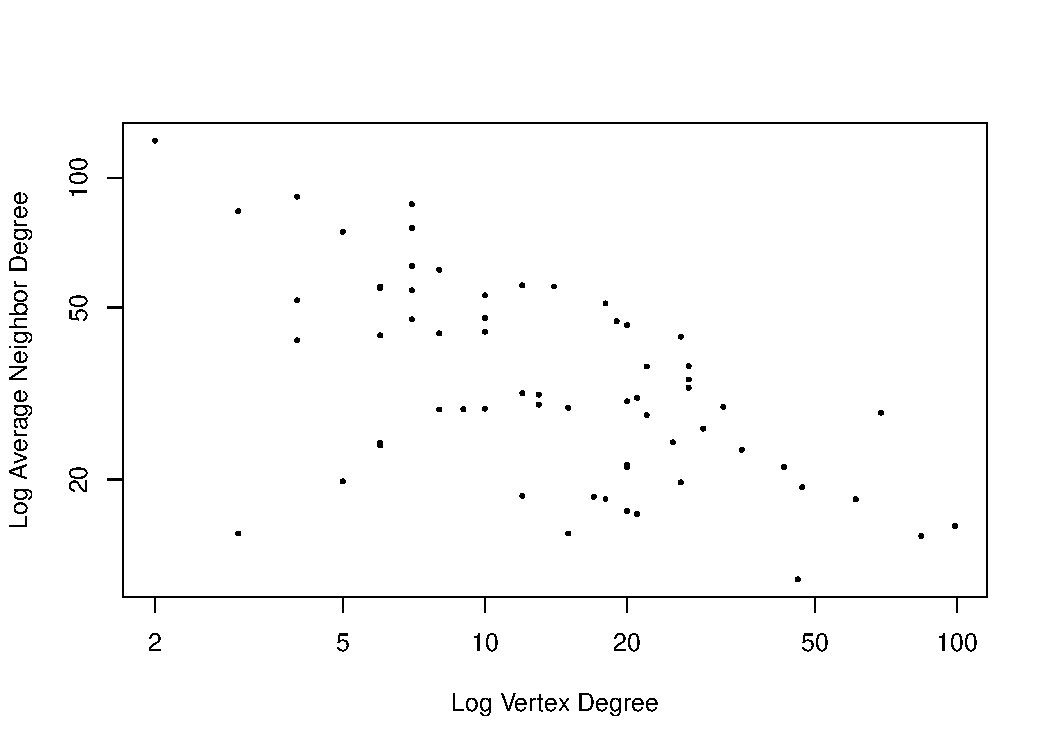
\includegraphics[scale=0.65]{Chapters/tb/logAvgDegree}
\caption{Log-Average Neighbor degree Distribution of the TB Co-authorship network}
\label{tb_fig2}
\end{figure}

After converting the multigraph network in a weighted graph, the network results in a simple graph of 173 vertices and 1,502 weighted edges. Closeness centrality ranges between $3.68\times 10^{-5}$ and $3.28\times 10^{-4}$ with a median of $3.18\times 10^{-4}$. Betweenness measures range between 0 and 3,077 with a median of 12.49. A network visualization with the vertices' size proportional to betweenness centrality measures clearly reveals the presence of broker authors (Figure \ref{tb_fig5} and Table \ref{table: tb_list}). The median Eigenvectors is 0.087 and a mean of 0.138. Eigenvectors measures reveal the presence of author hubs in the network suggesting the presence of closed collaboration groups. Table \ref{table: tb_list} presents a list of the 10 author hubs with the highest Eigenvectors values.\\
Edge betweenness centrality measures identify co-authorship collaboration ties that are important for the flow of information. Table \ref{table: tb_list} presents the top 10 most important collaboration ties for the flow of information in the TB Co-authorship network in Benin.\\

\begin{table}[h!]
\caption{List of the most important authors and collaborations in the Tuberculosis Co-authorship network}
\label{table: tb_list}
\centering \small
\begin{tabular}{l}
  \toprule
\textbf{Top 10 Brokers}\\
%\hline
\hspace{20pt}AFFOLABI DISSOU\\
\hspace{20pt}GNINAFON MARTIN\\
\hspace{20pt}DE JONG BOUKE C\\
\hspace{20pt}TREBUCQ ARNAUD\\
\hspace{20pt}ODOUN MATHIEU\\
\hspace{20pt}ANAGONOU SEVERIN\\
\hspace{20pt}WACHINOU PRUDENCE\\
\hspace{20pt}FAIHUN FRANK\\
\hspace{20pt}KASSA FERDINAND\\
\hspace{20pt}ADE SERGE\\
\hline
\textbf{Top 10 most connected authors (Top 10 network hubs)}\\
\hspace{20pt}GNINAFON MARTIN\\
\hspace{20pt}AFFOLABI DISSOU\\
\hspace{20pt}ANAGONOU SEVERIN\\
\hspace{20pt}MERLE CORINNE S C\\
\hspace{20pt}TREBUCQ ARNAUD\\
\hspace{20pt}OLLIARO PIERO L\\
\hspace{20pt}RUSTOMJEE ROXANA\\
\hspace{20pt}LO MAME BOCAR\\
\hspace{20pt}LIENHARDT CHRISTIAN\\
\hspace{20pt}HORTON JOHN\\
\hline
\textbf{Top 10 most important edges for information flow}\\
\hspace{20pt}ODOUN MATHIEU -- GNINAFON MARTIN\\
\hspace{20pt}FAIHUN FRANK -- DE JONG BOUKE C\\
\hspace{20pt}ODOUN MATHIEU -- TREBUCQ ARNAUD\\
\hspace{20pt}ZELLWEGER J P -- GNINAFON MARTIN\\
\hspace{20pt}TREBUCQ ARNAUD -- ADJONOU CHRISTINE\\
\hspace{20pt}ODOUN MATHIEU -- WACHINOU PRUDENCE\\
\hspace{20pt}AFFOLABI DISSOU -- BAHSOW OUMOU\\
\hspace{20pt}AFFOLABI DISSOU -- TOUNDOH N\\
\hspace{20pt}AFFOLABI DISSOU -- BEKOU W\\      
\hspace{20pt}AFFOLABI DISSOU -- MAKPENON A\\
\hline
\textbf{Weak articulation point}\\
\hspace{20pt}WACHINOU PRUDENCE\\
\bottomrule
\end{tabular}
\end{table}

\subsection{Network Cohesion}
Overall, 28 maximal cliques were detected in the network among which 1 clique of size 10, 2 cliques of size 5, and 2 cliques of size 4. The largest clique has size 10. \\The TB co-authorship network has a density of 0.10095 indicating that the baseline probability of collaboration tie formation is 10.095\%. The network also has a transitivity of 0.6305 meaning that 63.05\% of the connected triples in the network are close to form triangles. The transitivity metrics is a measure of the global clustering of the network.\\The network is not connected and a census of all the connected components within the network reveals the existence of a giant component that dominates all the other connected components. The giant component of the TB co-authorship network includes 90.8\% (157 vertices) of all the vertices in the network with the other components alone carrying less than 0.1\% of the vertices in the network (Fig. \ref{tb_fig5}). 

\begin{figure}[h!]
\centering
\hspace{1.5cm}
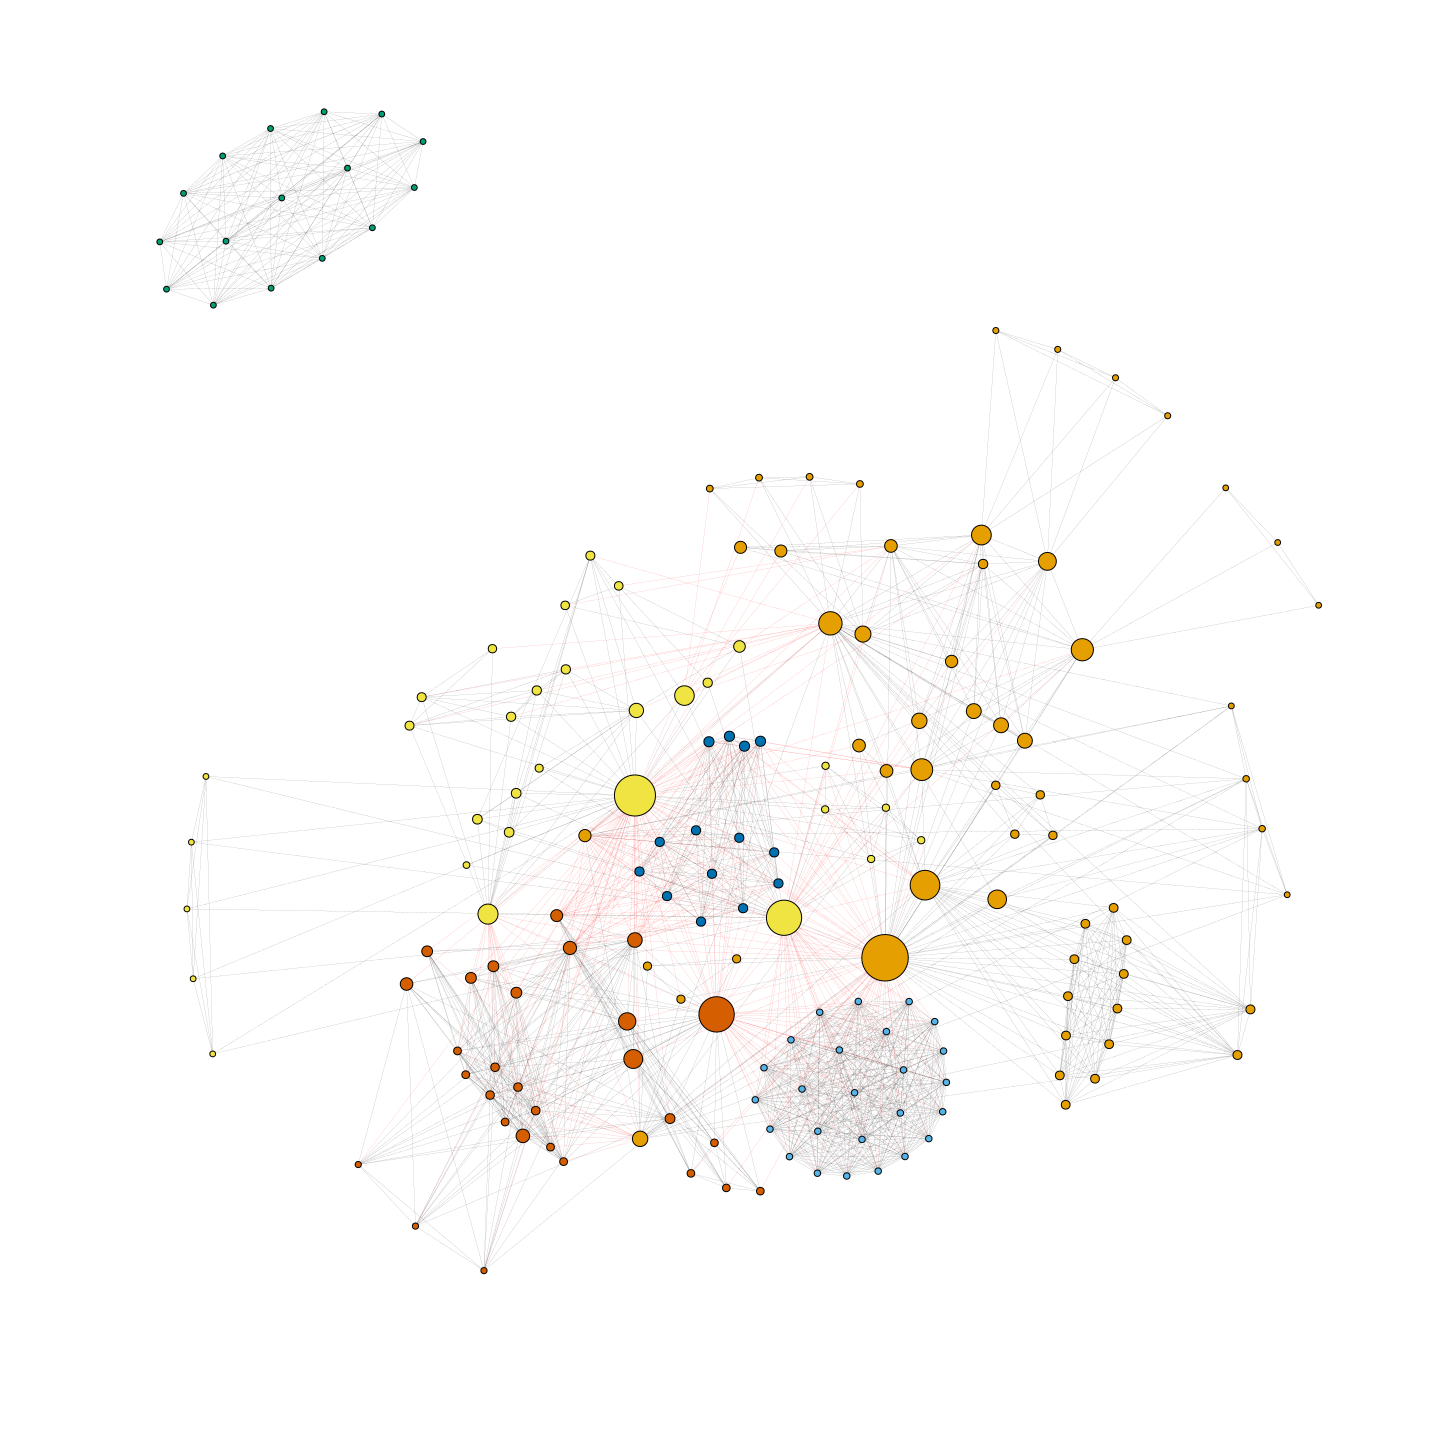
\includegraphics[scale=0.35]{Chapters/tb/tbnet}
\caption{Topological Structure of the Tuberculosis Co-authorship Network. Authors (vertices) of the same color belong to the same research community or cluster}
\label{tb_fig5}
\end{figure}

Information flow assessment of the network via cut vertices reveals the existence of a single author as the most vulnerable vertex in the network (Table \ref{table: tb_list}). The cut vertex constitute the weak articulation point of the TB co-authorship network. Cut vertices represent a measure of the vulnerability of the network \cite{kolaczyk_statistical_2014}.\\
The agglomerative hierarchical clustering method identifies 6 different research communities (or clusters) in the network. Sizes of the clusters range between 14 and 58 authors. Out of the 6 research clusters or communities detected, 5 are in the giant component. Figure \ref{tb_fig5} displays the giant component of the network with each different colors representing each of the 5 research communities. \\

\section{Modeling}
\subsection{Mathematical Modeling}
From the hierarchical clustering method of community detection, 6 different clusters/communities were detected in the co-authorship network out of which 5 form a giant component. One of the question of interest in this section is whether the number of communities detected is expected or not. To provide an answer to this question, we performed 1,000 Monte Carlo based simulations to test the significance of this observed characteristics of the TB co-authorship network. Figure \ref{tb_fig3} clearly demonstrates that the number of communities detected is unusual from the perspective of both Classical random graphs and generalized random graphs (p-value < 0.0001). From the Classical random graph model, the expected number of communities was 4.734 (95\%CI: 4.70 -- 4.77). Similarly, the expected number of communities from the generalized random graph model is 5.34 (95\%CI: 5.29 -- 5.38).

\begin{figure}[h!]
\centering
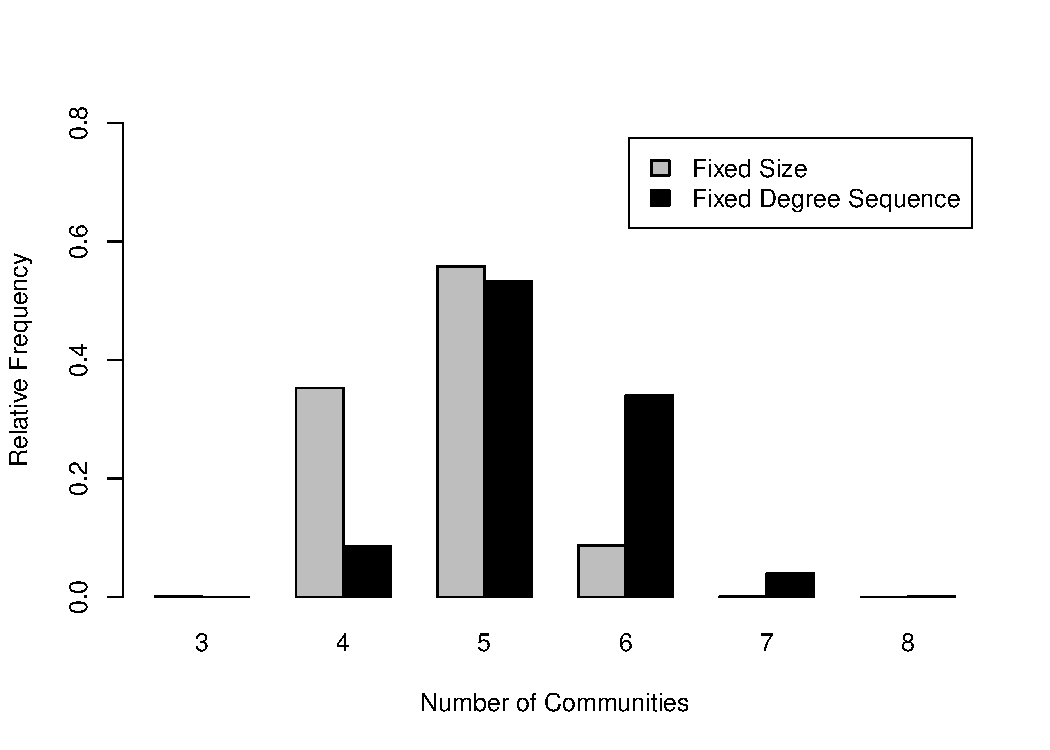
\includegraphics[scale=0.65]{Chapters/tb/randomComm}
\caption{Monte-Carlo simulations of the TB network: Number of detected communities by the random graph models}
\label{tb_fig3}
\end{figure}

Figure \ref{tb_fig4} displays the number of detected research communities using the Barab\'asi-Albert's preferential attachment and the Watts-Strogatz models. Here too, the observed number of communities was extreme per both models (p-value < 0.0001). The expected number from the Watts-Strogatz model simulations is 3.017 (95\%CI: 3.01 -- 3.03) and 13.77 (95\%CI: 13.70 -- 13.85) from the Barab\'asi-Albert model simulations. 

\begin{figure}[h!]
\centering
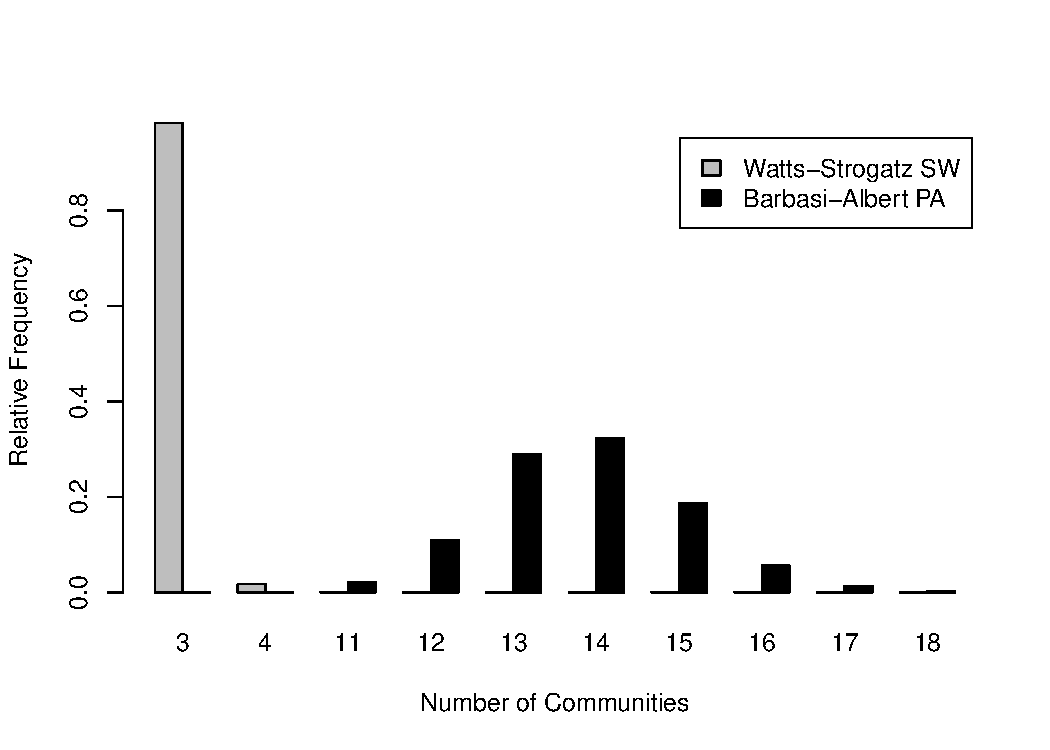
\includegraphics[scale=0.65]{Chapters/tb/mechanisticComm}
\caption{Monte-Carlo simulations of the TB network: Number of detected communities by the Watts-Strogatz and the Barab\'asi-Albert models}
\label{tb_fig4}
\end{figure}

We also compared the clustering coefficient and the average shortest-path length. Let's recall that the observed clustering coefficient is 0.614. One one hand, there was substantially more clustering in our TB co-authorship network than expected from both random graph models (p-value < 0.0001). The expected clustering coefficients was 0.10087 (95\%CI: 0.10068 -- 0.10107) and 0.1937 (95\%CI: 0.1934 -- 0.1939) respectively for the classic random graph and the generalized random graph models.\\
On the other hand, there was substantially less clustering in our TB co-authorship network than expected the Watts-Strogatz Small World model which expected clustering was 0.7259 (95\%CI: 0.7258 -- 0.7260).\\
We observed an average shortest-path length of 2.126 in the TB co-authorship network. This observed shortest-path length is significantly larger than what was expected from the random graph models (p-value < 0.0001) and significantly lower than what was expected from Watts-Strogatz small world model and the Barab\'asi-Albert preferential attachment model (p-value < 0.0001).\\The average shortest-path length was 2.0548 (95\%CI: 2.0546 -- 2.0550) and 2.072 (95\%CI: 2.0715 -- 2.0726) respectively for the classic random graph and the generalized random graph models.\\For the Watts-Strogatz small world and the Barab\'asi-Albert models, the average shortest-path length is respectively 2.623 (95\%CI: 2.616 -- 2.631) and 6.06 (95\%CI: 6.03 -- 6.09).\\~\\
We performed the same simulations on the giant component of the network with similar results leading to the same outcomes.

\subsection{Statistical Modeling}
%For the purposes of modeling the temporal dynamic of collaboration ties formation, we subset the network in different temporal snapshots. We subset the network, generating snapshots in a certain way that balanced the number of edges across the years. Such an uneven subsetting improved the robustness of our models and ensured model convergence. We ended up with 7 snapshots representing respectively the following timestamps: 1996 -- 2006, 2007 -- 2009, 2010 -- 2011, 2012 -- 2013, 2014, 2015 and 2016. %\\
%Figure \ref{fig:tb_dynNetwork} displays the topological structure of the snapshots of the different time steps.

\subsubsection{Stochastic Block Model}
\label{sec:tb_results_sbm}
The SBM identifies 14 classes with a degree of latitude of 9 to 14 classes being reasonable (See ICL plot on figure \ref{fig:tb_sbmgof}).

\begin{figure}[h!]
\centering
\hspace*{-1cm}
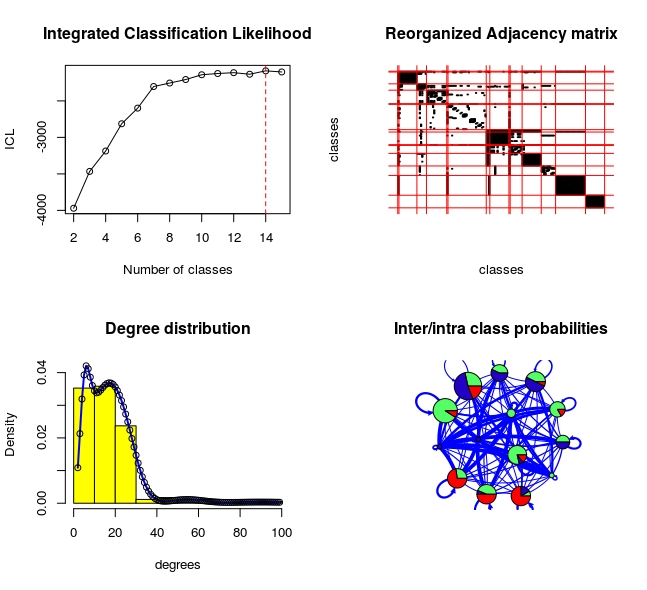
\includegraphics[scale=0.85]{Chapters/tb/statMod/tb_sbm}
\caption{Summary of the goodness-of-fit of the SBM analysis on the Tuberculosis co-authorship network.}
\label{fig:tb_sbmgof}
\end{figure}

The fitted SBM describes well the observed degree distribution. The vertices in the network depicting the inter/extra probabilities represent the 14 identified classes, with each one of them divided into a pie chart displaying the proportion of authors of international affiliations (lightgreen), authors of regional or other African affiliations (red), and authors affiliated to Beninese research institutions (blue). Generally, the dominance across the classes of international and regional players is observed. From the inter/intra probability network shows denser ties inter class ties. Looking at the pie charts, we can see that the classes are heterogeneous of almost all the classes with most of the classes having the same sizes (\ref{fig:tb_sbmgof}). Figure \ref{fig:tb_sbmdist} presents the distribution of the classes by affiliation types. \\

\begin{figure}[h!]
\centering
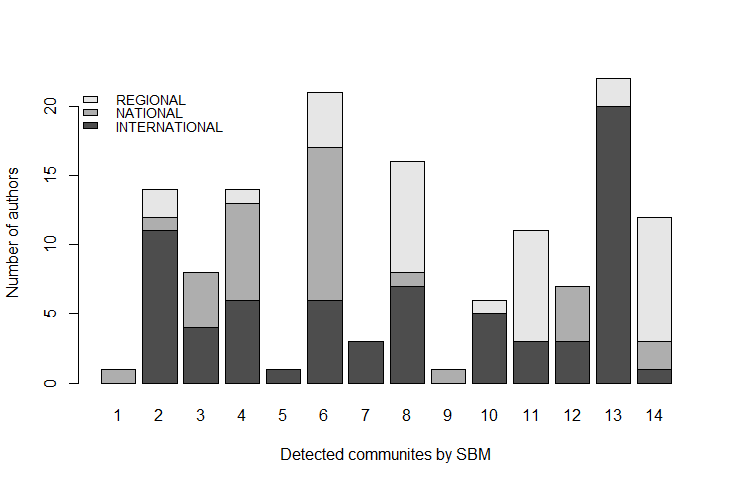
\includegraphics[scale=0.8]{Chapters/tb/statMod/tb_barplot2}
\caption{Distribution of national, international and regional authors by communities detected by the SBM in the TB network.}
\label{fig:tb_sbmdist}
\end{figure}

%On figure \ref{fig:hiv_sbmgof2}, we present the SBM results emphasizing the largest classes (with more than 20 members). Here, we can confirm that smaller classes tend to collaborate more among themselves and in-class collaborations tend to occur more.
%
%\begin{figure}[h!]
%\centering
%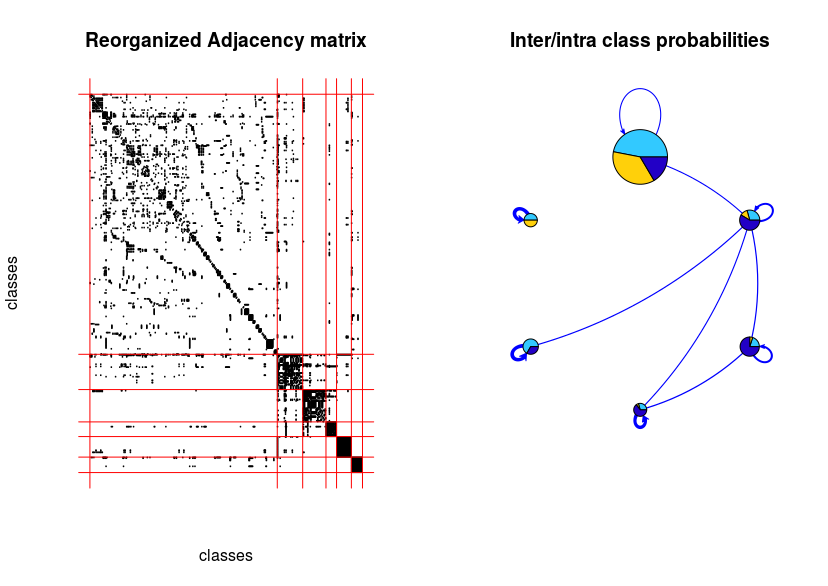
\includegraphics[scale=0.65]{Chapters/hiv/statMod/hiv_sbm2}
%\caption{Summary of the goodness-of-fit of the SBM analysis highlighting interactions between the largest classes of the HIV/AIDS co-authorship network.}
%\label{fig:hiv_sbmgof2}
%\end{figure}

\subsubsection{Exponential Random Graph Model}
\label{sec:tb_results_ergm}
We fit multiple ERGM method (Table \ref{tab:tb_ergm}). In the null model (model 1), the inverse logit of the coefficient associated with the intercept (edge term) is $0.10$ which is the baseline probability of collaboration ties establishment and also the density of the TB co-authorship network.

\begin{table}
\begin{center}
\hspace*{-1cm}
\small
\begin{tabular}{@{}lcclclcl@{}}
\toprule
           &  & Model 1 &  & Model 2  &  & Model 3\\ \cmidrule{3-3} \cmidrule{5-5} \cmidrule{7-7}            &  & Estimate ($SE$) &  & Estimate ($SE$)  &  & Estimate ($SE$) \\ \midrule
           Network structural predictor &  &   &  &  &  \\
\hspace{10pt}Intercept(edge) & & $-2.19 \; (0.03)^{***}$ & & $-7.84 \; (0.16)^{***}$ & & $-7.86 \; (0.17)^{***}$ \\ \\
Number of times cited        & &       --  & & $\hspace{6pt}0.01 \; (0.00)^{***}$ &  & $\hspace{6pt}0.01 \; (0.00)^{***}$  \\
Number of collaborations     & &  --  & & $\hspace{6pt}0.08 \; (0.00)^{***}$ &  & $\hspace{6pt}0.07 \; (0.00)^{***}$  \\
Number of publications       & &  --  & & $-0.05 \; (0.01)^{**~~}$ &  & $\hspace{6pt}0.01 \; (0.02)^{~~~~}$   \\
Homophily on cluster assignment &  &   --  &  & $\hspace{6pt}6.02 \; (0.13)^{***}$ &  & $\hspace{6pt}6.12 \; (0.14)^{***}$  \\
Homophily on collaboration type   &   & -- &   & $\hspace{6pt}0.83 \; (0.10)^{***}$ &  & $\hspace{6pt}0.90 \; (0.10)^{***}$  \\ \\
Factor attribute effect (collaboration type) &  &    &  &  &   &   \\
\hspace{10pt}International   &  & --   &  & --   &  & $REF$\\
\hspace{10pt}National        & &  --   &  &  -- & & $-0.40 \; (0.09)^{***}$ \\
\hspace{10pt}Regional        & &  --   &  & --  & & $\hspace{6pt}0.22 \; (0.08)^{**}$   \\
\midrule
AIC           &  & $\hspace{6pt}9737.42$  &  & $\hspace{6pt}3776.48$  &  & $\hspace{6pt}3747.34$ \\
BIC           &  & $\hspace{6pt}9745.03$  &  & $\hspace{6pt}3822.12$  &  & $\hspace{6pt}3808.20$ \\
Log Likelihood   &  & $-4867.71$        &  & $-1882.24$         &    & $-1865.67$ \\
\bottomrule
\multicolumn{4}{l}{\scriptsize{$^{***}p<0.001$, $^{**}p<0.01$, $^*p<0.05$}}
\end{tabular}
\caption{ERGM of the TB Co-authorship Network.}
\label{tab:tb_ergm}
\end{center}
\end{table}

Model 2 including all nodal variables, a homophily term on collaboration type and on cluster assignment improved tremendously compared to model 1 (See AIC, BIC and model likelihood in table \ref{tab:tb_ergm}). We note a decrease in the edge effect (Coefficient $=-7.84$, $p<0.001$) with the associated conditional probability (given all the other terms in the model) estimated at $0.039\%$. For the remaining terms in model 2, we observed a positive and significant effect except for the number of publications. Model 3 including the collaboration type as factor term, improved substantially compared to model 2. We therefore chose model 3 as our final model. One unit increases the number of citation, increases the odds of collaboration ties establishment by $1\%$. A one unit increase in the number of collaborations is associated with a $7.25\%$ increase in the odds of collaboration ties establishment. The coefficient associated with the number of publications is insignificant. Model 3 further proves that the process underlying the structure of the TB co-authorship network in Benin is mainly driven by homophily on cluster assignment or membership to a research community or group (Coefficient $=6.12$, $p<0.001$). The conditional probability of any two authors belonging to the same research group is estimated at $14.93\%$ compared to the baseline probability of $10\%$. The same probability changes to $30.15\%$ after adjustment by the collaboration type, and $32.08\%$ after adjusting for the number of citations, collaborations and publications. Compared to research affiliated to international institutions, researchers affiliated to Beninese institutions have $49.2\%$ average decrease in the odds of collaboration tie establishment. This average decrease is not statistically significant ($p>0.05$). For researchers affiliated to institutions other than Beninese institutions, the odds of collaboration tie establishment increases on average by $24.05\%$ compared to internationally affiliated researchers. Overall, model 3 estimated the probability of collaboration ties formation at $32.08\%$ for international researchers, $24.05\%$ for national researchers and $37.05\%$ for regional players. \\
Unfortunately, none of the models containing endogenous ERGM terms and/or the dyadic variables, attained convergence, we do not present those results in table \ref{tab:tb_ergm}.

\begin{figure}[!h]
\centering
\hspace*{-1cm}
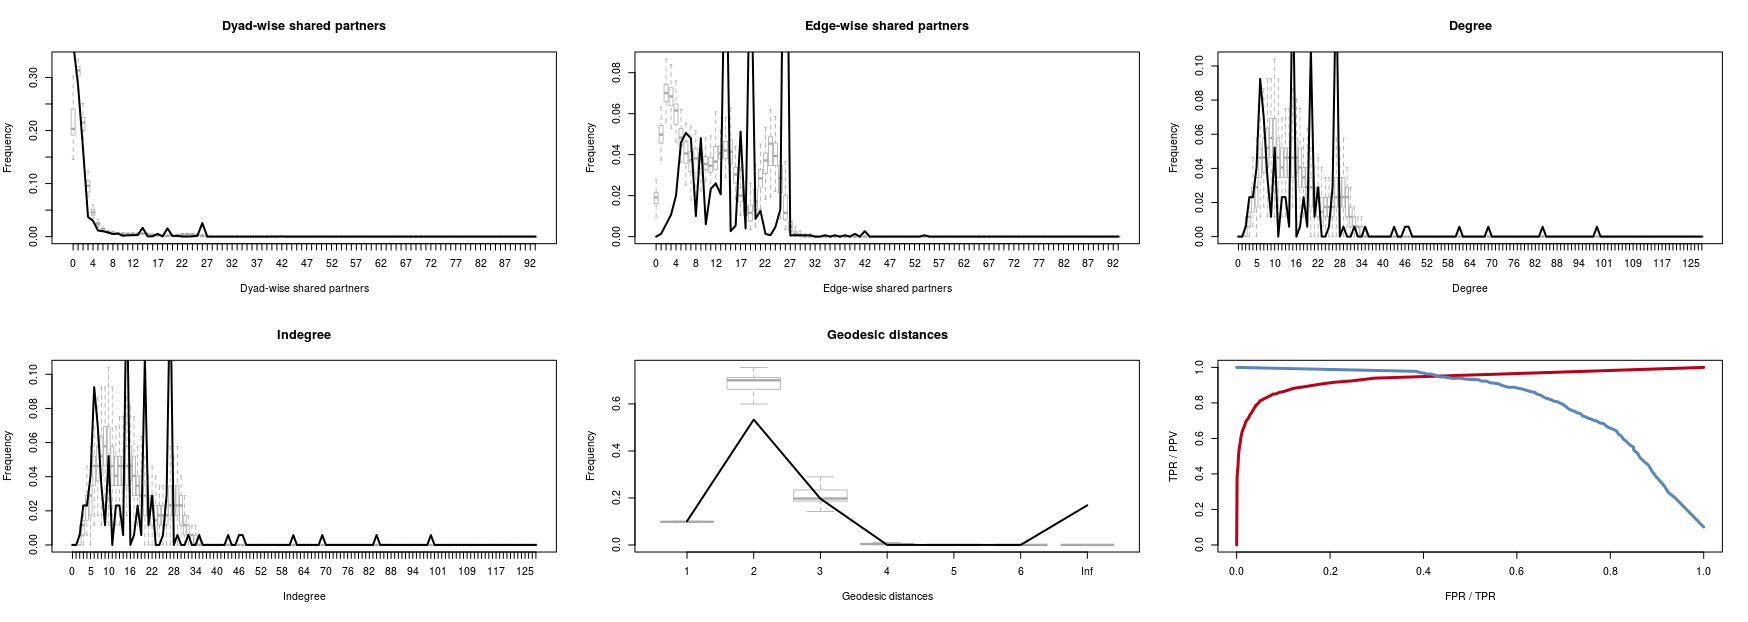
\includegraphics[scale=0.4]{Chapters/tb/statMod/tb_ergm_gof2}
\caption{ERGM goodness-of-fit of final model 3 assessment on the TB co-authorship network.%\\
%The observed properties are depicted by the black lines. Gray lines with circles represent the 95\% confidence intervals for the simulated network properties. Goodness-of-fit is asserted when the black lines lie in-between the confidence intervals lines.
}
\label{fig:tb_ergm-gof}
\end{figure}

Figure \ref{fig:tb_ergm-gof} presents the goodness-of-fit of the final model 3. It appears that the ERGM fits somewhat poorly the observed TB co-authorship network in terms of edge-wise, dyad-wise shared partners, degree, geodesic distances, triad census. Meanwhile, it displays a $93.7\%$ for the ROC model (in red) and $80.9\%$ for the Precision Recall (PR) model.

\subsubsection{Temporal Exponential Random Graph Model}
\label{sec:tb_results_tergm}
We subset the cumulative observed network in cinq snapshots according to the following time spans: 1996 -- 2008, 2009 -- 2011, 2012 -- 2013, 2014 -- 2015 and 2016. In figure \ref{fig:tb_dynNetwork}, we show the topological structure of the network snapshots for the different time steps.

\begin{figure}[!ht]
\hspace{-1.25cm}
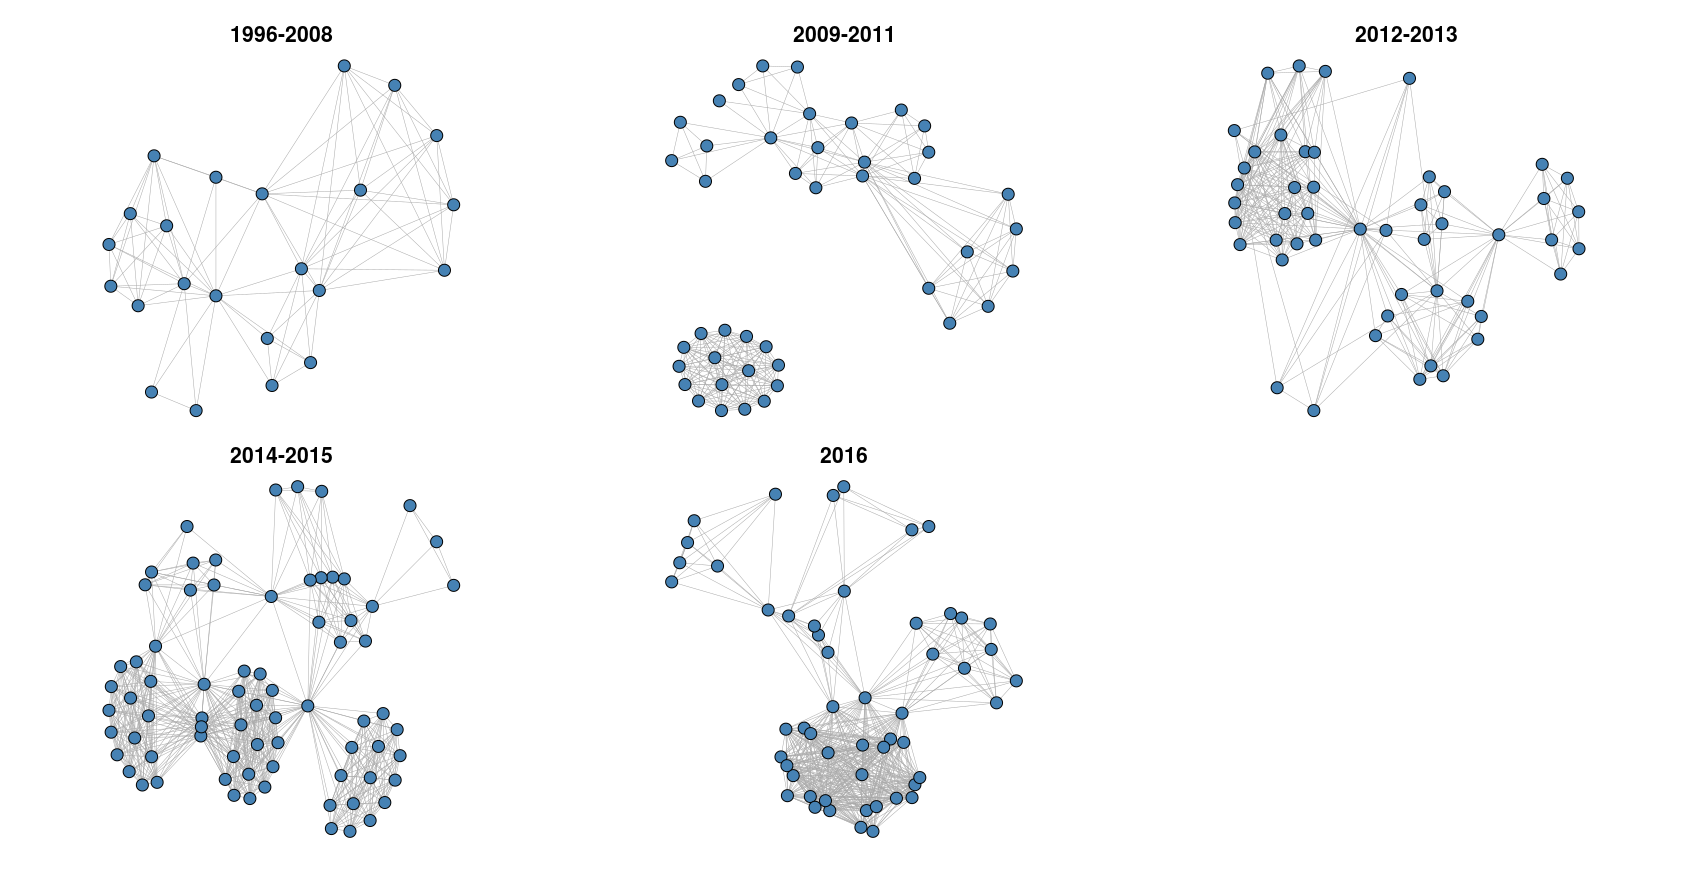
\includegraphics[scale=0.4]{Chapters/tb/statMod/tb_dynNetwork}
\caption{Topological structure of the different snapshots of the TB co-authorship network.}
\label{fig:tb_dynNetwork}
\end{figure}

Table \ref{tab:tb_tergm} summarizes the results of the different temporal models fit to the observed network. The coefficient for the edge term in the null pooled ERGM model 1 is estimated at $-3.75$ with an associated baseline pooled probability of collaboration tie formation of $2.30\%$, which is lower than the density of the observed cumulative TB network.\\
Model 2 adjusting for the nodal variables and the homophily terms improved slightly over the null model 1. Model 3 adjusted model 2 by including a factor attribute effect on the collaboration type with a slight improvement over model 2. Unlike the final model of the ERGM, we observed in model 3, a significant decrease of $23.4\%$ in the odds of researchers affiliated with Beninese institutions to collaborate compared to international researchers. This percentage decrease changes to $40.5\%$ after adjusting for the temporal dependencies in model 4. \\
We chose Model 4 as our final model because it significantly improved over model 3. The results of model 4 confirm our observation from the ERGM results that the process of collaboration tie establishment in the TB network is mainly driven by homophily on collaboration type and on membership to research groups or communities. \\
Temporal dependencies effects proved significant in the final model. A significantly positive dyadic stability effect accompanied with a significantly negative linear trends effect is observed. For dyadic stability, the coefficient is $0.44$ meaning that the odds of existent and non existent collaboration ties at one time point to remain the same at the next time point increased on average by $35.6\%$. In other words, the odds of new collaboration ties and non-ties to occur from one time point to another is $64.4\%$. Overall, the probability of international authors to establish a stable collaboration tie is $15.71\%$ versus $11.71\%$ and $16.11\%$ respectively for national and regional researchers.\\
The goodness-of-fit assessment of the final TERGM model 4 is presented in figure \ref{fig:tb_tergm-gof}. Regarding the endogenous network statistics, we observe a better fit of the final TERGM model 4 compared to the final ERGM model 3. In other words, the simulated network by model 4 show a good fit to the observed TB network data. The AUC of the ROC curve of model 4 is estimated at $83.2\%$ meaning that $83.2\%$ of the times, model 4 accurately predicting ties in the last snapshot. While this performance is lower than the performance of the final ERGM model 3 from the previous section, the walktrap and edge betweenness modularity distributions from model 4 predicted well the observed ones. Finally, the walktrap community comembership prediction displays an AUC of $71.4\%$.

\begin{table}
\begin{center}
\caption{Temporal ERGM of the TB Co-authorship Network.}
\label{tab:tb_tergm}
\hspace*{-1cm}
\scriptsize
\begin{tabular}{@{}lcclclclcl@{}}
        \toprule
           &  & Model 1 &  & Model 2  &  & Model 3 &  & Model 4\\ \cmidrule{3-3} \cmidrule{5-5} \cmidrule{7-7} \cmidrule{9-9}
           &  & Estimate ($SE$) &  & Estimate ($SE$)  &  & Estimate ($SE$) &  & Estimate ($SE$)\\
\midrule
Network structural predictor & & & & & & & & \\
\hspace{10pt}Intercept(edge)    &  & $-3.75 \; (0.02)^{***}$ & & $-10.07 \; (0.15)^{***}$ & & $-10.01 \; (0.16)^{***}$ & & $-8.62 \; (0.28)^{***}$ \\\\
Number of times cited       &  &       --    &  & $\hspace{6pt}0.00 \; (0.00)^{*~~~}$   &  & $\hspace{6pt}0.00 \; (0.00)^{~~~~}$      &  & $-0.00 \; (0.00)^{**~}$  \\
Number of collaborations    &  &         --  &  & $\hspace{6pt}0.14 \; (0.00)^{***}$ &  & $\hspace{6pt}0.14 \; (0.00)^{***}$ &  & $\hspace{6pt}0.16 \; (0.00)^{***}$  \\
Number of publications      &  &      --     &  & $\hspace{6pt}0.68 \; (0.03)^{***}$ &  & $\hspace{6pt}0.72 \; (0.03)^{***}$ &  & $\hspace{6pt}0.57 \; (0.03)^{***}$  \\
Homophily on cluster assignment   &  & --     &  & $\hspace{6pt}5.24 \; (0.11)^{***}$ &  & $\hspace{6pt}5.23 \; (0.11)^{***}$ &  & $\hspace{6pt}5.40 \; (0.13)^{***}$  \\
Homophily on collaboration type   &  &   --   &  & $\hspace{6pt}0.69 \; (0.08)^{***}$ &  & $\hspace{6pt}0.69 \; (0.08)^{***}$ &  & $\hspace{6pt}0.73 \; (0.09)^{***}$  \\\\
Factor attribute effect (collaboration type) & & & & & & & & \\
\hspace{10pt}International & & -- & & -- & & $REF$ & & $REF$ \\
\hspace{10pt}National  &  &  --   &  &   --   &  & $-0.21 \; (0.07)^{**~}$ &  & $-0.34 \; (0.08)^{***}$ \\
\hspace{10pt}Regional &  &    --  &  &   --   &  & $\hspace{6pt}0.03 \; (0.07)^{~~~~}$ &  & $\hspace{6pt}0.03 \; (0.08)^{~~~~}$    \\\\
Temporal dependencies & & & & & & & & \\
\hspace{10pt}Dyadic stability  &  &  --  &  &  -- &  &   --  &  & $\hspace{6pt}0.44 \; (0.07)^{***}$  \\
\hspace{10pt}Linear trends     &  &  --  &  &  -- &  &   --  &  & $-0.36 \; (0.06)^{***}$ \\
\midrule
AIC    & & $\hspace{6pt}431184.00$   & & $\hspace{6pt}419860.54$ & & $\hspace{6pt}419853.82$ & & $\hspace{6pt}253170.25$   \\
BIC    & & $\hspace{6pt}431205.66$ & & $\hspace{6pt}419936.36$ & & $\hspace{6pt}419951.30$ & & $\hspace{6pt}253284.48$    \\
Log Likelihood    & & $-215590.00$ & & $-209923.27$ & & $-209917.91$ & & $-126574.12$ \\
\bottomrule
\multicolumn{5}{l}{\scriptsize{$^{***}p<0.001$, $^{**}p<0.01$, $^*p<0.05$}}
\end{tabular}
\end{center}
\end{table}

\begin{figure}[!h]
\centering
\hspace*{-1cm}
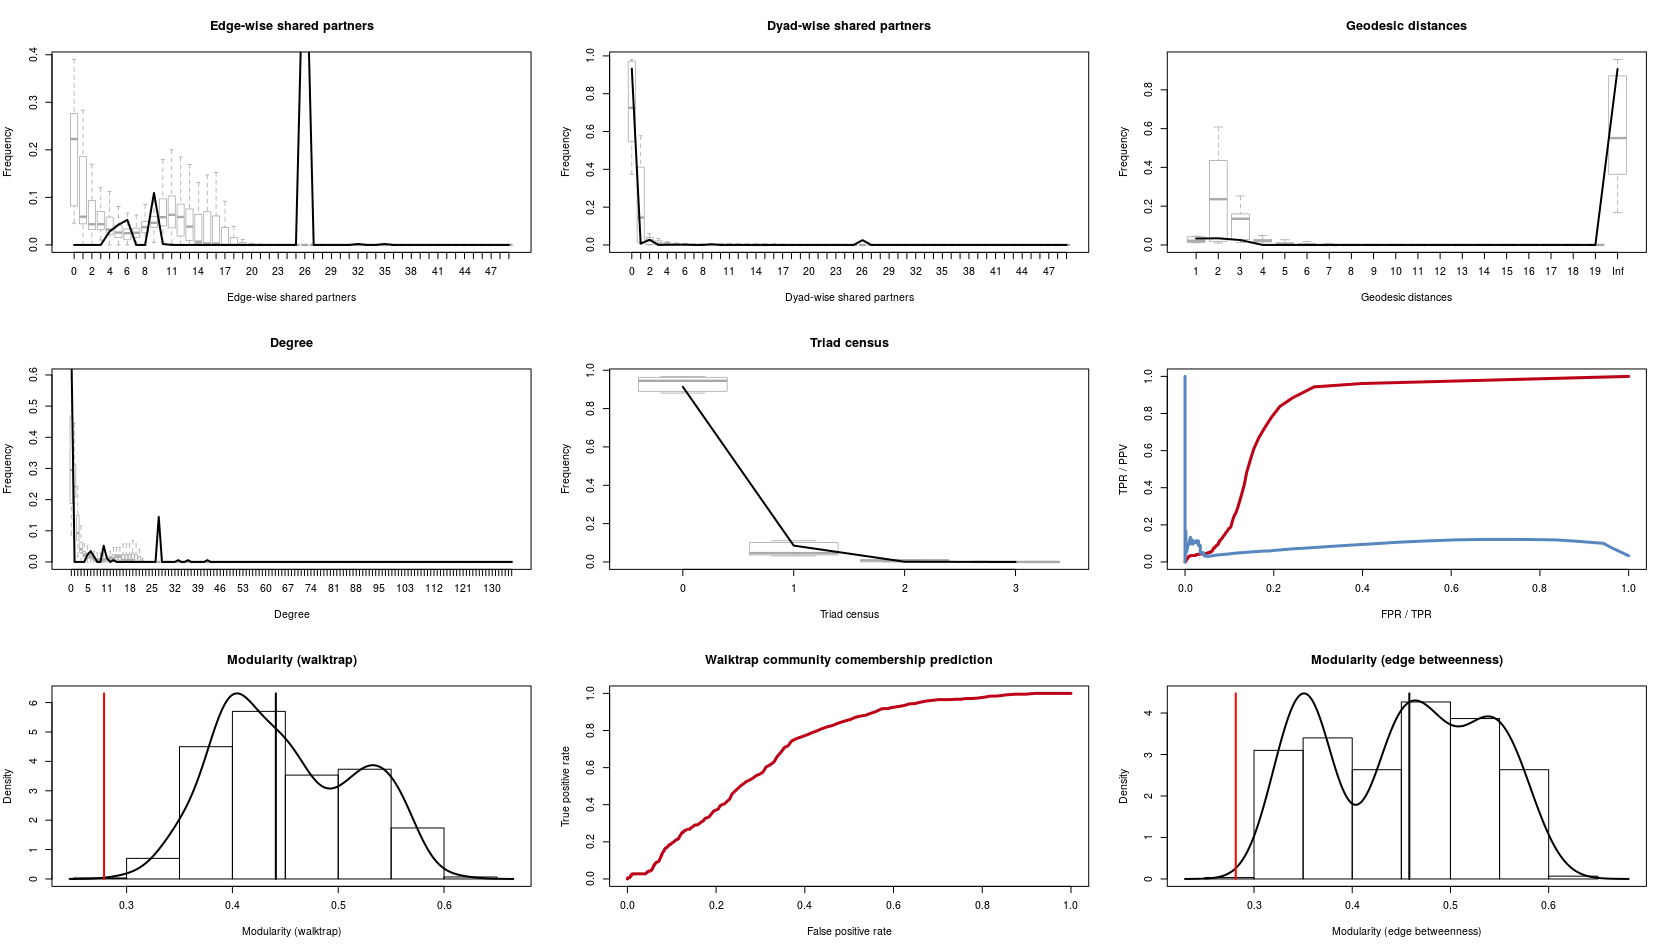
\includegraphics[scale=0.4]{Chapters/tb/statMod/tb_tergm_gof}
\caption{Goodness-of-fit assessment for the final TB TERGM Model 4 with temporal dependencies of the TB co-authorship network.}
\label{fig:tb_tergm-gof}
\end{figure}

\pagebreak
\subsubsection{Latent Network Model}
\label{tb_sec:results_lnm}
On the 3-dimensional visualization of the TB co-authorship network presented on figure \ref{fig:tb_lnm_viz}, the layouts are determined according to the inferred latent eigenvectors from the no pair-specific model (on top), the model containing nodal covariates (middle), and the model containing nodal and dyadic covariates (bottom). Blue vertices represent authors affiliated to Beninese research institutions, Red vertices are authors affiliated to international institutions, Gold vertices represent authors affiliated to African research institutions other than Benin, and White vertices represent authors with no determined affiliations. Node sizes are set to be proportional to the betweenness value of each vertex, with bigger nodes emphasizing key broker authors in the network. \\
The first visualization represents the null LNM model with no pair-specific covariates. It shows mainly three clusters. The largest cluster appears more spatially heteregeneous than the other two. It is also the largest cluster that contains the majority of the authors affiliated with Beninese research institutions. The other two clusters seem to be dominated respectively by international and regional researchers. This model displays fits reasonably well to the observed TB network ($AUC=0.912$).  This observation suggest a significant effect of geography in the odds of collaboration tie establishment. After adjusting for the nodal covariates (second visualization), there is less structure left to be captured by the latent variables and the clustering is no more apparent. Adding dyadic attributes to the model leads to similar outcome despite an increase in terms of performance ($AUC=0.974$). \\
On figure \ref{fig:tb_lnm_roc}, we present the ROC curves of each of the LNM models containing the nodal covariates and the null model.

\begin{figure}[!h]
\center
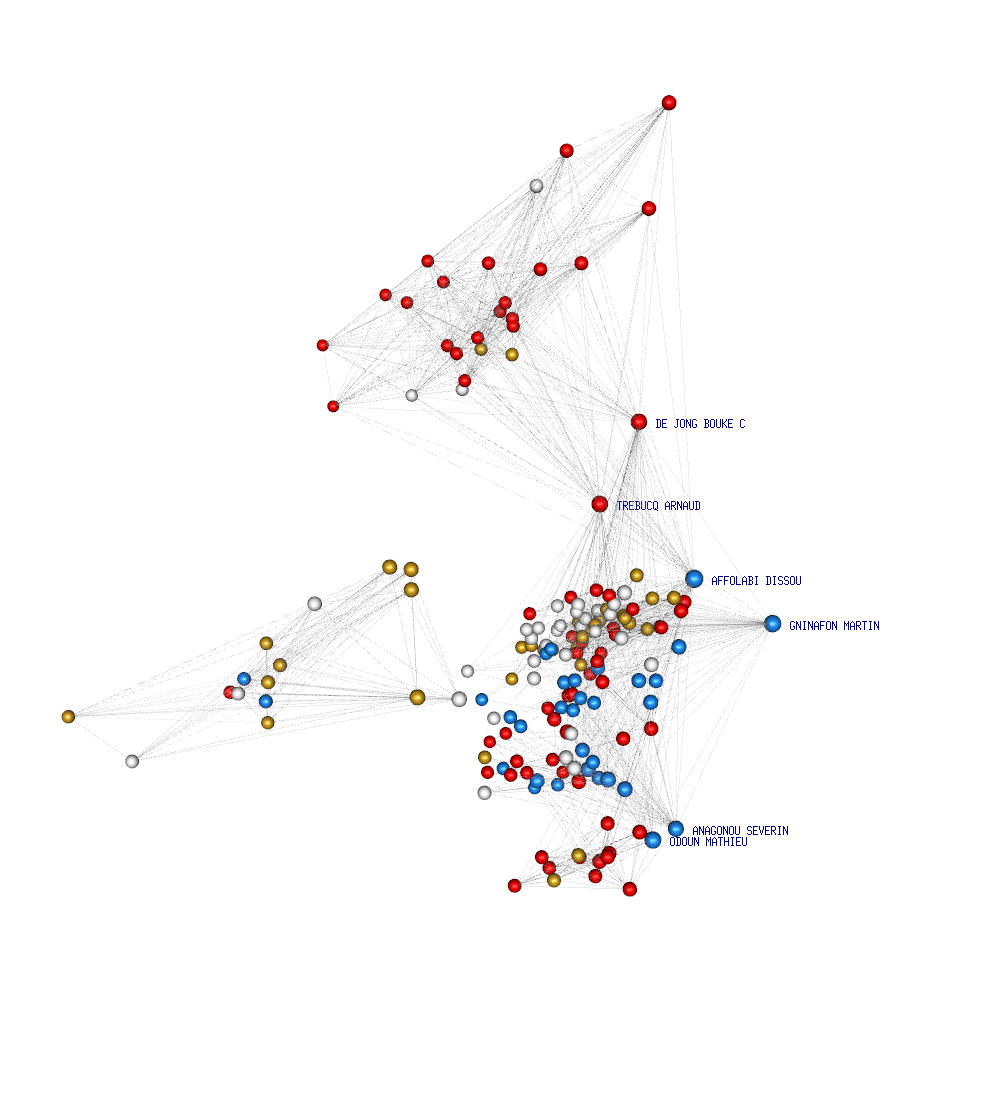
\includegraphics[scale=0.22,trim={5cm 2cm 2cm 0}]{Chapters/tb/statMod/lnm_mod1.png}
\vspace{0px}\\
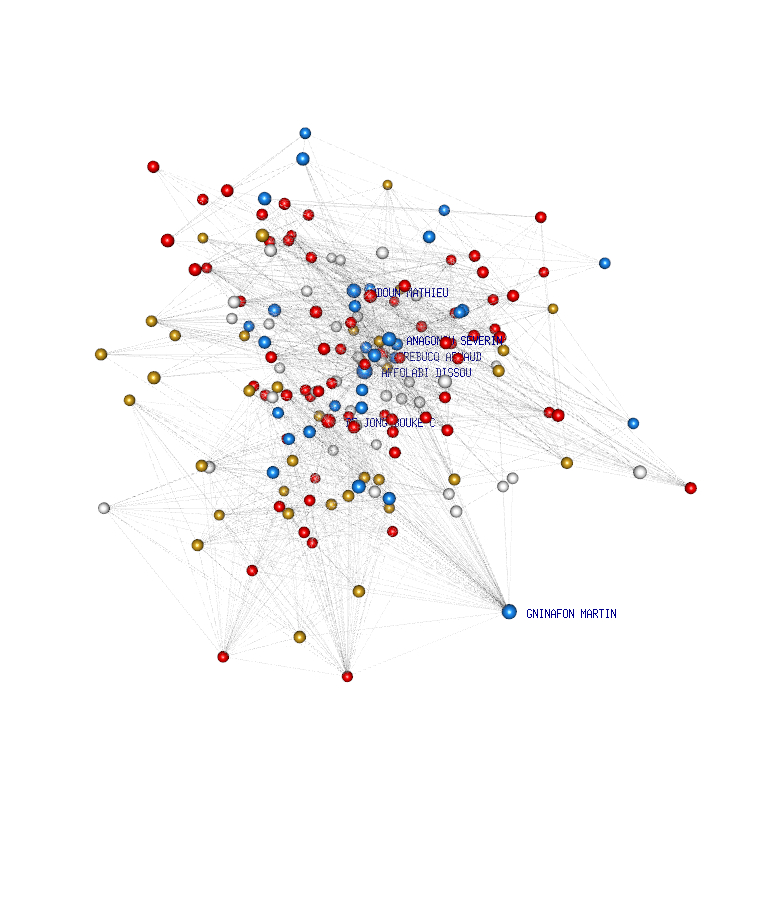
\includegraphics[scale=0.22,trim={5cm 2cm 2cm 5cm}]{Chapters/tb/statMod/lnm_mod5_AllNodal.png}
\vspace{2px}\\
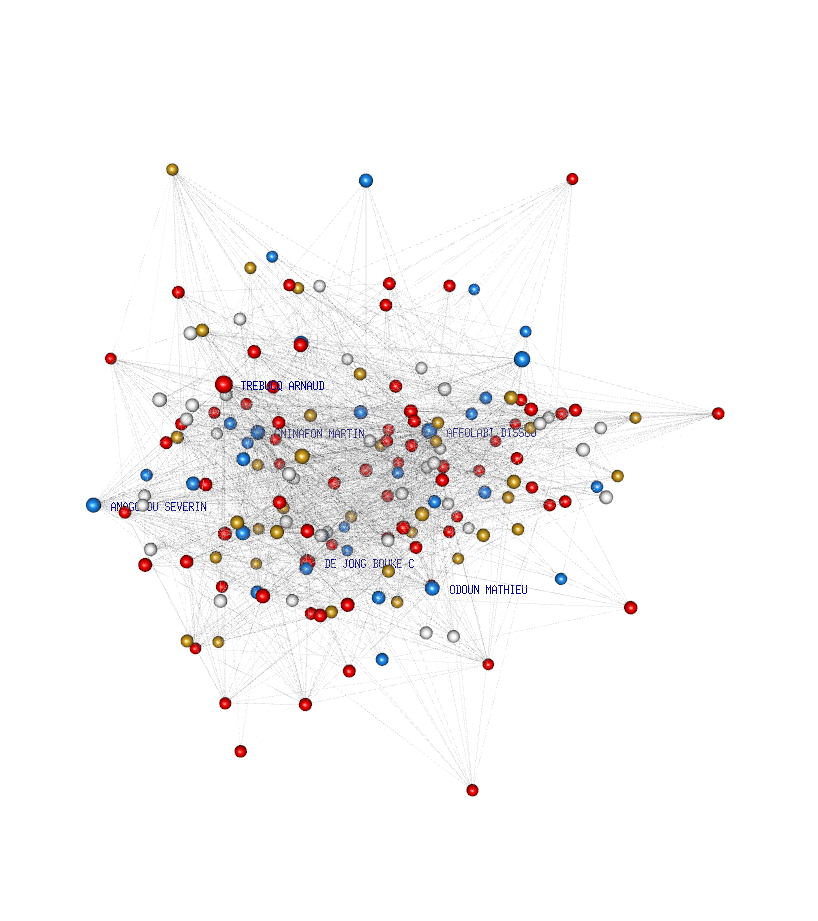
\includegraphics[scale=0.2,trim={5cm 5cm 5cm 5cm}]{Chapters/tb/statMod/lnm_mod7_All.png}
\caption{Visualizations of the TB co-authorship network with layouts determined according to the inferred latent eigenvectors in the LNM models.
% with no pair-specific covariates (top), nodal covariates (middle), and all covariates (bottom).
}
\label{fig:tb_lnm_viz}
\end{figure}

\begin{figure}[!h]
\centering
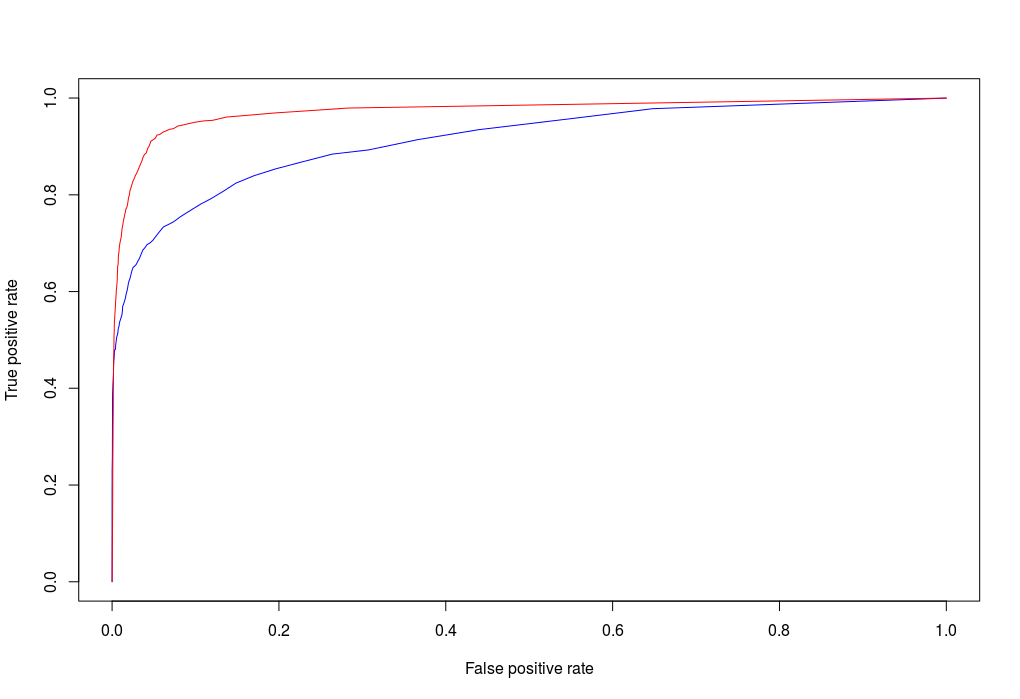
\includegraphics[scale=0.5]{Chapters/tb/statMod/tb_lnm_ROC.png}
\caption{ROC curves comparing the goodness-of fit of the TB co-authorship network for the model specifying (i) no pair specific covariates (blue) and the model specifying (ii) nodal covariates (red)%, and (iii) nodal and dyadic covariates (green), respectively
.}
\label{fig:tb_lnm_roc}
\end{figure}

\section{Discussion and Conclusion}
\label{sec:tb_discussion}
This chapter provides insights in the structural characteristics of the TB co-authorship network in Benin over the last 20 years. The evolution of the number of publications, authors and collaboration ties suggests a linear growth over the investigation period. We expected such findings given the place of TB in the public health concerns of Benin and the intensive effort towards the reduction of the incidence and the numerous campaigns of sensibilization \cite{world_health_organization_atlas_2016}. The findings from the descriptive analysis suggest that the mechanism underlying the formation of the TB co-authorship network in Benin is not random. However, we found inconclusive evidence of small world properties that further Monte-Carlo simulations disproved. The presence of closed research groups is supected given the non-trivial number of authors with higher order of magnitudes. The observed trend of prolific authors in the TB network to collaborate with less prolific ones is another indication suggesting that TB research is a low productivity research field in Benin. Only 37 published documents were found relevant to the present study. In fact, none of the top 10 key brokers in our TB co-authorship network, was in the list of the top most connected authors and therefore would suggest the relative absence of long publishing tenure authors in the network \cite{li_co-authorship_2013}. \\
The flow of information in the TB co-authorship network in Benin is slow as it only relies on a single author. A study by Salamatia and Soheili \cite{salamati_social_2016} on a co-authorship analysis of Iranian researchers in the field of violence reported similar but less extreme findings. For Bales et al. \cite{bales_social_2008,bales_evolution_2011}, the most important authors in co-authorship networks generally tend to be the ones with the highest degree of collaborations. For information flow, cut vertices provide a better approach to identifying vertices that are important to the long-term substainability of co-authorship networks \cite{kolaczyk_statistical_2014}. The only author identified as a cut vertex is therefore the most important author for information flow.\\
Our observed network has unexpected properties compared to classic small-world networks. Our TB co-authorship network displays properties that are more extreme than those of small-world and preferential attachement networks contradicting previous studies reporting co-authorship network as having small-world or preferential attachment properties \cite{gonzalez-alcaide_scientific_2012,wagner_network_2005}.\\
As the first advanced statistical model we applied to this network, the SBM identified heterogeneous classes with higher probabilities towards inter class ties establishment. This observation is different from what we observed for the malaria and the HIV/AIDS co-authorship network which both display low inter class probabilities and higher intra class probabilities of tie formation. \\
As in the malaria and the co-authorship network, the ERGM and TERGM results suggest that authors within the TB co-authorship network are more likely to establish collaboration ties within their research groups or communities. Although marginal, factors such as number of publications, number of citations and number of collaborations are associated to higher likelihood to establishing collaboration ties, confirming therefore our first hypothesis. Adding temporal dependencies to our ERGM models tremendously improved the fitness of the model to the observed network data, but at a cost of decreased performance compared to the model without temporal dependencies.\\
We expected the ERGM and TERGM models containing ERGM structural to converge for the TB co-authorship network given its relatively small size. Unfortunately, as for the malaria and the HIV/AIDS co-authorship networks, adding such terms to the the models proved computationally expensive. None of the models converged after $1,000$ iterations. We therefore, suspect the complexity of the network to have prevented the convergence of the models \cite{schmid_exponential_2017}. \\ 
With the LNM, we complement the ERGM and TERGM by adding an extra layer of analysis. Visualizing the effect of geography on the structure of the network, we notice that none of the nodal or dyadic covariates played a significant role in the spatial distribution of the network. Such an observation contradicts that of the malaria and the HIV/AIDS co-authorship network. The cluster demarcation observed with the null LNM model suggests that distance does play a significant role in collaboration tie formation in the TB co-authorship network. \\
As the co-infection TB-HIV/AIDS continues to be an important aspect of the public health strategies in the Republic of Benin, consolidating the knowledge generated from the many TB-related research is crucial. Furthermore, public health policies must empower and reinforce the different research groups or communities involved in the research effort. Our results suggest a need for a continuous support to the TB research network, considering its low productivity status in Benin. Such actions will help stabilize the research groups already involved in TB research and promote the junior scientists in the field. We finally believe that such measures will ultimately insure the long-term sustainability of the TB co-authorship and collaborative research network in Benin.

 % TB Co-authorship Network

%*******10********20********30********40********50********60********70********80

% For all chapters, use the newdefined chap{} instead of chapter{}
% This will make the text at the top-left of the page be the same as the chapter

\chap{AuthorVis: A Co-authorship Visualization and Scientific Collaboration Prediction tool}

\section{Background}
In this chapter, we propose a co-authorship network exploration, and link prediction tool specific to the three networks investigated in this dissertation. While many network visualization solutions have already been published, most of them are not specifically adapted to co-authorship network \cite{nakazono_nel_2006,odoni_visualisation_2017,liu_toolkits_2004,horak_forcoa.net:_2011}. 
% New citation to add: nakazono_nel_2006,odoni_visualisation_2017,liu_toolkits_2004,horak_forcoa.net:_2011,mena-chalco_brazilian_2014
Even those designed for visualizing co-authorship network have several limitations among others, their inability to satisfactorily display large networks, the lack of interactivity in the display, and the inability for the end user to control the display \cite{nakazono_nel_2006}.\\
Here, we present a tool that not only provides a visualization of each of the networks but allow the end user to query the network. Our integrates bibliometrics information to the visualization. With our proposed model, all the authorship information are embedded within the network, and at the fingertip of the end user. 
%We also provide a link prediction/recommendation tool to allow the users to predict future collaborations and recommend new ones. 
In the visualization interface, users can select a particular node or author to emphasize its subnetwork, hover over a node to display author's information or select an edge between two nodes/authors to display information related to materials co-authored by the two nodes defining that particular edge. 

\section{Related work}
Various authors have proposed diverse tools for the visualizations of co-authorship networks. One of such tools has been reported by Liu and colleagues \cite{liu_toolkits_2004} who proposed an author navigator application for visual examination of co-authorhip networks. In their conception of the toolkits, the authors combined a web based application tool for the interactive navigation of the network and a Java based backend swing application for the management of CGI requests. To support Brazilian researchers, Barbosa and colleagues proposed \textbf{VRRC}, a web based tool for the visualization and recommendation of co-authorship network \cite{barbosa_vrrc:_2012}. According to its developers, \textbf{VRRC} provides an interactive visualization, an overview of the collaborations over time, and recommendations to initiate new collaborations and reinforce existing ones. \textbf{VICI}, another co-authorship visualization tool was proposed by  Odoni and colleagues \cite{odoni_visualisation_2017}. \textbf{VICI} combined a Python based backend system for the extraction and management of the network data and a web based frontend using Flask \cite{grinberg_flask_2014} to display the network. The visualization of the network was finally rendered using the Javascript D3.js \cite{bostock_d3._2012} library. \textbf{NeL$^2$}, a general purpose tool for the visualization of networks as a layered network diagram was proposed by Nakazono, Misue, and Tanaka \cite{nakazono_nel_2006}. They applied their tool to the visualization of co-authorship networks to visualize transitions in the network over a period of time, as well as various co-authorship data. \\
Another framework, the WebRelievo system was proposed for the visualization of the evolutionary processes of Web pages \cite{toyoda_system_2005}. Other techniques were also proposed for the visualization of co-citation networks \cite{chen_visualizing_1999}, and for the visualization of the relationship of scientific literature \cite{erten_simultaneous_2005}. \\
Here, we propose \textbf{AuthorVis}, a co-authorship visualization and scientific collaboration tool for Malaria, TB and HIV/AIDS research in Benin. In addition to providing the same features as the aforementioned tools, with \textbf{AuthorVis}, we propose a different approach to co-authorship network visualization. Our approach integrates network structure and network data, hence requires no data management using traditional database framework. In addition, our visualization allows the end-user to navigate the network with an interactive navigation panel, but also integrate published materials within the visualization interface.

\section{Design and Architecture}
\textbf{AuthorVis} is built to a Shiny dashboard with an R based backend system that managed each co-authorship network data as an igraph object \cite{csardi_igraph_2006}. The backend system allows the end user to query the system through the Shinyboard. It is combined to a Javascript web based frontend that displays the network graph, and handle user interactions with the network.

\subsection{Data}
Currently, \textbf{AuthorVis} is designed specifically for the visualization of the Malaria, Tuberculosis and HIV/AIDS collaborative network in Benin. We refer the reader to section \ref{sec:data_collection} for details on the collection and treatment of the co-authorship data. On the server end, each network data is maintained as an igraph object. Each submitted user query is interpreted and incorporated in an igraph function to extract the network data. Another igraph object is generated as a result and converted into a JSON data using a specific Python script.

\subsection{Network Visualization}
The frontend network visualisation is built using the Javascript D3.js \cite{bostock_d3._2012}. We built in a navigation panel allowing the user to interact with the network and control physics of network \cite{newman_physics_2008}. We incorporated several Javascript functions to design an intuitive and user friendly visualization interface. A mouse hover over a vertex displays a tooltip of details on the author represented by the vertex while a double-click on a vertex highlights the subnetwork of the identified network. We made edges clickable. Once an edge is clicked, the list of published materials co-authored by the two vertices defining the clicked edge is displayed in a panel on the right hand side. All published materials listed can be traced back to their publication page on the web via their DOI or the WOS accession number with a single click.


\subsection{Web Framework}
The whole system is built into a Shiny dashboard thanks to the R package \textbf{Shinyboard} \cite{chang_shiny:_2017,chang_shinydashboard:_2015}. Using the dashboard, the user can choose to use the prediction tool menu, or query and visualize the network data. We also provide within the dashboard all our Shiny codes and a link to our Git directory containing all our source codes. \\
The prediction tool is model based and used the ERGM models to calculate a probability of collaboration between two authors. A micro-interpretation of the model is provided based on the user query  \cite{desmarais_micro-level_2012}. \\
When the user chooses the visualization menu, an interface allows him to submit his query to the system. The query is interpreted and processed on the server end and the user is automatically prompted to a new visualization page.

\section{Deployment}
The visualization front-end is maintained by an Python http-server. The system is packed in a Docker container to facilitate its use and installation. We also made it accessible online via https://www....

\section{Future Directions}
Currently, \textbf{AuthorVis} is specifically built for Malaria, TB and HIV/AIDS in Benin. Future development will extend the tool to other research domain. We also aim at adding a general purpose module to \textbf{AuthorVis} for the visualization of any user-input co-authorship network. This will also require the integration of a data pre-processing module to facilitate the disambiguation and deduplication of co-authorship information. Finally, we will also incorporate a layered structured network visualization \cite{nakazono_nel_2006} functionality to the visualization in order to display temporal changes in the evolution of the co-authorship network.


%\section{Conclusion}
%Text for this section goes here... % Link Prediction & Authorship Prediction Tool Development

%*******10********20********30********40********50********60********70********80

% For all chapters, use the newdefined chap{} instead of chapter{}
% This will make the text at the top-left of the page be the same as the chapter
\clearpage  % Start a new page
\lhead{\emph{General Conclusion}}  % left side page header to "List of Tables"
\chapter*{General Conclusion}
%\chap{General Conclusion}
\addcontentsline{toc}{chapter}{General Conclusion}
In this dissertation, we have documented and described the collaborative pattern in Malaria, HIV/AIDS and TB research in Benin. 
Since co-authorship networks are dynamic in nature, the application of temporal or dynamic modeling techniques is the major strength of our research. Other strengths include its application of not only descriptive methods but also robust network analysis methods such as inferential methods like Monte-Carlo simulations, unlike most studies on co-authorship analysis. Our data mining strategy involved a robust machine learning algorithm that helped address the crucial issue of the disambiguation of authors names and assign a unique identification to each of them. This technique maintained a good quality of the data collected throughout the pre-processing and analysis steps. To the best of our knowledge, our study is the first to describe the malaria research collaborations network via co-authorship network analysis in Benin. It is also the first to apply statistical network models to investigate co-authorship network in a specific research area in an African country.\\%~\\
Our first approach to modeling our network relied on the use of SBM. In addition of being a model based clustering method, the SBM identified important organizational and interactional patterns in the network. It is worth noting that many of the studies on co-authorship network analysis are descriptive in nature. This study is one of the rare co-authorship network analysis to model a co-authorship network using advanced statistical models. ERGM is the leading approach to modeling network \cite{schmid_exponential_2017}. The literature has reported application of this model in studying various social network such as the analysis of friendship and obesity \cite{valente_adolescent_2009,de_la_haye_obesity-related_2010}, the exploration of the association between hormone and social network structure \cite{kornienko_hormones_2014}. Similarly to friendship networks, the use of ERGM to model co-authorship networks is easily justified. However, the size of our network prevented the fitting of complex models including dyadic and structural terms. In addition, our best model failed to adequately fit the observed network data. This lack of goodness-of fit, according to Hunter, Goudreau and Handcock \cite{hunter_goodness_2008}, could be improved by including the geometrically weighted edgewise shared partner, geometrically weighted dyadic shared partner, and geometrically weighted degree network statistics to our model. Although, we follow such recommendations by including these structural network statistics to our final model, the ERGM model failed to converge after a maximum of 1,000 iterations. Furthermore, at about 750 iterations, we notice that the processing became both computationally intensive and expensive in terms of CPU time and memory usage.  In a recently published paper, Schmid and Desmarais \cite{schmid_exponential_2017} acknowledged the difficulty of fitting network which size is of the order 1,000 vertices using ERGM. They recommended that using the maximum pseudolikelihood estimation (MPLE) instead of the Monte Carlo maximum likelihood (MCMLE) could tremendously reduce computation time. Having followed these recommendations too, the model containing dyadic and structural terms still failed to converge. Let's recall that our weighted co-authorship network contains 1,792 vertices for 95,707 edges. We suspect that the number of edges, the large size of the network added to the possibility of hidden/latent variables might justify the failure of the final model containing the dyadic and structural terms to converge. We remedy this situation by applying LNM to the observed network data. \\
The fact that we collected data only from the Web Of Science can be considered as an important limitation of this study. However, according to Falagas and colleagues \cite{falagas_comparison_2007}, who compared PubMed, Scopus, Web Of Science and Google Scholar in their paper, the Web Of Science appears as a reasonable scientific database source for our analysis. In addition, it proved to cover a wide range of both old and recently published papers. Falagas and colleagues \cite{falagas_comparison_2007} found PubMed to be the optimal choice in terms of scientific database. For that reason we did run the same bibliographic search in PubMed. Unfortunately, the Web Of Science returns more relevant data than PubMed. Another limitation worth noting is that this study only looks at a snapshot of the malaria research network on a static fashion. There is also a need to apply dynamic statistical models such as Temporal Exponential Random Graph \cite{leifeld_temporal_2015} and Dynamic Stochastic Block \cite{matias_statistical_2016} modeling to better understand the temporal dynamic of collaboration formation in this network. Yet another limitation is inherent to the nature of all co-authorship studies. Collaborators, in a co-authorship network, do not often come from the same scientific discipline, or do not play the same roles on a particular research project. The data we collected did not allow us to accurately assess or even infer the disciplines each author came from or their specific contribution in the published document.
 % Conclusion



%% Appendices -----------------------------------------------------
%\addtocontents{toc}{\vspace{2em}} % Add a gap in the Contents, for aesthetics
%\lhead{\emph{Appendices}}  % Change the left side page header to "Appendices"
%\appendix % Cue to tell LaTeX that the following 'chapters' are Appendices

%\clearpage
\pagestyle{plain} % The page style headers have been "empty" all this time,
\hypertarget{app:draft}{} 
\chapter*{\centering Appendix}
\addcontentsline{toc}{chapter}{Appendix}
\centering \textbf{Combined MEG and fMRI Exponential Random Graph Modeling for inferring functional Brain Connectivity.}
%\chap{Appendix: Neuroscience Manuscript Draft}
\pagebreak
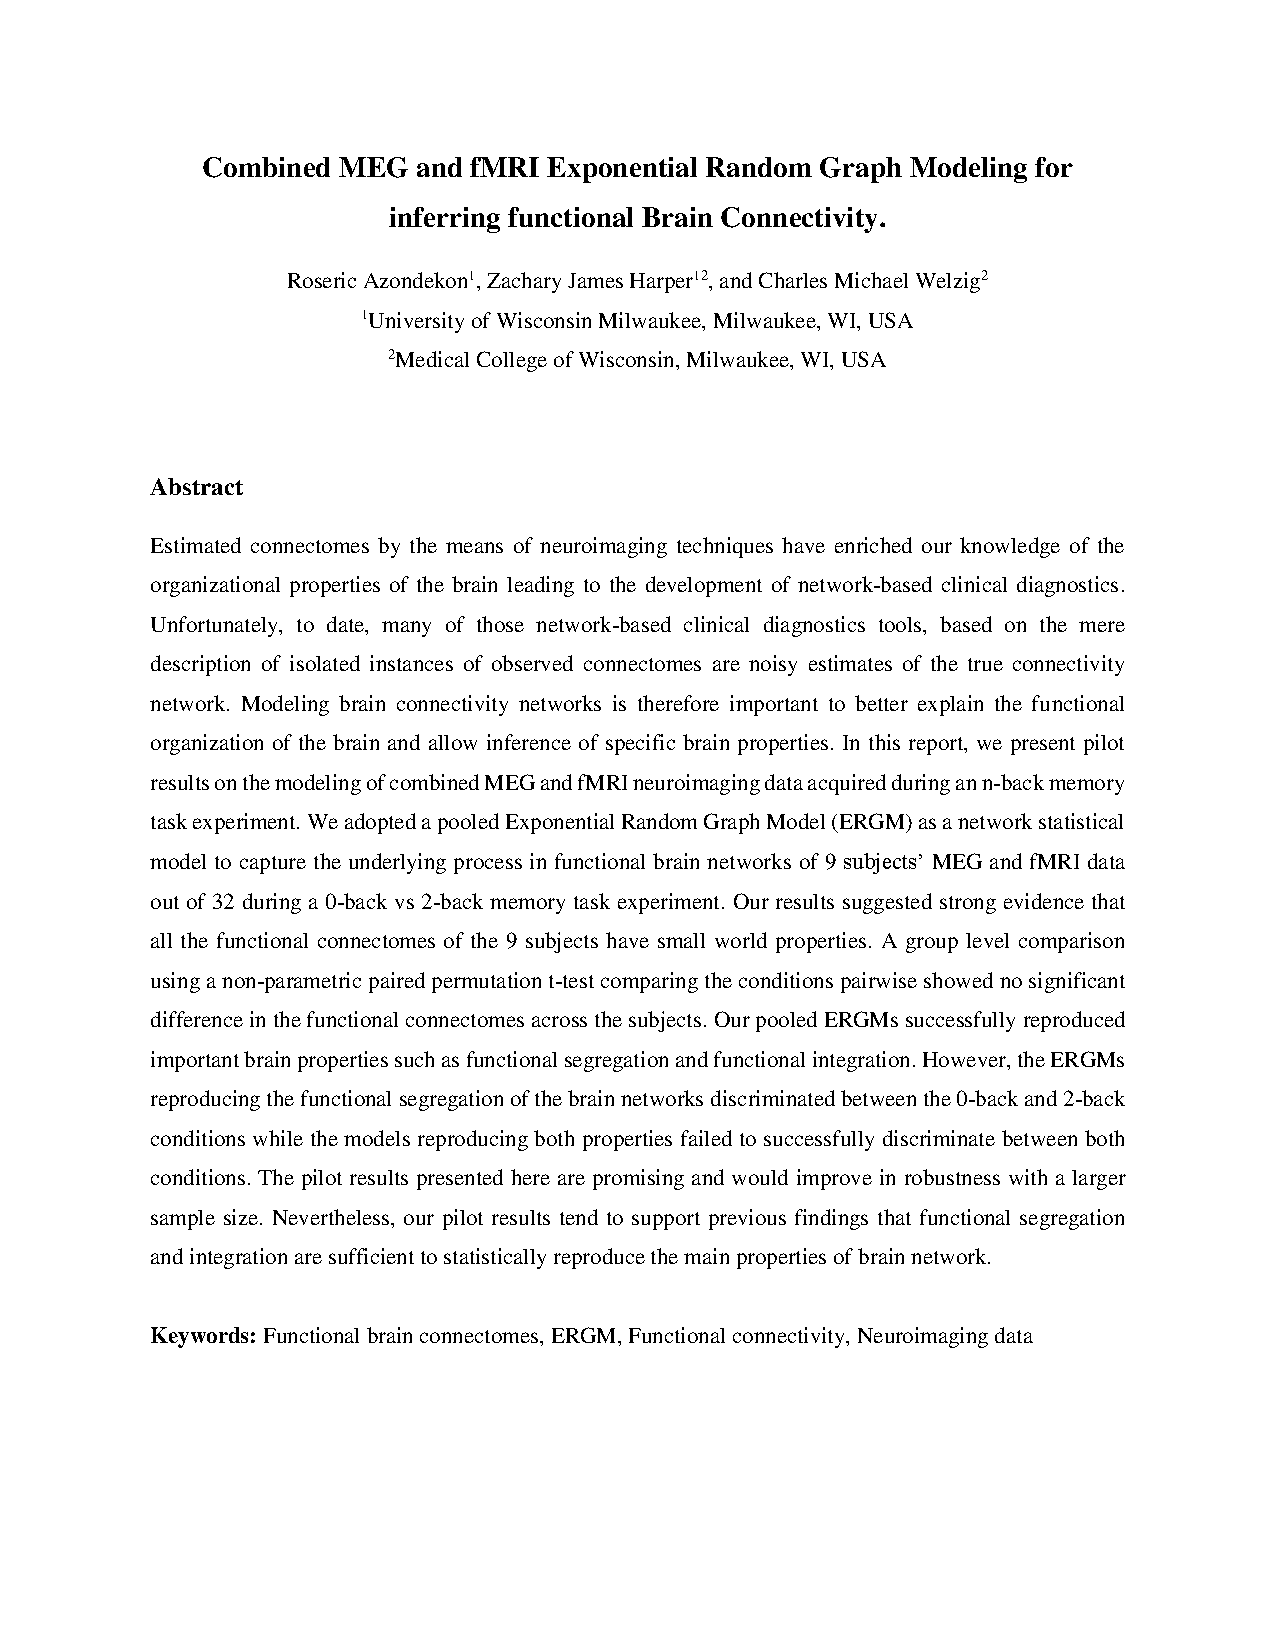
\includepdf[pages=-,offset=75 -75,pagecommand={}]{Files/ergm_brainNetwork.pdf} % Appendix Title

%\input{Appendices/AppendixB} % Appendix Title

%\input{Appendices/AppendixC} % Appendix Title


%% Bibliography ---------------------------------------------------
\backmatter % Cue to tell LaTeX that the following 'chapters' are Bibliography
\label{Bibliography}
\lhead{\emph{Bibliography}}  % left side page header to "Bibliography"
\bibliographystyle{unsrtnat}  % Use the "unsrtnat" BibTeX style for formatting the Bibliography
%\bibliographystyle{bmc-mathphys}
\begingroup
    \raggedright
    \sloppy
%\addbibresource{bibliography.bib}
    \bibliography{bibliography}  % The references (bibliography) information are stored in the file named "Bibliography.bib"
\endgroup 


\end{document}  % The End
%% ----------------------------------------------------------------